\documentclass[a4paper,12pt]{book}
\usepackage[a4paper, portrait, margin=0.5in]{geometry}
\usepackage[utf8]{inputenc}
\usepackage{graphicx}
\usepackage{braket}
\usepackage{dsfont}
\usepackage{amsmath}
\usepackage{mathtools}
\usepackage{cancel}
\usepackage{bbold}
\usepackage{titlepic}
\usepackage{hyperref}
\setcounter{secnumdepth}{3}
\setcounter{tocdepth}{3}

\newcommand{\numberset}{\mathbb}
\newcommand{\N}{\numberset{N}}
\newcommand{\R}{\numberset{R}}
\newcommand{\Z}{\numberset{Z}}


\begin{document}



\author{Giorgio Cambiè, Alessandro Marcelli}
\title{Appunti di Meccanica Quantistica}
\date{2019}

\titlepic{
\includegraphics[]{images/copertina.png}}


\frontmatter
\maketitle
\tableofcontents
 
\mainmatter


\chapter{Crisi della fisica classica}

\section{Corpo Nero}
	Idealmente un corpo nero rappresenta un oggetto che assorbe tutta l'energia della radiazione elettromagnetica incidente. \newline
In pratica potremo pensare ad esso come una cavit\`a (ad esempio sferica) su cui si trova un piccolo foro. se nel foro entra radiazione, questa verr\`a riflessa all'infinito al suo interno fino ad essere assorbita dalle pareti.

Trattando il problema classicamente, otteniamo che il potere emissivo della cavità sar\`a funzione di due fattori:

\begin{enumerate}
	\item la temperatura del sistema T
	\item la lunghezza d'onda della radiazione iniettata $\lambda $
\end{enumerate}	

ossia, in formule

\begin{equation}
\rho( \lambda, T) \sim \sigma T^4 \sim \frac{8\pi K_b T}{\lambda^4}
\end{equation}

Ma c'\`e un problema! Siccome in molti casi  $\lambda \to 0$, come per gli UV \newline ($10^{-8}$ m) e per i raggi $\gamma$ ($10^{-12}$ m),si avrebbe che 

\begin{equation}
\rho( \lambda, T)|_{T= cost.} \to \infty
\end{equation}

ossia avremmo la cosiddetta \textbf{catastrofe ultravioletta}.\newline
Questo ovviamente non succede, altrimenti il sole, essendo una fonte di UV, ci avrebbe gi\`a disintegrato da tempo.\newline
\newline
\newline
\noindent A questo punto entra in gioco \textbf{Planck}, chiedendosi: "sar\`a vero che la luce \`e un'onda? E se invece avesse una netta natura corpuscolare? E se la sua energia fosse discreta (o \textbf{quantizzata})?"

Il giovane genio Plack ipotizz\`o pertanto che la densit\`a di energia irradiata da un corpo nero fosse in realt\`a multiplo di un'energia quantizzata, ottenendo

\begin{equation}
\rho(\lambda. T) \sim \frac{8\pi h c}{\lambda^5} \frac{1}{e^{\frac{hc}{\lambda k T}} -1}
\end{equation}

Notiamo che espandendo in serie di Taylor questa converge.\\




\section{Effetto fotoelettrico}

Si nota quando, irradiando un metallo con onde elettromagnetiche, questo emette elettroni (un esempio pratico sono le scintille emesse durante la saldatura).

Venne scoperto da Hertz, il quale notò diversi fatti interessanti:

\begin{enumerate}

\item Il numero di elettroni emessi e la loro energia \textbf{non dipendono dall'intensit\`a della radiazione} (ossia dal numero di fotoni incidenti), ma \textbf{solamente dalla loro lunghezza d'onda $\lambda$.}

\item La quantità di corrente dipende invece dall'intensit\`a
\end{enumerate}

Tuttavia poteva ancora essere vera l'ipotesi ondulatoria della radiazione elettromagnetica, dato che \textbf{il fotone incide con una certa frequenza, viene assorbito da un'elettrone che oscilla come un dipolo e ne emette a sua volta uno con la stessa frequenza}. In realtà no.



\section{Effetto Compton}

Si tratta di scattering elastico dei fotoni incidenti sugli elettroni negli orbitali. Questo fenomeno cozza drammaticamente con la definizione ondulatoria della luce, dato che l'urto elastico è proprietà delle particelle. \newline
Compton scoprì che i fotoni scatterati avevano una diversa lunghezza d'onda rispetto a prima dell'urto, dipendente dall'angolo di impatto:

\begin{equation}
\Delta \lambda = \frac{h}{m_e c}(1 - cos(\theta))
\end{equation}

Elaboriamo meglio. Partiamo da due ipotesi:

\begin{enumerate}
	\item Il fotone viene solo assorbito
	\item L'angolo a cui viene emesso un fotone dopo l'assorbimento dipende solo da $\lambda$
\end{enumerate}

Quello che ci aspettiamo \`e di ritrovare su una lastra rivelatrice tutti i fotoni che faremo incidere sul bersaglio in un unico punto individuato da $\theta$.\newline
Sperimentalmente invece trovo che \textbf{il numero è diviso in $\theta$ e $\theta'$}. Allora se $\lambda \sim \theta$ avremo che $\lambda' \ne \lambda$. Questo però implica che tali fotoni sono stati deflessi e non assorbiti! 

 \begin{figure}[!htb]
	\center{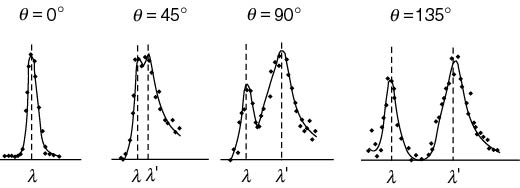
\includegraphics[width=\textwidth]
		{./images/4Idky.jpg}
	\caption{\label{fig:my-label} I = I($\lambda$)}}
\end{figure}

\section{Atomo di Bohr}

Lavorando sotto Rutherford, Bhor applicò l'ipotesi di Planck al suo modello atomico, enunciando tre postulati:

\begin{enumerate}
	
	\item Gli elettroni orbitano intorno al nucleo con orbite stabili (dette \textbf{stazionarie}) senza irraggiare. Possono muoversi da una all'altra ma non stare in mezzo.
	
	\item Le orbite stazionarie si trovano a distanze dal nucleo tali che il momento angolare orbitale degli elettroni sarà multiplo della costante di Plack ridotta.
	
	\begin{equation}
	|p_e|= m_e v r= n \hbar
	\end{equation}
	
	\item Gli elettroni possono spostarsi da un'orbita all'altra solo se ricevono o cedono un valore soglia di energia, detto \textbf{quanto}, pari a 
	
	\begin{equation}
	\Delta E = E_2 - E_1 = h \nu
	\end{equation}

\end{enumerate} 

\section{Figure d'Interferenza per fasci di elettroni}

Il fenomeno dell'interferenza si nota classicamente solo in caso di meccanica ondulatoria.
Per\`o se onsideriamo invece ora un fascio di elettroni con energia 

\begin{equation}
E= pc = \frac{hc}{\lambda}
\end{equation}

E lo facciamo incidere su una superficie con due fessure poste a distanza 

\begin{equation}
\vec{\lambda}= \frac{h}{\vec{p}}
\end{equation}

Se dietro tale superfice poniamo una lastra di materiale sensibile, noteremo la tipica figura d'interferenza... ma com'è possibile se l'elettrone è una particella?

Quanto detto fino ad ora ci porta a due conclusioni:

\begin{enumerate}
	\item La radiazione elettromagnetica e gli elettroni hanno una doppia natura, sia ondulatoria che corpuscolare
	\item L'energia di questi oggetti è quantizzata, ovvero che ciascuno di essi ha un'energia discreta e contribuisce a livello globale, ossia
	
	\begin{equation}
	E_{tot}= \sum{E_i} = h\sum{\nu_i}
\end{equation}

\end{enumerate}

Sappiamo, grazie alle nozioni di ottica, che l'intensità di un fascio di fotoni è data da

	\begin{equation}
	I = (E_1 + E_2)^2 = E_1^2 + E_2^2 + 2E_1E_2
\end{equation}

Questo significa, nel caso di singola particella che deve passare o da una fessura o dall'altra, che \textbf{il fotone interferisce con se stesso}. Gli elettroni si comportano allo stesso modo!

Dunque, se in \textbf{ottica classica} avevamo

\begin{equation}
\rho (r,t)= \rho_1 (r,t) + \rho_2 (r,t)
\end{equation}

In \textbf{meccanica quantistica} ci troveremo con

\begin{equation}
\psi (x,t)= \psi_1 (x,t) + \psi_2 (x,t)
\end{equation}

\begin{equation}
\psi_i (x,t)= A_i cos(kx-\omega t)
\end{equation}


 \begin{figure}[!htb]
	\begin{center}{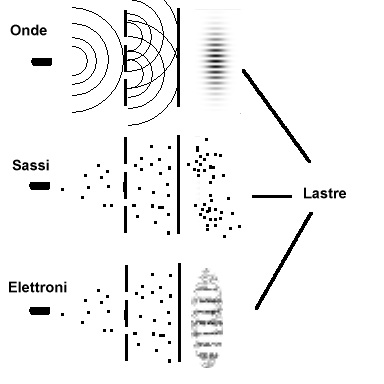
\includegraphics[width=.5\textwidth]
		{./images/Elettroni_e_fenditure.jpg}
		\caption{\label{fig:my-label} Rappresentazione del problema}}
	\end{center}
\end{figure}

\chapter{Introduzione alla meccanica quantistica}

\section{Notazione di Dirac e rappresentazione delle coordinate}
Diamo rapidamente la definizione delle grandezze che andremo a studiare. Il loro significato verrà spiegato nelle pagine successive.
\subsection{Notazione di Dirac}
\begin{enumerate}
	\item Ket, o vettore colonna 
		\begin{align}
			\ket{\psi} &= \left(
			\begin{array}{ccc}\psi_1 \\ \dots \\ \psi_n\end{array}
			\right)
		\end{align}
	\item Bra, o vettore riga
		\begin{align}
			\bra{\psi} &= (\psi_1^* \dots \psi_n^*)
		\end{align}
	\item Operatore
		\begin{align}
			\mathbf{\hat O} &= \left(
			\begin{array}{ccc}o_{11} & \dots & o_{1n} \\ \dots & \dots & \dots \\ o_{n1} & \dots & o_{nn}\end{array}
			\right)
		\end{align}
	\item Braket, o prodotto scalare
		\begin{align}
			\braket{\phi | \psi} &= 
			\left(\phi_i^* \dots \phi_n^* \right) \left(
			\begin{array}{ccc}\psi_1 \\ \dots \\ \psi_n\end{array}
			\right)
		\end{align}
	\item Modulo quadro di un vettore
	\begin{align}
		|\psi|^2 &=\braket{\psi | \psi} = 
		\left(\psi_i^* \dots \psi_n^* \right) \left(
		\begin{array}{ccc}\psi_1 \\ \dots \\ \psi_n\end{array}
		\right)
	\end{align}
\end{enumerate}

 \subsection{Rappresentazione di Schrödinger (o delle coordinate)}
 
 \begin{enumerate}
 	\item Funzione d'onda
 		 \begin{align}
 			\braket{x | \psi} &\rightarrow \psi(x,t) \in L_2
 		\end{align}
 	\item Operatore posizone applicato alla funzione d'onda
 		 \begin{align}
			q_i\ket{\psi} &\rightarrow x_i\psi(x,t)
 		\end{align}
 	\item Operatore impulso applicato alla funzione d'onda
		 \begin{align}
			p_i\ket{\psi} &\rightarrow -i\hbar \frac{\partial}{\partial x_i}  \psi(x,t)
		\end{align} 	
 	\item Prodotto scalare in rappresentazione di Schrödinger
 		 \begin{align}
	 			\braket{\phi | \psi} &\rightarrow \int \limits_{R^n} dx \: \phi^*(x,t)\psi(x,t) 
 		\end{align}
 	\item Modulo quadro in rappresentazione di Schrödinger
 		 \begin{align}
 			\braket{\psi | \psi} &\rightarrow |\psi(x,t)|^2 = \int \limits_{R^n} dx \: \psi^*(x,t)\psi(x,t)
 		\end{align}
 \end{enumerate}
 
\section{I postulati della meccanica quantistica}

Per semplicità, affronteremo il discorso dei postulati in 1D. 

\subsection{Principio di sovrapposizione}
	Ogni stato fisico può essere descritto in due modi:
	
	\begin{enumerate}
		
		\item tramite un \textbf{raggio di vettori} in uno spazio vettoriale complesso $H$ 
		
		(un raggio di vettori è composto da vettori proporzionali tra di loro con un fattore complesso).
		
		\item tramite una funzione di probabilità chiamata \textbf{funzone d'onda} $\psi(x,t) \in L_2$, definita come
	
	\begin{equation}
	\psi(x,t)= |\psi(x,t)|e^{i\theta}
	\end{equation}
	
	Per un sistema a più corpi avremo
		
	\begin{equation}
	\psi(x,t)= \prod_{n} \psi_n(x,t)
	\end{equation}
	\end{enumerate}

La probabilità di trovare una particella in un intervallo $[x_0, x_1]$ sarà data da 	

	\begin{equation}
	P(x \in [x_0, x_1])= \int_{x_0}^{x_1} dx \: |\psi(x,t)|^2
	\end{equation}

 Se la $\psi(x,t)$ esprime tutti i possibili stati di una particella, allora avremo che se 
	
	\begin{equation}
	\ket{\psi}= \sum_{n}c_n \ket{\psi_n} \rightarrow \psi(x,t)= \int dx \: c_n \psi_n(x,t)
	\end{equation}
	
avremo che
	
	\begin{equation}
	P(x)= \sum_{n} |c_n|^2= 1 
	\end{equation}
		
\subsection{Le osservabili}

In meccanica quantistica il concetto di misura di un'osservabile viene affrontato matematicamente come applicazione di operatori (che rappresentano le \textbf{osservabili}) su vettori (che rappresentano gli \textbf{stati del sistema}). 

Gli operatori associati alle osservabili sono Hermitiani, ossia 

\begin{equation}
\mathbf{\hat O} = \mathbf{\hat O^\dagger} \longleftrightarrow o_{ij}=o^*_{ji}
\end{equation}

e quindi $\exists$ una base di autovettori ortonormali in cui $\mathbf{\hat O}$ è diagonale con autovalori \textbf{o} $\in R$.\newline

Effettuare una misura \textbf{perturba il sistema}, facendolo \textbf{collassare}

\begin{equation}
\mathbf{\hat O} \ket{\psi}=\ket{\psi'}
\end{equation}

Se lo stato su cui stiamo effettuando la misura è autovettore dell'operatore in questione, avremo che

\begin{equation}
\mathbf{\hat O} \ket{\psi}=o\ket{\psi}
\end{equation}

Operativamente quindi la misura di un'osservabile può essere espressa come

\begin{enumerate}
	\item Notazione di Dirac: 
	\begin{equation}
\bra{\psi}	\mathbf{\hat O} \ket{\psi}=\bra{\psi} o \ket{\psi}= o \braket{\psi | \psi}= o \in R
	\end{equation}
	\item Rappresentazione di Schrödinger:
	
	\begin{equation}
\mathbf{\hat O} \ket{\psi} \rightarrow O(x)\psi(x,t)
	\end{equation}
	
	\begin{equation}
\bra{\psi}	\mathbf{\hat O} \ket{\psi}= \int_{-\infty}^{+\infty}dx \: \psi^*(x,t)O(x)\psi(x,t)
\end{equation}
	
\end{enumerate}


Presi due operatori $\mathbf{\hat A}$ e $\mathbf{\hat B}$, se questi sono Hermitiani avremo che 

	\begin{equation}
\mathbf{\hat A}\mathbf{\hat A^\dagger}= \mathds{1} =\mathbf{\hat B}\mathbf{\hat B^\dagger}
\end{equation}

e quindi 

\begin{equation}
[\mathbf{\hat A},\mathbf{\hat B}]= \mathbf{\hat A}\mathbf{\hat B} - \mathbf{\hat B}\mathbf{\hat A}=0 
\end{equation}


Allora si dice che i due operatori \textbf{commutano}, e che le osservabili che rappresentano sono \textbf{compatibili}, ossia che la misura di una sullo stato non disturba la misura dell'altra. 
In formule questo si rispecchia nel seguente modo

\begin{equation}
\left\{\begin{array}{ccc}

\mathbf{\hat A} \ket{\psi}= a\ket{\psi} \\ \mathbf{\hat B} \ket{\psi}= b\ket{\psi} \end{array}\right. \rightarrow \mathbf{\hat A}\mathbf{\hat B}\ket{\psi}=\mathbf{\hat B}\mathbf{\hat A}\ket{\psi}=ab\ket{\psi}
\end{equation}

in quanto

\begin{equation}
\mathbf{\hat A}\mathbf{\hat B}\ket{\psi}= \mathbf{\hat A}(\mathbf{\hat B}\ket{\psi})=\mathbf{\hat A}b\ket{\psi}=b\mathbf{\hat A}\ket{\psi}= ab\ket{\psi}
\end{equation}
 e viceversa. 
 
 Questo significa inoltre che $\exists$ una base di autovettori (detti \textbf{simultanei}) che diagonalizza entrambi.

\subsection{Probabilità di transizione} 

Data un'osservabile $\xi$, sappiamo che una sua misura sullo stato $\ket{A}$ causerà una transizione, con probabilità $P_i$. Definiamo quindi la \textbf{probabilità di transizione tre due stati} come

\begin{align}
P(\ket{A} \rightarrow \ket{B})= \frac{|\braket{B|A}|^2}{\braket{A|A}\braket{B|B}}
\end{align}

che è una definizione valida dato che

\begin{enumerate}
	\item non dipende dai singoli vettori ma dallo stato, in quanto eventuali fasi si eliminano.
	\item ha valori compresi fra 0 (stati ortogonali) e 1 max grazie alla \textbf{disuguaglianza di Schwartz}.
\end{enumerate}

\section{Conseguenze dei postulati}
 
\subsection{Osservabili non degeneri}
 
Data un'osservabile non degenere $\xi$ con spettro $\xi_i$, i suoi autovalori normalizzati a 1 $\ket{\xi_i}$ formano un sistema ortonormale completo.

\bigskip

L'ortogonalità è dovuta dal fatto che una misura su autostato non darà mai un altro valore, e la probabilità di transizione è quindi nulla:

\begin{align}
{}&P(\xi_i \rightarrow \xi_j)= |\braket{\xi_i|\xi_j}|^2 \\
&\braket{\xi_i|\xi_j} = \delta_{ij}= \left\{
\begin{array}{cc}
0 \quad i \neq j \\
1 \quad i = j
\end{array}
\right.
\end{align}


\bigskip

La completezza la dimostriamo per assurdo.

Supponiamo esista un vettore $\ket{A} \; t.c. \braket{A|\xi_i}=0 \; \forall i$, avremmo che

 $P_i= |\braket{A|\xi_i}|^2=0 \rightarrow P= \sum_i P_i=0$, il che  è impossibile.

\bigskip

Ogni vettore $\ket{A}$ può essere quindi scritto come

\begin{align}
\ket{A}= \sum_{i=1}^{+\infty} a_i \ket{\xi_i}
\end{align}

Possiamo anche notare che 

\begin{align}
\braket{A|A}= \sum_{i,j} a_i^* a_j \braket{\xi_i|\xi_j} = \sum_{i,j} a_i^* a_j \delta_{ij} = \sum_{i} |a_i|^2
\end{align}

Da cui ricaviamo due conseguenze:

\begin{enumerate}
	\item Affinché $\ket{A}$ sia autovettore di $H$ dovremo avere $\sum_{i} |a_i|^2<+\infty$
	\item Se $\ket{A}$ è normalizzato, i coefficienti $a_i$ hanno un significato ben definito: sono le probabilità di transizione $P_i(\ket{A} \rightarrow \ket{\xi_i})$, con $P=\sum_i P_i=1$.
	
	 Se $\ket{A}$ non è normalizzato, ma gli $\ket{\xi_i}$ sì allora si avrà $P_i= \frac{|a_i|^2}{\braket{A|A}}$
\end{enumerate}

Notare che anche se solo gli $|a_i|^2$ influiscono sulle probabilità di transizione, questo non vuol dire che gli $a_i$ siano privi di significato fisico, in quanto le fasi in essi contenute defniscono univocamente gli stati.
	
	
\subsection{Osservabili degeneri}

In questo caso valgono ancora la completezza e l'ortogonalità \textbf{tra autovettori vcorrispondenti ad autovalori diversi}, ma non possiamo più parlare di base ortonormale, in quanto \textbf{non è vero che autovalori distinti corrispondenti ad uno stesso autovalore siano ortogonali tra di loro}.

Possiamo enunciare il seguente 

\bigskip

\textbf{Teorema:}

\textit{Ogni combinazione lineare di autovettori di un'osservabile corrispondenti allo stesso autovalore, è ancora autovettore dell'osservabile corrispondente allo stesso autovalore. Ovvero avremo che dati}

\begin{align}
\ket{\xi'_1} \;,\; \ket{\xi''_1} \quad t.c. \quad \xi\ket{\xi'_1}=\xi_1\ket{\xi'_1} \;,\; \xi\ket{\xi''_1}=\xi_1\ket{\xi''_1}
\end{align}

\textit{E definito}

\begin{align}
\ket{\xi'''}= a\ket{\xi'_1} + b\ket{\xi''_1}
\end{align}

\textit{avremo che}

\begin{align}
\xi\ket{\xi'''_1} {}&= \xi(a\ket{\xi'_1} + b\ket{\xi''_1})= \nonumber \\
&= a\xi\ket{\xi'_1} + b\xi\ket{\xi''_1}= \nonumber \\
&=\xi_1(a\ket{\xi'_1} + b\ket{\xi''_1}) = \xi_1 \ket{\xi'''_1}
\end{align}


\bigskip

Questo discorso si applica a un numero di combinazioni qualsiasi, finito o infinito (grazie alla continuità), e possiamo quindi affermare che \textbf{l'insieme degli autovettori $\ket{\xi^{(n)}_i}$ di una osservabile corrispondeti allo stesso autovalore $\xi_i$ formano un sottospazio lineare chiuso di $H$}, detto \textbf{Autospazio di $\xi_i$}.

La dimensione di questo spazio viene detta \textbf{grado di degenerazione} dell'autovalore.

Nonostante gli autovettori degeneri non formino una base ortonormale, essendo l'insieme completo è comunque possibile estrarre un insieme completo ortonormale, composto da:

\begin{enumerate}
	\item tutti gli autovalori non degeneri dell'osservabile
	\item un insieme di autovettori otogonali tra di loro corrispondenti ad ogni autovalore degenere, in numero pari al grado di degenerazione
\end{enumerate}

La scelta non è univoca, perché in ogni autospazio degenere dell'osservabile le combinazioni possibili possono essere anche infinite.

A questo punto rimangono due domande:

\begin{enumerate}
	\item Qual è la probabilità che una misura di $\xi$ dia come risultato l'autovalore degenere $\xi_i$?
	\item Qual è lo stato del sistema dopo la misura?
\end{enumerate}

Rispondiamo a tali domande nel prossimo paragrafo.
 
\subsection{Postulato di Von Neumann}
 
Le risposte alle domande del paragrafo scorsol giaccino nel 

\bigskip

\textbf{Postulato di Von Nemumann:} 

\textit{Se una misura di $\xi$ sullo stato $\ket{A}$ restituisce l'autovalore degenere $\xi_i$, lo stato dopo la misura viene rappresentato proiettando ortogonalmente $\ket{A}$ sull'autospazio corrispondente a $\xi_i$, ottenendo}

\begin{align}
\ket{\overline{\xi_i}}= \sum_{k=1}^n a_i^{(k)}\ket{\xi^{(k)}_i}
\end{align} 

\bigskip

Otteniamo così le risposte che cerchiamo:

\begin{enumerate}
	\item La probabilità di ottenere $\xi_i$ viene data da
	\begin{align}
	P_i=P(\ket{A} \rightarrow \ket{\xi_1}){}&= \nonumber \\ &=\frac{|\braket{A|\xi_i}|^2}{\braket{\xi_i|\xi_i}} &= \nonumber \\
	&=\frac{(\sum_{k=1}^n |a_i^{(k)}|^2)^2}{\sum_{k=1}^n |a_i^{(k)}|^2}= \nonumber \\ &=\sum_{k=1}^n |a_i^{(k)}|^2
	\end{align}
	\item Lo stato in cui il sistema effettua la transizione è quello con probabilità massima, o che è stato meno perturbato dal sistema.
	
	Ovviamente se il sistema è già autostato esso non viene perturbato per nulla.
\end{enumerate}

\section{Operatore di Hamilton ed Equazione di Schrödinger}
 
Un classico esempio di osservabile è dato dall'\textbf{energia del sistema}, rappresentata dall'\textbf{Hamiltoniana}

\begin{equation}
H= T + V = -i\hbar \frac{1}{2m} \frac{\partial^2}{\partial x^2} + V
\end{equation}
\newline
Da cui si ricava l'\textbf{equazione di Schrödinger}:

\begin{equation}
H\psi(x,t) = E\psi(x,t) 
\end{equation}

la quale diventa

\begin{equation}
\psi''(x,t) -\frac{2m}{i\hbar} (V-E)\psi(x,t)=0
\end{equation}

che è un'\textbf{equazione differenziale al secondo ordine con coefficienti non costanti}, la cui soluzione dipende da V. \newline


\section{Evoluzione temporale ed equazione di Schrödinger dipendente dal tempo}

L'evoluzione temporale può essere studiata come una transizione di stati del tipo

\begin{align}
\ket{A,t_0=0} \rightarrow \ket{A, t}
\end{align}

Definendo un operatore unitario lineare tale che

\begin{align}
\ket{A, t} = U(t,t_0)\ket{A, t_0=0}
\end{align}

La \textbf{linearità} ci garantisce che le relazioni di sovrapposizione si mantengano, mentre l'\textbf{unitarietà} l'indipendenza dal tempo dei prodotti scalari.

In generale, dati $t_0<t_1<t_2$ avremo che

\begin{align}
U(t_2,t_0)=U(t_2,t_1)U(t_1,t_0)
\end{align}

Inoltre se si considerano forze indipendenti dal tempo non è necessario imporre condizioni sul $t_0$, e potremo scrivere

\begin{align}
{}&U(t)\equiv U(t,t_0=0) \\
&U(t_{1}+t_{2})=U(t_{1}) U(t_{2})=U(t_{2}) U(t_{1}) 
\end{align}

In questo caso, per il \textbf{teorema di Stone} possiamo definire 

\begin{align}
U(t)= e^{-iKt}
\end{align}

$K$ è un operatore autoaggiunto, ma come lo rappresentiamo?

Iniziamo postulando che l'operatore di traslazione spaziale possa essere descritto dall'espressione

\begin{align}
U(q)= e^{-ipq}
\end{align}

E siccome dalla teoria classica delle trasformazioni canoniche sappiamo che se $p$ è il generatore delle trasformazioni spaziali, allora $H$ dovrà esserlo di quelle temporali. Avremo quindi che

\begin{align}
K \propto H \rightarrow K = aH \quad ; \quad a=cost. 
\end{align}

la costante di proporzionalità deve avere le dimensioni dell'inverso di un'azione, ovvero

\begin{align}
a=\frac{1}{\hbar}
\end{align}

e otteniamo quindi l'operatore di evoluzione temporale

\begin{align}
U(t)= e^{-i\frac{H}{\hbar}t}
\end{align}

\newpage
\subsection{L'equazione di Schrödinger dipendente dal tempo}

Partendo dall'espressione

\begin{align}
\ket{A,t}= e^{-i\frac{H}{\hbar}t} \ket{A,0}
\end{align}

Derivando rispetto al tempo otteniamo

\begin{align}
{}&\frac{\partial}{\partial t}\ket{A,t}= \frac{\partial}{\partial t}e^{-i\frac{H}{\hbar}t} \ket{A,0}=
-\frac{i}{\hbar}He^{-i\frac{H}{\hbar}t} \ket{A,0} = -\frac{i}{\hbar}H\ket{A,t}\\
&\downarrow \nonumber \\
&H\ket{A,t}= i\hbar\frac{\partial}{\partial t}\ket{A,t}
\end{align}

Otteniamo così l'equazione di Schrödinger dipendente dal tempo. 

Una nota importante è al contrario dei discorsi fatti nel paragrafo precendente, e nonostante questa equazione derivi da essi, \textbf{essa rimane valida anche in caso di $H$ dipendente dal tempo}.

In RS potremo scrivere in forma generale

\begin{align}
i\hbar \frac{\partial}{\partial t} \psi(x,t)= H(x,p;t)\psi(x,t)
\end{align}


Se il sistema è soggetto a forze posizionali si può ricavare l'\textbf{equazione di continuità}:

\begin{align}
div \, j(x,t) + \frac{\partial}{\partial t} \rho(x,t)=0
\end{align}


\subsubsection{Stati stazionari}

Si parla di \textbf{stati stazionari} quando si hanno stati che non evolvono nel tempo.

Cosa vuol dire  questo? Vuol dire che sia $\ket{A,t}$ che $\ket{A,0}$ rappresentano lo stesso stato e si ha quindi che

\begin{align}
\ket{A,t}= C(t)\ket{A,0}
\end{align}

Possiamo dimostrare che, in caso di forze indipendenti dal tempo, \textbf{gli stati stazionari di un sistema sono tutti e soli gli autostati di $H$}, infatti

\begin{align}
H\ket{E}= E\ket{E} \rightarrow U(t)\ket{E}= e^{-i\frac{H}{\hbar}t} \ket{E}=e^{-i\frac{E}{\hbar}t} \ket{E}
\end{align}

\bigskip


C'è un problema però: applicare l'operatore di evoluzione temporale ad uno stato generico $\ket{A,0}$ può risultare scomodo e macchinoso. Conviene quindi \textbf{svilupparlo nella base degli autovettori di $H$}:
	
\begin{align}
{}&\ket{A,0}= \sum_{n}a_n \ket{E_n} \\
&\downarrow \nonumber \\
&\ket{A,t}=U(t)\ket{A,0}=e^{-i\frac{H}{\hbar}t}\ket{A,0}= e^{-i\frac{H}{\hbar}t}\sum_{n}a_n \ket{E_n}\\
&\downarrow \nonumber \\
&\ket{A,t}= \sum_{n}a_n e^{-i\frac{E_n}{\hbar}t} \ket{E_n} \quad ; \quad a_n =\braket{E_n|A,0}
\end{align}

E quindi il problema dell'evoluzione temporale è risolto se conosciamo autovalori ed autovettori di $H$! 

(Nota: se $H$ ha solo autovalori continui non esistono autostati propri, e quindi nessuno stato è rigorosamente stazionario)

\chapter{Il momento angolare}


\section{Introduzione}

Il momento angolare viene definito come

\begin{equation}
\vec{\mathbf{M}}= \vec{\mathbf{q}} \wedge \vec{\mathbf{p}}
\end{equation}

La sua utilità risiede, fra le altre cose, in due importanti utilizzi

\begin{enumerate}
	
	\item Fornisce importanti informazioni sul comportamento dei corpi in rotazione
	
	\item	La sua conservazione è indice di una simmetria del sistema rispetto alle rotazioni, il che ci permette di studiare simili sistemi lungo qualunque asse preferiamo.
	\end{enumerate}

\section{Principio di conservazione}

Come si definisce in meccanica quantistica il concetto di conservazione?

Sia un'osservabile rappresentata da f(q,t), e studiamone l'evoluzione temporale

\begin{equation}
\frac{d}{dt}\braket{f} = \frac{d}{dt} \int dq \:\: \psi^* \, \hat f \: \psi = 
\int dq \:\: \psi^* \: \frac{\partial \hat f}{\partial t} \: \psi + 
\int dq \:\: \frac{\partial \psi^*}{\partial t} \hat f \psi + 
\int dq \:\: \psi^* \, \hat f \: \frac{\partial \psi}{\partial t}
\end{equation}

dal capitolo precedente notiamo che

\begin{equation}
\frac{\partial \psi}{\partial t} = -\frac{i}{\hbar}H\psi
\: \leftrightarrow \:
\frac{\partial \psi^*}{\partial t} = \frac{i}{\hbar}H^*\psi*
\end{equation}

Sostuiamo nella (3.2)

\begin{equation}
\frac{d}{dt}\braket{f} =  
\int dq \:\: \psi^* \: \frac{\partial \hat f}{\partial t} \: \psi + 
\frac{i}{\hbar} \int dq \:\: H^*\psi* \hat f \psi - 
\frac{i}{\hbar} \int dq \:\: \psi^* \, \hat f \: H\psi
\end{equation}

che diventa

\begin{equation}
\frac{d}{dt}\braket{f} =  
\int dq \:\: \psi^* \left[ \frac{\partial \hat f}{\partial t}
+ \frac{i}{\hbar} \left( H^* f - f H \right) \right]
\end{equation}

Ricordando che H è hermitiano, otteniamo che se

\begin{equation}
H^* f - f H = Hf - fH = 0 \rightarrow [H,f]=0 
\end{equation}

avremo

\begin{equation}
\frac{d}{dt}\braket{f} = 0 \\ 
\end{equation}

E quindi un'osservabile si conserva se è compatibile con una misura dell'energia.
\newpage

\section{Invarianza per rotazioni e conservazione del momento angolare}

Sia uno spazio $(x,y,z)$, e sia un punto $(x_p \, , y_p\, , z_p)$. Se ruotiamo il piano (x,y) intorno z di un angolo $\phi$, generiamo la seguente trasformazione:


\begin{align}
\left\{\begin{array}{ccc}
x_p' ={}& x_p \cos(\phi) + y_p \sin(\phi) \\ 
y_p' = & y_p \cos(\phi) - x_p \sin(\phi) \\
z_p' = & z_p \qquad \qquad \qquad \qquad \\
\end{array}\right. 
\end{align}

con matrice unitaria di rotazione

\begin{equation}
\left(
 \begin{array}{ccc}

\cos(\phi) & \sin(\phi) \\
-\sin(\phi) & \cos(\phi) 
 
\end{array}  
\right)
\end{equation}

Se $\phi \rightarrow 0$ abbiamo che

\begin{equation}
\left\{\begin{array}{ccc}

\cos(\phi) = 1 \\ 
\sin(\phi) = \delta \phi

\end{array}\right. 
\end{equation}


E le (3.8) e (3.9) diventano

\begin{equation}
\left\{\begin{array}{ccc}

x_p'={}& x_p + y_p \, \delta  \phi \\ 
y_p' =& y_p - x_p \, \delta  \phi \\
z_p' =& z_p \qquad \quad

\end{array}\right. 
\end{equation}

\begin{equation}
\left(
\begin{array}{ccc}

1 & \delta \phi \\
-\delta \phi & 1 

\end{array}  
\right)
\end{equation}

Come si comporterà la funzione d'onda che descrive lo stato in $(x_p \, , y_p\, , z_p)$?

\begin{equation}
\psi(x,y,t) \rightarrow \psi'(x',y',z')= \psi(x_p + y_p \, \delta  \phi , y_p - x_p \, \delta  \phi, z)
\end{equation}

La funzione può essere espressa come variazioni delle singole componenti spaziali:


\begin{equation}
\begin{split}
\psi'(x',y',z'){}&= \psi(x,y,z) + \frac{\partial \psi}{\partial x} \, \delta \phi \, y - \frac{\partial \psi}{\partial y}\, \delta \phi \, x = \\
&= \psi(x,y,z) +  \delta \phi \left[ y \, \frac{\partial \psi}{\partial x}   - x \, \frac{\partial \psi}{\partial y} \right] = \\
&= \psi(x,y,z) +  \delta \phi \left[ y \, \frac{\partial }{\partial x}  - x \, \frac{\partial }{\partial y} \right]\psi = \\
&= \left[ 1 + \delta \phi \left( y \partial x - x \partial y \right)  \right]\psi(x,y,z)
\end{split}
\end{equation}

Questo significa che la trasformazione è generata da un operatore $\mathbf{R_0}$, definito come

\begin{equation}
\mathbf{R_0} =  1 + \delta \phi \left( y \partial x - x \partial y \right)
\end{equation}

Come troviamo la sua definizione in notazione di Dirac? \newline

Ricordiamo che il momento angolare può essere scritto come 

\begin{equation}
\mathbf{\hat L} = \mathbf{\hat r} \wedge \mathbf{\hat p}
\end{equation}

da cui
\begin{align}
\begin{split}
\mathbf{\hat L} {}& = \mathbf{\hat r} \wedge \mathbf{\hat p} = 
\left|\begin{array}{ccc}\hat i & \hat j & \hat k \\ x & y & z \\ p_x & p_y & p_z \end{array}\right| =  \\
&= \hat i [y p_z - zp_y] - \hat j [x p_z - zp_x] + \hat k [x p_y - yp_x]
\end{split}
\end{align}

\newpage

Siccome abbiamo anche che

\begin{align}
\begin{split}
\mathbf{\hat L} {}&= \mathbf{\hat L_x} + \mathbf{\hat L_y}  + \mathbf{\hat L_z}= \\
& = \hat i L_x + \hat j L_y + \hat k L_z 
\end{split}
\end{align}

Possiamo ricavare

\begin{align}
L_x= y p_z - z p_y \\
L_y= z p_x - x p_z \\
L_z= x p_y - y p_x
\end{align}

Scelta la rotazione lungo l'asse z, prendiamo in considerazione tale componente di $\mathbf{\hat L}$, e ricordando la definizione in MQ dell'impulso otteniamo

\begin{equation}
L_z = x p_y - yp_x = i\hbar [y \partial x - x \partial y]
\end{equation}

prendiamo ora la (3.15) e vi sostituiamo la (3.18), ottenendo

\begin{equation}
\mathbf{\hat R_0} =  1 - \frac{i}{\hbar} \, \delta \phi \, \mathbf{\hat L_z}  
\end{equation}

Quindi la rotazione viene generata dal momento angolare. Qualora esso sia costante lo stato non cambia per rotazioni nello spazio.


In caso di rotazioni non infinitesime semplicemente si seziona in rotazioni infinitesime.

ossia avremo

\begin{equation}
\mathbf{\hat R_0} \: \psi =   \mathbf{\hat r_0}\mathbf{\hat r_1} \dots \mathbf{\hat r_N} \: \psi= \prod_{n=0}^{N} \mathbf{\hat r_n} \: \psi
\end{equation}

da cui si ottiene

\begin{equation}
R_0 (\phi) = \lim_{\substack{ \phi \rightarrow 0 \\ n \rightarrow + \infty}} \left( 
1 - \frac{i}{\hbar} \, \delta \phi \, L_z
 \right)^n
 \end{equation}

La (3.21) può essere interpretata come un'approssimazione di Taylor dell'esponenziale, e possiamo quindi esprimerla come

\begin{equation}
R(\phi) = e^{- \frac{i}{\hbar} \, \delta \phi \, L_z}
\end{equation}

e quindi per concludere possiamo riscrivere la (3.14) nel seguente modo: 

\begin{equation}
\psi ' (x',y',z')= R(\psi)\psi (x,y,z)= e^{- \frac{i}{\hbar} \, \delta \phi \, L_z} \psi (x,y,z)
\end{equation}

Se andiamo a studiare la probabilità dello stato notiamo un fenomeno interessante: la probabilità è invariante per rotazioni! Infatti:

\begin{equation}
|\psi ' (x',y',z')|^2 = e^{ \frac{i}{\hbar} \, \delta \phi \, L_z}e^{- \frac{i}{\hbar} \, \delta \phi \, L_z}|\psi (x,y,z)|^2 = |\psi (x,y,z)|^2
\end{equation}

In conclusione possiamo esprimere il momento angolare nel seguente modo


\begin{equation}
\left\{\begin{array}{ccc}

L_x= y p_x - z p_y \\
L_y= x p_z - z p_x \\
L_z= x p_y - y p_x

\end{array}\right. 
\rightarrow
\left\{\begin{array}{ccc}

L_x= i\hbar[y \partial x - z \partial y]\\
L_y= i\hbar[x \partial z - z \partial x] \\
L_z= i\hbar[x \partial y - y \partial x]
\end{array}\right. 
\rightarrow \mathbf{\hat L} = i \hbar \: \mathbf{\hat r} \wedge \mathbf{\hat \nabla}
\end{equation}

\newpage

\section{Regole di commutazione del momento angolare}

\subsection{Proprietà dei commutatori}

\begin{align}
[A + B, C] &= [A,C] + [B,C] \\
[AB,C] &= A[B,C] + [A,C]B \\
[A,BC] &= [A,B]C + B[A,C] \\
[A,B] &= -[B,A]
\end{align}

\subsection{Commutazione tra q e p}

Siano le componenti di q e p corrispondenti allo stesso asse:

\begin{align}
[\mathbf{x}, \mathbf{p_x}]\psi(x) {}&= (\mathbf{x}\mathbf{p} - \mathbf{p}\mathbf{x}) = \nonumber \\ 
& = -i \hbar \left[
\mathbf{\hat x} \frac{\partial \psi}{\partial x} - \frac{\partial }{\partial x}(x \psi(x))
\right]=  \nonumber \\
&=  -i \hbar \left(
\mathbf{x} \frac{\partial \psi}{\partial x} - \psi(x) - \mathbf{x} \frac{\partial \psi}{\partial x}
\right)=  \nonumber \\
&= i \hbar \psi(x)
\end{align}

Quindi in generale avremo

\begin{equation}
[\mathbf{q_i}, \mathbf{p_i}]= i \hbar
\end{equation}

Se invece sono diverse si ottiene

\begin{align}
[\mathbf{x}, \mathbf{p_y}]\psi(x)= \dots =  -i \hbar \left(
\mathbf{x} \frac{\partial \psi}{\partial y} - 0 - \mathbf{x} \frac{\partial \psi}{\partial y}
\right)= 0
\end{align}

In modo più compatto possiamo scrivere

\begin{align}
[\mathbf{q_i}, \mathbf{p_i}]= i \hbar \delta_{ij}
\end{align}

\begin{align}
 \delta_{ij} =
\left\{\begin{array}{ccc}
1 \:\:\: i=j\\
0 \:\:\: i \neq j
\end{array}\right. 
\end{align}


\subsection{Commutazione tra q e L}

	
	Ricordando le regole del paragrafo precedente avremo che
		\begin{align}
	[\mathbf{\hat x}, \mathbf{\hat L_x}] {}&= \mathbf{\hat x}\mathbf{\hat L_x} - \mathbf{\hat L_x}\mathbf{\hat x} = \nonumber \\
	&= \mathbf{\hat x}[\mathbf{\hat y} \mathbf{\hat p_z} - \mathbf{\hat p_z} \mathbf{\hat y}] - [\mathbf{\hat y} \mathbf{\hat p_z} - \mathbf{\hat p_z} \mathbf{\hat y}]\mathbf{\hat x}=  \nonumber \\
	&= \mathbf{\hat x}[\mathbf{\hat y} , \mathbf{\hat p_z}] - [\mathbf{\hat y} , \mathbf{\hat p_z}]\mathbf{\hat x}   = 0  \\
\nonumber	\\
\nonumber	\\
			[\mathbf{\hat x}, \mathbf{\hat L_y}] {}&= \mathbf{\hat x}\mathbf{\hat L_y} - \mathbf{\hat L_y}\mathbf{\hat x} = 		 \nonumber \\
		&= \mathbf{\hat x}[\mathbf{\hat z} \mathbf{\hat p_x} - \mathbf{\hat p_x} \mathbf{\hat z}] - [\mathbf{\hat z} \mathbf{\hat p_x} - \mathbf{\hat p_z} \mathbf{\hat x}]\mathbf{\hat x}= 			 \nonumber \\ 
		&= \mathbf{\hat z} (\mathbf{\hat x}\mathbf{\hat p_x})- \mathbf{\hat x}(\mathbf{\hat x}\mathbf{\hat p_z}) - \mathbf{\hat z}(\mathbf{\hat p_x}\mathbf{\hat x}) + \mathbf{\hat x}(\mathbf{\hat p_z}\mathbf{\hat x})= \nonumber \\
		&= \mathbf{\hat z}(\mathbf{\hat x}\mathbf{\hat p_x} - \mathbf{\hat p_x}\mathbf{\hat x}) = \mathbf{\hat z}[\mathbf{\hat x},\mathbf{\hat p_x}]=
		 i \hbar \mathbf{\hat z}\\
\nonumber	\\
\nonumber	\\
		 [\mathbf{\hat x}, \mathbf{\hat L_z}] {}&=  \mathbf{\hat x}\mathbf{\hat L_z} - \mathbf{\hat L_z}\mathbf{\hat x}= \nonumber \\
		&= \mathbf{\hat x}[\mathbf{\hat x}\mathbf{\hat p_y} - \mathbf{\hat p_y}\mathbf{\hat x}] - [\mathbf{\hat x}\mathbf{\hat p_y} - \mathbf{\hat p_y}\mathbf{\hat x}]\mathbf{\hat x}= \nonumber \\
		&= \mathbf{\hat x}(\mathbf{\hat x}\mathbf{\hat p_y}) - \mathbf{\hat y}(\mathbf{\hat x}\mathbf{\hat p_x}) - \mathbf{\hat x}(\mathbf{\hat x}\mathbf{\hat p_y}) + \mathbf{\hat y}(\mathbf{\hat p_x}\mathbf{\hat x})= \nonumber \\
		&= -\mathbf{\hat p_y}(\mathbf{\hat x}\mathbf{\hat p_x} - \mathbf{\hat p_x}\mathbf{\hat x})= -\mathbf{\hat p_y}[\mathbf{\hat x},\mathbf{\hat p_x}]= -i \hbar \mathbf{\hat p_y}
		\end{align}

\newpage
	
Possiamo scrivere il tutto in modo più compatto introducendo il \textbf{simbolo di Ricci} (anche noto impropriamente come \textbf{tensore di Levi-Civita}):

\begin{align}
\epsilon_{i,j,k}=
\left\{\begin{array}{ccc}
{}&1 \qquad i \neq j \neq k \neq i \quad i,j,k \: \: \text{ciclici} \:\: (123,231,312) \quad \: \\
&-1 \qquad i \neq j \neq k \neq i \quad i,j,k \: \: \text{non ciclici} \:\: (132,321,213) \\
&0 \qquad \text{almeno due indici uguali} \qquad \qquad \qquad \qquad \quad
\end{array}\right. 
\end{align}

(Nota: per tradizione gli indici i,j,k rappresentano rispettivamente i tre assi x,y,z)\newline

e scrivendo così

\begin{equation}
[\mathbf{\hat q_i}, \mathbf{\hat L_j}]= i \hbar \epsilon_{i,j,k} \mathbf{\hat q_k}
\end{equation}

\subsection{Commutazione tra p e L}

In modo assolutamente identico si dimostra che

\begin{equation}
[\mathbf{\hat p_i}, \mathbf{\hat L_j}]= i \hbar \epsilon_{i,j,k} \mathbf{\hat p_k}
\end{equation}


\subsection{Commutazione tra componenti di L}

\begin{align}
[\mathbf{\hat L_x}, \mathbf{\hat L_y} ]{}&= [ (y p_z - zp_y) , (zp_x - xp_z) ] = \nonumber \\
&= [y p_z, zp_x] + [z p_y , x p_z] - [zp_y, zp_x] - [yp_z, xp_z]
\end{align}

Questo sistema ha un problema: è un processo lungo e laborioso. Procediamo invece nel seguente modo:

\begin{align}
[\mathbf{\hat L_x}, \mathbf{\hat L_y} ]{}&= [ L_x , (zp_x - xp_z) ] = \nonumber \\
&= L_x(zp_x - xp_z) - (zp_x - xp_z)L_X= \nonumber \\
&= (L_x z - zL_x)p_x - x(L_x p_z - p_z L_x)= \nonumber \\
&= [L_x, z]p_x - x[L_x, p_z]= \nonumber \\
&= x[p_z, L_x] - [z, L_x]p_x = i\hbar (x p_y - y p_x)= i \hbar \mathbf{\hat L_z}
\end{align}

L'ultimo passaggio delle (3.42) discende dalle (3.15).

Siccome naturalmente $[L_x, L_x]=0$ potremo scrivere in modo compatto

\begin{equation}
[\mathbf{\hat L_i}, \mathbf{\hat L_j}]= i \hbar \epsilon_{i,j,k} \mathbf{\hat L_k}
\end{equation}

\section{Il modulo quadro del momento angolare}

Abbiamo visto in queste pagine che le varie componenti del momento angolare non sono osservabili compatibili tra loro, il che è un problema che limita le nostre capacità di studiare le rotazioni liberamente. Per risolverlo introduciamo l'operatore $\mathbf{L^2}$, definito come

\begin{equation}
\mathbf{L^2} = \mathbf{L_x}^2 + \mathbf{L_y}^2 + \mathbf{L_z}^2
\end{equation}

Perché è utile? Vediamo come si comporta con le componenti di $\mathbf{\hat L}$:

\begin{align}
[\mathbf{L_x}, \mathbf{L^2}] {}&= [\mathbf{L_x}, \mathbf{L_x}^2 + \mathbf{L_y}^2 + \mathbf{L_z}^2]= \nonumber \\
&= [\mathbf{L_x}, \mathbf{L_x}^2] + [\mathbf{L_x},\mathbf{L_y}^2] + [\mathbf{L_x},\mathbf{L_z}^2] 
\end{align}

Ricordando le proprietà dei commutatori avremo

\begin{align}
[\mathbf{L_x}, \mathbf{L_x}^2] {}&= [\mathbf{L_x}, \mathbf{L_x}]\mathbf{L_x} + \mathbf{L_x}[\mathbf{L_x}, \mathbf{L_x}] = 0 \\
[\mathbf{L_x}, \mathbf{L_y}^2] &= [\mathbf{L_x}, \mathbf{L_y}]\mathbf{L_y} + \mathbf{L_y}[\mathbf{L_x}, \mathbf{L_y}] = \nonumber \\
&= \mathbf{L_x}\mathbf{L_y^2} - \mathbf{L_y}\mathbf{L_x}\mathbf{L_y} + \mathbf{L_y}\mathbf{L_x}\mathbf{L_y} - \mathbf{L_x}\mathbf{L_y^2} = 0 \\
[\mathbf{L_x}, \mathbf{L_z}^2] &= 0 \:\: \text{per lo stesso motivo}
\end{align}

Lo stesso discorso vale anche per le altre componenti, possiamo quindi scrivere

\begin{equation}
[\mathbf{L_i}, \mathbf{L^2}] = 0
\end{equation}

Abbiamo quindi trovato un'operatore compatibile con tutte le componenti del momento angolare, il che ci permette di studiare contemporaneamente il momento angolare totale che una sua componente!

\newpage

\section{Autovalori ed autofunzioni del momento angolare}

\subsection{Ripasso sulle coordinate sferiche}

Per studiare problemi legati al momento angolare conviene mettersi in coordinate sferiche:


\begin{align}
\left\{\begin{array}{ccc}
x={}& r\sin(\theta)\cos(\phi) \\ 
y= &  r\sin(\theta)\sin(\phi) \\
z= &  r\cos(\theta) \qquad \;\:  \\
\end{array}\right. 
\end{align}

\begin{align}
\left\{\begin{array}{ccc}
dx={}& \sin(\theta)\cos(\phi)dr + r\cos(\theta)\cos(\phi) d\theta - r \sin(\theta)\sin(\phi) d\phi \\ 
dy= &  \sin(\theta)\sin(\phi)dr + r \cos(\theta)\sin(\phi)d\theta + r\sin(\theta)\cos(\phi) d \phi\\
dz= &  \cos(\theta) dr - r\sin(\theta) d\theta \qquad \qquad \qquad\qquad\qquad\qquad\qquad \\
\end{array}\right. 
\end{align}

Da cui ricaviamo

\begin{align}
\left\{\begin{array}{ccc}
dr={}& \sin(\theta)\cos(\phi)dx + \sin(\theta)\sin(\phi) dy + \cos(\theta)dz \qquad \\
d\theta =& r\cos(\theta)\cos(\phi)dx + r\cos(\theta)\sin(\phi)dy - r\sin(\theta) dz\\
d\phi =& -r \sin(\theta)\sin(\phi) dx +  r \sin(\theta)\cos(\phi) dy \qquad \qquad \quad \:
\end{array}\right. 
\end{align}

\begin{align}
\left\{\begin{array}{ccc}
\partial x ={}& \sin(\theta)\cos(\phi) \partial r + \frac{1}{2} \cos(\theta)\cos(\phi) \partial \theta - \frac{1}{2}\frac{\sin(\phi)}{\sin(\theta)}\partial \phi \\
\partial y=& \sin(\theta)\sin(\phi) \partial r + \frac{1}{2} \cos(\theta)\sin(\phi) \partial \theta - \frac{1}{2}\frac{\cos(\phi)}{r\sin(\theta)}\partial \phi \\
\partial z=& \cos(\theta)\partial r - \frac{1}{2} \sin (\theta) \partial \theta \qquad\qquad\qquad\qquad\qquad\quad
\end{array}\right. 
\end{align}


Utilizzando le coordinate sferiche possiamo riscrivere le componenti del momento angolare e il modulo quadro come:

\begin{align}
\left\{\begin{array}{ccc}
\mathbf{L_x}={}&  -i \hbar \left(
-\sin(\phi)\frac{\partial}{\partial \theta} - cotan(\theta)\cos(\phi)\frac{\partial}{\partial \phi}
\right) \\
\mathbf{L_y}=&  -i \hbar \left(
\cos(\phi)\frac{\partial}{\partial \theta} - cotan(\theta)\sin(\phi)\frac{\partial}{\partial \phi}
\right)\;\;\; \\
\mathbf{L_z}=&  -i \hbar \frac{\partial}{\partial \phi} \qquad\qquad\qquad\qquad\qquad\qquad\;\;\;\;\;\; \\
\mathbf{L^2}=& - \hbar^2 \left[\frac{1}{\sin(\theta)}\frac{\partial}{\partial \theta}\left(\sin(\theta)\frac{\partial}{\partial \theta}\right) + \frac{1}{\sin(\theta)^2}\frac{\partial^2}{\partial \phi^2} 
\right]
\end{array}\right. 
\end{align}

Notiamo subito come non ci sia dipendenza radiale, e come sia preferibile lavorare con la componente z per semplificare il carico di lavoro. Lavoreremo in RS per risolvere questo problema. \newpage


\subsection{Autovalori e autofunzioni di $L_z$}

Essendo $L_z$ funzione della sola $\phi$, ci aspettiamo che anche le sue autofunzioni lo saranno. Postuliamo che

\begin{equation}
L_z\psi_m(\phi)= m \hbar \psi_m(\phi)
\end{equation}
 
 Dal paragrafo precedente possiamo ricavare
 
 \begin{equation}
 L_z\psi_m(\phi)= -i \hbar \frac{\partial \psi_m (\phi)}{\partial \phi} = m \hbar \psi_m(\phi)
 \end{equation}
 
 da cui
 
 \begin{align}
{}& \frac{\partial \psi_m (\phi)}{\partial \phi} = i m \hbar \psi_m(\phi) \nonumber \\
&\downarrow \nonumber \\
&  \frac{\partial \psi_m (\phi)}{\psi_m(\phi)} = i m \hbar \partial \phi \nonumber \\
&\downarrow \nonumber \\
&\int_{\psi_m(0)}^{\psi_m(\phi)} \frac{\partial \psi_m (\phi)}{\psi_m(\phi)} = i m \hbar \int_{0}^{\phi} \partial \phi \nonumber \\
&\downarrow \nonumber \\
&\ln(\frac{\psi_m(\phi)}{\psi_m(0)}) = i m \phi \nonumber \\
&\downarrow \nonumber \\
&\frac{\psi_m(\phi)}{\psi_m(0)}= e^{i m \phi} \nonumber \\
&\downarrow \nonumber \\
&\psi_m(\phi)= \psi_m(0) e^{i m \phi}
\end{align}

Quanto varrà $\psi_m(0)$? Imponiamo la condizione di normalizzazione:

\begin{align}
|\psi_m(\phi)|^2= \int_{0}^{2\pi} d\phi \;|\psi_m(0)|^2 e^{-i m \phi}e^{i m \phi} = \int_{0}^{2\pi} d\phi \;|\psi_m(0)|^2 = 1
\end{align}

Da cui ricaviamo

\begin{equation}
|\psi_m(0)|^2 2\pi = 1 \rightarrow |\psi_m(0)|^2 = \frac{1}{2\pi}
\end{equation}

Possiamo quindi definire le autofunzioni di $\mathbf{L_z}$ come

\begin{equation}
\psi_m(\phi)= \frac{1}{\sqrt{2\pi}} e^{i m \phi}
\end{equation}

Siccome ci troviamo in uno spazio $L_2$, le $\psi_m(\phi)$ devono essere continue, questo vuol dire che

\begin{equation}
\psi_m(2\pi)= \psi_m(0) \rightarrow e^{2i m \pi}= 1
\end{equation}

E questo impone che 

\begin{equation}
m= 0, \pm 1, \pm 2, \dots , \pm n  \in Z
\end{equation}

\newpage

\subsection{Autovalori e autofunzioni di $L^2$}

Nel calcolo delle autofunzioni di $L^2$ il problema si complica, essendo presente la dipendenza da $\theta$. Iniziamo ricordando che $L^2$ e $L_z$ commutano, e quindi hanno un insieme di autofunzioni simultanee. Imponiamo quindi che

\begin{align}
\left\{\begin{array}{ccc}
L^2 Y_{l,m}(\theta, \phi)= \hbar^2 l(l+1) Y_{l,m} (\theta, \phi)\\
L_z Y_{l,m}(\theta, \phi)= \hbar m Y_{l,m}(\theta, \phi) \qquad \; \: \\
Y_{l,m}(\theta, \phi)= \Phi(\theta)\psi(\phi) \qquad \; \; \,
\end{array}\right. 
\end{align}

Iniziamo scrivendo

\begin{align}
{}&\hbar^2 \left[\frac{1}{\sin(\theta)}\frac{\partial}{\partial \theta}\left(\sin(\theta)\frac{\partial}{\partial \theta}\right) + \frac{1}{\sin^2(\theta)}\frac{\partial^2}{\partial \phi^2} 
\right] Y_{l,m}(\theta, \phi)= \hbar^2 l(l+1) Y_{l,m} (\theta, \phi) \nonumber \\
&\downarrow \nonumber \\
&\left[\frac{1}{\sin(\theta)}\frac{\partial}{\partial \theta}\left(\sin(\theta)\frac{\partial}{\partial \theta}\right) + \frac{1}{\sin^2(\theta)}\frac{\partial^2}{\partial \phi^2} 
\right] \Phi(\theta)\psi(\phi)= l(l+1) \Phi(\theta)\psi(\phi)
\end{align}

Già sappiamo che

\begin{align}
\left\{\begin{array}{ccc}
\psi_m(\phi)= \frac{1}{\sqrt{2\pi}} e^{i m \phi} \\
\psi'_m(\phi)= \frac{i m}{\sqrt{2\pi}} e^{i m \phi} \\
\psi''_m(\phi)= \frac{-m^2}{\sqrt{2\pi}} e^{i m \phi}
\end{array}\right. 
\end{align}

e quindi possiamo riscrivere la (3.65) come

\begin{align}
\left[
\frac{1}{\sin(\theta)}\frac{\partial}{\partial \theta}\left(\sin(\theta)\frac{\partial}{\partial \theta}\right)
 - \frac{m^2}{\sin^2(\theta)} + l(l+1) \right]\Phi(\theta)=0
\end{align}
 
Applicando il cambio di variabili

\begin{align}
\left\{\begin{array}{ccc}
\theta= arcos(\omega)\\
\Phi(\theta)= P_{l,m}(\omega)
\end{array}\right. 
\end{align}

Otteniamo, tramite conti che \textbf{non svolgeremo ancora}:

\begin{align}
\left[
(1 - \omega^2)\frac{\partial^2}{\partial \omega^2} - 2\omega \frac{\partial}{\partial \omega}+ l(l+1) - \frac{m^2}{1-\omega^2} \right]P_{l,m}(\omega)=0
\end{align}

Le cui soluzioni sono le cosidette \textbf{Equazioni differenziali di Legendre}:

\begin{align}
{}&P_{l,m}(\omega) = (1 - \omega^2)^{\frac{|m|}{2}} \left( \frac{\partial}{\partial \omega} \right)^{|m|}p_l(\omega) \\
&p_l(\omega)=\frac{1}{2^l \; l!} \left( \frac{\partial}{\partial \omega} \right)^2 (\omega^2 -1)^l
\end{align}

Possiamo quindi concludere scrivendo

\begin{equation}
Y_l^m(\theta, \phi)= \frac{P_{l,m}}{\sqrt{2\pi}}e^{im\phi}
\end{equation}

Le autofunzioni appartententi a questa famiglia prendono il nome di \textbf{armoniche sferiche}.

Un'ultima considerazione da fare è la seguente: 

\begin{align}
L^2 = L_x^2 + L_y^2 + L_z^2 \geq L_z^2 \rightarrow l(l+1) \geq m^2
\end{align}

\newpage  
  
\subsection{Operatori di innalzamento e abbassamento del momento angolare}

Abbiamo trovato come studiare la componente z del momento angolare. Ma come studiamo le altre due componenti, una volta fissati gli assi di riferimento? Introduciamo i seguenti operatori:

\begin{align}
\mathbf{L_{\pm}}=  \mathbf{L_x} \pm i\mathbf{L_y} \rightarrow L_\pm= (yp_z - zp_y) \pm i(zp_x - xp_z)
\end{align}

non sono hermitiani, ma solo aggiunti, infatti

\begin{equation}
\left\{
\begin{array}{ccc}
L^*_+ = L_-\\
L^*_-=L_+
\end{array} \right.
\end{equation}

Rispettano inoltre le seguenti regole di commutazione:

\begin{align}
[L_{\pm}, L^2] {}&= [L_x, L^2] \pm i[L_y, L^2] = 0  \\
\nonumber \\
[L_+,L_-] &= [ L_x + iL_y, L_x - iL_y]= \nonumber \\
&= [L_x, L_x] -i[L_x,L_y]+i[L_y,L_x]+[L_y,L_y]= \nonumber \\
&= -2i[L_y,L_x]= -2i(-i)\hbar L_z= 2 \hbar L_z \\
\nonumber \\
[L_z, L_\pm] &= [L_z, L_x \pm i L_y]= [L_z, L_x] \pm i [L_z,L_y]= \nonumber \\
&= i \hbar L_y \pm i (-i \hbar) L_x = \hbar(iL_y \mp L_x)= \nonumber \\
&= \pm(L_x \pm iL_y)=  \pm \hbar L_\pm
\end{align}

Si può anche dimostrare che

\begin{equation}
L_\pm L_\mp = L^2 - L_z^2 \pm \hbar L_z
\end{equation}

Notiamo ora che 


\begin{equation}
L^2 L_\pm Y_l^m(\theta, \phi)= L_\pm L^2 Y_l^m(\theta, \phi) = \hbar^2l(l+1) L_\pm Y_l^m(\theta, \phi)
\end{equation}


quindi possiamo dire che $L_\pm Y_l^m(\theta, \phi)$ è ancora autofunzione di $L^2$.

Invece se facciamo

\begin{equation}
L_z L_\pm Y_l^m(\theta, \phi)= (L_+ L_z \pm \hbar L_+)Y_l^m(\theta, \phi) = \hbar (m \pm 1) L_\pm Y_l^m(\theta, \phi) 
\end{equation}


Quindi, a parole:

\begin{enumerate}
	\item La mutua azione di $L^2$ e $L_\pm$ agisce sul sistema ma non varia l'autovalore del primo
	\item Invece se agiscono $L_z$ e $L_\pm$ l'autovalore di $L_z$ viene innalzato o abbassato di $\hbar$
\end{enumerate}

L'azione di $L_\pm$ (definiti quindi come \textbf{operatori di salita e discesa}) può essere descritta come:

\begin{equation}
\psi ' = L_\pm \psi = L_\pm Y_l^m(\theta, \phi) = C_{l,m}^\pm Y_l^{m \pm 1}(\theta, \phi)
\end{equation}

Ma quanto valgono le costanti $C_{l,m}^\pm$? si può procedere in due modi: 

\begin{enumerate}
	\item Scriviamo $L_\pm$ in coordinate polari:
	
	\begin{equation}
	L_\pm = \hbar e^{\pm i \phi} \left[
	\pm \frac{\partial}{\partial \theta} + i \frac{\cos(\theta)}{\sin(\theta)}\frac{\partial}{\partial \phi}
	\right]
	\end{equation}
	 e lo si applica alle armoniche sferiche, ottenendo alla fine il risultato
	 
	 \begin{equation}
	 L_\pm Y_l^m(\theta, \phi) = \hbar \sqrt{l(l+1) - m(m \pm 1)} Y_l^{m \pm 1}
	 \end{equation}
	
	\newpage
	
	\item Passare in notazione di Dirac, e notare che
	
	\begin{align}
	\left\{
	\begin{array}{ccc}
	\mathbf{\hat L_+} \ket{l,m} = C_{l,m}^+ \ket{l,m+1}\\
	\mathbf{\hat L_-} \ket{l,m} = C_{l,m}^- \ket{l,m-1}
	\end{array}
	\right.
		\end{align}
	
	con
	\begin{align}
		\left\{
	\begin{array}{ccc}
	\bra{l,m} \mathbf{\hat L_+^\dagger}= \bra{l,m} \mathbf{\hat L_-} =\bra{l,m-1} (C_{l,m}^-)^*\\
	\bra{l,m} \mathbf{\hat L_-^\dagger}= \bra{l,m} \mathbf{\hat L_+} =\bra{l,m+1} (C_{l,m}^+)^*
	\end{array}
	\right.
	\end{align}
	
	combinandole otteniamo
	\begin{align}
	\bra{l,m} \mathbf{\hat L_-} \mathbf{\hat L_+} \ket{l,m} {}&= |C_{l,m}^+|^2 \braket{l, m+1 | l, m+1} = \nonumber \\
	&= \bra{l,m} \mathbf{\hat L_-}\mathbf{\hat L_+} \ket{l,m}= \nonumber \\
	&= \bra{l,m} \mathbf{\hat L^2} - \mathbf{\hat L_z^2} -\hbar \mathbf{\hat L_z}  \ket{l,m}= \nonumber \\
	&= \hbar^2 l(l+1) -  \hbar^2 m^2 -  \hbar^2 m \nonumber \\
	&\downarrow \nonumber \\
	|C_{l,m}^+|^2 &= \hbar^2 l(l+1) -  \hbar^2 m^2 -  \hbar^2 m \nonumber \\
	&\downarrow \nonumber \\
	C_{l,m}^+ &= \hbar \sqrt{l(l+1) - m(m + 1)} 
	\end{align}
	
	con discorso analogo per $C_{l,m}^-$
\end{enumerate}
\chapter{Sistemi noti}

\section{Equazione di Schrödinger per sistemi 1D}

\subsection{Particella libera}

Il sistema è descritto da

\begin{align}
H=\frac{p^2}{2m}
\end{align}

Ovviamente $[H,p]=0$, ed hanno quindi un insieme completo di autovettori simultanei. Essendo inoltre $p$ non degenere, ogni autovettore di $p$ corrisponderà ad un autovettore di $H$, con autovalori dati da

\begin{align}
p\ket{a}= p_a\ket{a} \quad \rightarrow \quad H\ket{a}= \frac{p_a^2}{2m}\ket{a}
\end{align}

Conseguentemente avremo anche

\begin{align}
|p'|= \sqrt{2mE}
\end{align}

Tuttavia notiamo una cosa: a questo valore del modulo corrispondono due autovettori, $\ket{p'}$ e $\ket{-p'}$!

Questo vuol dire che per data $E$ avremo

\begin{align}
H\ket{\psi}=E\ket{\psi}=E(\alpha\ket{p'} + \beta\ket{-p'})
\label{eq:key}
\end{align}

Possiamo trarre un po' di conseguenze da ciò:

\begin{enumerate}
	\item $H$ è degenere, e che quindi l'insieme dei $\ket{p'}$ è completo ma non costituisce la totalità degli autovettori, mentre l'insieme degli $\ket{\psi}$ sì.
	\item L'espressione \eqref{eq:key} presenta una nuova possibilità rispetto al caso classico: il corpo considerato può muoversi contemporaneamente in due direzioni!
	\item essendo i valori di $|p'|$ un insieme continuo avremo che anche lo spettro lo sarà. Ci troviamo quindi a lavorare con autovalori ed autovettori impropri, che dovremo quindi approssimare.
\end{enumerate}

Siccome ci troviamo a lavorare con l'impulso, poniamoci nella situazione di avere una misura il più precisa possibile. Scegliamo quindi di studiare il problema su una regione finita molto ampia, con una "superficie riflettente" posta a distanza L da degli estremi.
Avremo
\begin{align}
\Delta p \ll \frac{\hbar}{2 L } \ll 1
\end{align}

Possiamo quindi trascurare l'errore sull'impulso. 

Possiamo rappresentare la nostra particella in RS come 
$e^{+ikx}$, il che vuol dire che nel nostro "specchio" avremo $e^{-ikx}$.

I nostri treni d'onda sono molto lunghi, quindi per un periodo di tempo ci troviamo ad osservare entrambi i treni, e quindi, ci troveremo in una situazione del tipo

\begin{align}
{}&\psi= \alpha e^{+ikx} + \beta e^{-ikx} \\
&|\alpha|=|\beta|  
\end{align}

Quali saranno le autofunzioni?

\begin{align}
{}&H\psi= E\psi \rightarrow -\frac{\hbar^2}{2m} \frac{\partial^2}{\partial x^2}\psi = E\psi \\
&\downarrow \nonumber \\
&\psi''(x) + \frac{2mE}{\hbar^2}\psi(x)=0
\end{align}

Risolvendo l'equazione rappresentante avremo

\begin{align}
&\lambda^2 + \frac{2mE}{\hbar^2}\lambda=0 \nonumber \\
&\downarrow \nonumber \\
&\lambda = \pm i \sqrt{\frac{2mE}{\hbar^2}} \quad E \geq 0 \\
&\Lambda = \mp \sqrt{\frac{2mE}{\hbar^2}} \quad E < 0
\end{align}

Ricordando che le autofunzioni devono essere limitate dobbiamo per forza scartare il secondo caso, in quanto le soluzioni trovate con esso esplodono all'infinito.
\newpage

\subsection{Teorema di degenerazione e inversioni spaziali}

Il \textbf{teorema di degenerazione} afferma che:

\textit{date due osservabili $\eta$ e $\zeta$, se esse commutano con una terza osservabile $\xi$ ma non tra di loro, ovvero se
}

\smallskip

$[\xi, \eta]=[\xi, \zeta]= 0 \quad [\eta, \zeta]\neq 0$

\smallskip

\textit{allora $\xi$ è un'osservabile degenere.}

\bigskip

La dimostrazione giace nel fatto che se $\xi$ non fosse degenere allora \textbf{ogni suo autovettore dovrebbe esserlo anche di entrambe le altre osservabili}. Questo porterebbe ad avere un insieme di autovettori simultanei tra $\eta$ e $\zeta$, il che implicherebbe il loro commutare.

\bigskip

Applichiamo questo teorema al discorso della particella libera del paragrafo scorso. 

Sappiamo che gli autovalori di $H$ per $E>0$ sono doppiamente degeneri, e sappiamo che commuta con $p$. Possiamo quindi definire un terzo operatore che commuti con $H$ ma non con $p$. Introduciamo quindi l'\textbf{operatore di inversione spaziale}
$I$, definito in RS come

\begin{align}
I\psi_A(x)=\psi_A(-x)
\end{align}

dalle seguenti proprietà:

\begin{enumerate}
	\item $I^2= \mathbb{1}$ ovvero $I^2\psi_A(x)= \psi_A(x)$
	
	\item $I=I^\dagger$ ovvero $\braket{A|I|B}= \braket{B|I|A}^*$
	
		questo si vede dal fatto che
		
		\begin{align}
		\braket{A|I|B} {}&= \int dx \; \psi_A(x)^* I \psi_B(x) = \int dx \; \psi_A(x)^* \psi_B(-x) = \nonumber \\
		&= \left(\int dx \; \psi_B(-x)^* \psi_A(x) \right)^* = \nonumber \\
		&= \left(\int dx \; \psi_B(x)^* \psi_A(-x) \right)^* = \nonumber \\
		&= \left(\int dx \; \psi_B(x)^* I \psi_A(x)\right)^* = \braket{B|I|A}^*
		\end{align}
		
	\item Da queste due segue anche che è unitario, ovvero $I^\dagger = I^{-1}$
	
	\item $I\psi_I(x)= \pm \psi_I(x)$ dato che
	
		\begin{align}
		{}&I\psi_I(x) = w \psi_I(x) \nonumber \\
		&\downarrow \nonumber \\
		&I^2\psi_I(x) = w I\psi_I(x) \nonumber \\
		&\downarrow \nonumber \\
		&\psi_I(x) = w^2\psi_I(x) \rightarrow w^2=1 \rightarrow w= \pm 1
		\end{align}
	
	\item Le autofunzioni di I $\psi_I(x)$ saranno dunque divise in due famiglie:
	
		\begin{enumerate}
		\item \textbf{Pari} ($w=+1$) ovvero tali che $\psi_I(x)=+\psi_I(-x)$
		\item \textbf{Dispari} ($w=-1$) ovvero tali che $\psi_I(x)=-\psi_I(-x)$
		\end{enumerate}
	
	\item Le $\psi_I(x)$ costituiscono un insieme completo. Ogni $\psi(x)$ può espressa come combinazioni di $\psi_I(x)$ pari e dispari grazie all'identità
	
	\begin{align}
	\psi(x)= \frac{1}{2}(\psi(x) + \psi(-x)) + \frac{1}{2}(\psi(x) - \psi(-x))
	\end{align}
	Dove la prima delle due è pari e la seconda dispari
	
	\item  $I$ anticommuta con $q$ e $p$:
	
	\begin{align}
	{}&IqI^{-1}= -q \quad ; \quad IpI^{-1} = -p \\
	&Iq= -qI \quad ; \quad Ip= -pI
	\end{align}
	
	Dimostriamolo per $q$:
	\begin{align}
	Iq\ket{A} \rightarrow I(x\psi_A(x))= -x \psi_A(-x)= -xI\psi_A(x) \rightarrow-qI\ket{A}  
	\end{align}	

	Analogamente per $p$:
	\begin{align}
	{}& Ip\ket{A} \rightarrow I \left(-i\hbar \frac{\partial}{\partial x}\psi_A(x)	\right)= -i\hbar \frac{\partial}{\partial x}\psi_A(-x) 	\\
	& pI \ket{A}  \rightarrow -i\hbar \frac{\partial}{\partial x}\psi_A(-x)= i\hbar \frac{\partial}{\partial x}\psi_A(x) 
	\end{align}
	Da cui segue il risultato.

\end{enumerate}

Queste proprietà si trasferiscono inalterate al caso in più dimensioni $I\psi(q_1, ..., q_n)= \psi(-q_1,...,-q_n)$.

Questo operatore così definito commuta con l'energia cinetica 

\begin{align}
I\frac{p^2}{2m}I^{-1} = \frac{1}{2m} IpI^{-1}IpI^{-1}= \frac{1}{2m} (-p)^2= \frac{p^2}{2m}
\end{align}


e con tutte le osservabili del tipo $f(q,p) : f(q,p)=f(-q,-p)$ dato che

\begin{align}
If(q,p)I^{-1}=f(-q,-p)
\end{align}

E quindi con tutte le Hamiltoniane della famiglia $V(q)= V(-q)$.

\bigskip

Siccome $I$ e $p$ commutano entrambi con $H$ ma non tra di loro ne segue che quest'ultima deve essere un'osservabile degenere.


Sia ora $\ket{p'}$ un autovettore simultaneo di $H$ (corrispondente all'autovalore $E$) e $p$ tale che

\begin{align}
I\ket{p'} = \ket{-p'}
\end{align}

Sappiamo che $\ket{-p'}$ è ancora autovettore di $E$, essendo sullo stesso raggio di vettori di $\ket{p'}$.

Ma sappiamo anche che se $p'\neq 0$ allora $\braket{-p'|p'}=0$ e quindi $E$ è degenere almeno due volte. 

Applicando di nuovo $I$ a $\ket{-p'}$ non si ottiene un nuovo vettore, e quindi la degenerazione di ferma a 2.

IL discorso si può fare anche partendo da $H$ ed $I$ e applicando $p$, e si ricava ugualmente la doppia degenerazione.

\newpage

\subsection{L'equazione di Schrödinger}

L'espressione generale avrà forma

\begin{align}
H= \frac{1}{2m} p^2 + V(x)
\end{align}

Le cui soluzioni possono essere trovate nel seguente modo:

\begin{align}
{}&-\frac{\hbar^2}{2m} \frac{\partial^2}{\partial x^2}\psi(x) + V(x)\psi(x) = E\psi(x) \\
&\downarrow \nonumber \\
& \psi''(x) -\frac{2m}{\hbar^2} (V(x)-E)\psi(x)=0
\end{align}

Ci troviamo quindi con due casi:

\begin{enumerate}
	\item $\psi(x)\in L^2$, limitate e a supporto compatto (autofunzioni proprie)
	\item $\psi(x)\notin L^2$, $\psi(x) \,$ limitate (autofunzioni improprie a spettro continuo)
\end{enumerate}

notiamo come essendo l'equazione a coefficienti reali avremo che se $\psi(x)$ è soluzione allora anche $\psi^*(x)$ lo è.

Fissato ora il valore di $E$ avremo due casi:

\begin{enumerate}
	\item $V(x)-E<0$
	
	In questo caso si ha che 
	
	\begin{align}
	V(x)<E \rightarrow  \frac{\psi''}{\psi}<0 \rightarrow 
	\left\{
	\begin{array}{cc}
	\psi''(x) >0 \, , \, \psi(x)<0 \\
	\psi''(x) <0 \, , \, \psi(x)>0
	\end{array}
	\right.
	\end{align}
	
	Ci troviamo a lavorare con le cosidette \textbf{regioni di tipo I}:
	
	\begin{figure}[!htb]
		\center{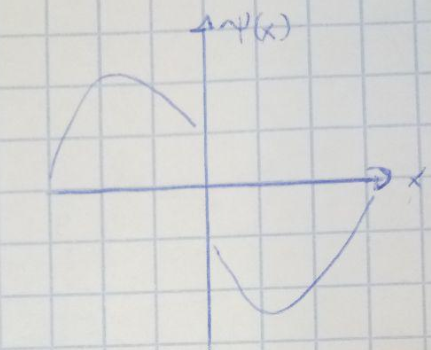
\includegraphics[width=.5\textwidth]
			{images/TipoI.png}
			\caption{esempio di regione}}
	\end{figure}
	\newpage
	
	\item $V(x)-E>0$
	
	\begin{align}
	V(x)>E \rightarrow  \frac{\psi''}{\psi}<0 \rightarrow 
	\left\{
	\begin{array}{cc}
	\psi''(x) >0 \, , \, \psi(x)>0 \\
	\psi''(x) <0 \, , \, \psi(x)<0
	\end{array}
	\right.
	\end{align}
	
	E si parla di  \textbf{regioni di tipo II}:
	
	\begin{figure}[!htb]
		\center{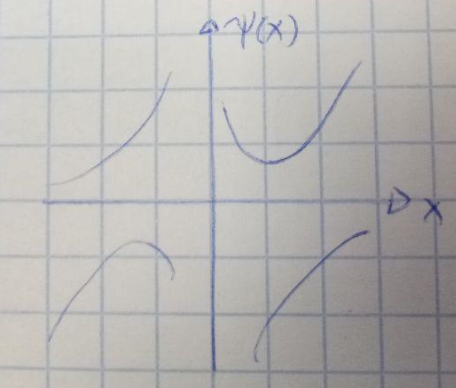
\includegraphics[width=.5\textwidth]
			{images/TipoII.png}
			\caption{esempio di regione}}
	\end{figure}
	
	
	\item $V(x)=E$ 

	  Si parla qui di \textbf{punti di inversione} da tipo I a tipo II e viceversa.
\end{enumerate}

\newpage

\subsection{Soluzioni dell'equazione di Schrödinger}

\subsubsection{Autovalori discreti}

Studiamo un sistema dove $\lim_{x \rightarrow \pm \infty}V(x)= +\infty$

Ci torveremo con due casi:

\begin{enumerate}
	\item $E<V_{\text{min}}$
	
	In questo caso $E<V(x) \; \forall x$, e si avranno quindi solo regioni di tipo II, con conseguente assenza di spettro discreto.
	
	\item $E>V_{\text{min}}$

	In questo caso ci troviamo ad avere entrambe le regioni

		\begin{align}
			\left\{
			\begin{array}{cc}
				E> V(x) \quad x \in [x_1 , x_2] \quad \text{tipo I }\\
				E< V(x) \quad x \notin [x_1 , x_2] \quad \text{tipo II}
			\end{array}
			\right.
		\end{align}

	e le nostre soluzioni si troveranno nelle regioni di tipo I.
\end{enumerate}

Le nostre soluzioni saranno tali che

\begin{align}
{}&\lim_{x \rightarrow \pm \infty} \psi(x)=0 \quad x \notin [x_1, x_2] \\
& \text{oppure} \nonumber \\
&\lim_{x \rightarrow \pm \infty} \psi(x)=\pm \infty \quad x \notin [x_1, x_2]
\end{align}

Ovvero nelle regioni di tipo II non può oscillare o rimanere limitata senza convergere a 0.

Cerchiamo di capire come ottenere soluzioni accettabili. 

Supponiamo di avere 

\begin{align}
\psi(x_0)>0 \quad ; \quad x_o<x_1
\end{align}

In questo caso ci basta fissare $\psi'(x_0)$ per risolvere il problema.

Ci troveremo con 3 casi:

\begin{enumerate}
	\item $\psi'(x_0)>0$ ma piccolo oppure $\psi'(x_0)<0$
	
	In questo caso avremo 
	\begin{align}
	\lim_{x \rightarrow -\infty}\psi(x)=+\infty \quad ; \quad \psi(x)\neq 0 \;\; \forall x
	\end{align}
	
	
	\item $\psi'(x_0)>0$ grande

	In questo caso avremo 
	\begin{align}
	\lim_{x \rightarrow -\infty}\psi(x)=-\infty \quad ; \quad \psi(x_a)= 0 \;\; x=x_a
	\end{align}
	
	\item $\psi'(x_0)>0$ nella media tra 1 e 2
	
	In questo caso avremo 
	\begin{align}
	\lim_{x \rightarrow -\infty}\psi(x)=0 \quad ; \quad \psi(x) \neq 0 \;\; \forall x
	\end{align}
		
\end{enumerate}

Ovviamente il tipo di soluzioni che fanno comodo a noi sono quelle del tipo 3.

Supponiamo ora per semplicità che tutto l'intervallo $[x_1,x_2]$ sia una sola regione di tipo I, e vediamo come si comporta per $x\rightarrow +\infty$.

Dentro $[x_1,x_2]$ avremo un comportamento oscillante di $\psi(x)$.

\newpage

Qualora ci troviamo in una situazione tale per cui $E>V(x)$ ma di poco, La $\psi(x)$ non si annulla mai, e avremo tre casi:

\begin{enumerate}
	\item $\lim_{x \rightarrow +\infty}\psi(x)=+\infty$
	
	\begin{figure}[!htb]
		\center{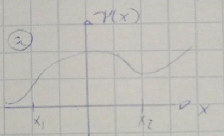
\includegraphics[width=0.3\textwidth]
			{images/I.png}
			\caption{\label{fig:my-label}}}
	\end{figure}
	In questo caso E non sarà autovalore valido, non essendo $\psi(x)$ a supporto compatto, e avremo $E_1<E_2$

	\item $\lim_{x \rightarrow +\infty}\psi(x)=0$

	\begin{figure}[!htb]
		\center{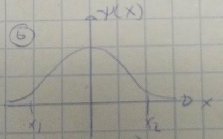
\includegraphics[width=0.3\textwidth]
			{images/II.png}
			\caption{\label{fig:my-label}}}
	\end{figure}
	In questo caso invece abbiamo invece una soluzione valida, a cui corrisponderà un valore ben distinto.
	
	\item $\lim_{x \rightarrow +\infty}\psi(x)=-\infty$

	\begin{figure}[!htb]
		\center{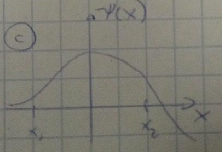
\includegraphics[width=0.3\textwidth]
			{images/III.png}
			\caption{\label{fig:my-label}}}
	\end{figure}

	Anche qui non abbiamo una soluzione valida per lo stesso motivo di 1, con $E_3>E_2$.
\end{enumerate}


Ricordando che 

\begin{align}
\psi''(x) = \frac{2m}{\hbar^2}(V(x)-E)\psi(x)
\end{align}


Notiamo come partendo da $E=V_{min}$ e incrementando valori di $E$ si passerà con continuità dal caso 1 al caso 3, e nel mezzo ci sarà sempre un insieme discreto che restituisce soluzioni accettabili.

Un'altra conseguenza è che l'autofunzione corrispondete al valore più basso di E non si annulla mai al finito, e quindi \textbf{non ha nodi}.

Aumentando l'energia si spostano i punti di inversione $x_1$ e $x_2$ rispettivamente a sinistra e a destra, e aumenta la curvatura di $\psi(x)$ all'interno, e conseguentemente il numero di volte che la funzione oscilla (ovvero attraversa l'asse x).

\newpage

Il fatto che le autofunzioni degli stati eccitati debbano avere nodi viene da fatto che 

\begin{align}
\int \psi_0(x)\psi_n(x)=0
\end{align}

e visto che $\psi_0(x)>0 \, \forall x$ per forza di cose devono potersi annullare, e quindi avere nodi le altre. QUesto ci porta ad enunciare il

\bigskip

\textbf{Teorema dei nodi:} 

\textit{Per un sistema con un solo grado di libertà e spettro discreto:}

\smallskip

$H\psi_0(x)= E_0\psi_0(x)$

$H\psi_1(x)= E_0\psi_1(x)$

...

$H\psi_n(x)= E_n\psi_n(x)$
\smallskip

\textit{Il numero di nodi di $\psi_n(x)$ viene dato dal numero quantico principale $n$.}

\bigskip

L'ultimo problema da risolvere per gli autovalori discreti è quello della degenerazione, che viene affrontato con il 


\textbf{Teorema della non degenerazione:}

\textit{Per ogni sistema 1D gli autovalori discreti della Hamiltoniana sono non degeneri.}

\bigskip

Questo si dimostra rapidamente prendendo in cosiderazione due autofunzioni qualsiasi $\psi_1(x)$ e $\psi_2(x)$ corrispondenti allo stesso autovalore $E$:

\begin{align}
\psi_1''(x) = \frac{2m}{\hbar^2}(V(x)-E)\psi_1(x) \\
\psi_2''(x) = \frac{2m}{\hbar^2}(V(x)-E)\psi_2(x)
\end{align}

Moltiplicando l'una per la $\psi(x)$ dell'altra e sottraendo membro a membro otteniamo che 

\begin{align}
\psi_1''(x)\psi_2(x) - \psi_1(x)\psi''_2(x)=0
\end{align}

che è uguale a scrivere

\begin{align}
\frac{\partial}{\partial x}(\psi_1'(x)\psi_2(x) - \psi_1(x)\psi'_2(x))=0
\end{align}

che, integrando porta a scrivere

\begin{align}
\psi_1'(x)\psi_2(x) - \psi_1(x)\psi'_2(x)= cost.
\end{align}

Ma $E$ è un autovalore discreto, e quindi le autofunzioni si annullano per $x \rightarrow \pm \infty$, e quindi $cost.=0$

questo ci porta a

\begin{align}
{}&\psi_1'(x)\psi_2(x) = \psi_1(x)\psi'_2(x) \\
&\downarrow \nonumber \\
&\frac{\psi_1'(x)}{\psi_1(x)}=\frac{\psi_2'(x)}{\psi_2(x)}\\
&\downarrow \nonumber \\
& \frac{\partial}{\partial x} \ln{\psi_1(x)} =  \frac{\partial}{\partial x}\ln{\psi_2(x)}
\end{align}

Integrando otteniamo che

\begin{align}
\psi_1(x) = C \psi_2(x)
\end{align}
e che quindi le due autofunzioni non sono indipendenti ed $E$ non è degenere.

Consideriamo ora un caso molto importante: $V(x)=V(-x)$

In questo caso avremo che $[H,I]=0$, e quindi ci sarà un insieme di autofunzioni simultanee.

Gli autovalori discreti $E$ sono non degeneri, e siccome ogni autofunzione di H corrispondente ad E è anche tale di $I$ deve avere anche parità definita.

Notiamo ora che

\begin{enumerate}
	\item Le funzioni \textbf{pari} hanno o un numero pari di nodi o infinito, in quanto se si annulla per dato $x_0$ si deve annullare anche a $-x_0$
	\item Le funzioni \textbf{dispari} hanno o un numero dispari di nodi o infinito, dovendosi annullare anche nell'origine per definizione, mentre se le pari se si annullano nell'origine hanno uno zero di ordine pari
\end{enumerate}

Però le soluzioni dell'eq di Schrödinger non possono avere zeri di ordine superiore al primo: se in un punto si annullano sia $\psi(x)$ che $\psi'(x)$ allora la soluzione è ben definita ed è quella identicamente nulla.

Ricordando anche il teorema dei nodi possiamo concludere dicendo che \textbf{la parità delle autofunzioni è data dal numero quantico principale $n$, con quella dello stato fondamentale sempre pari}.

\newpage

\subsubsection{Autovalori continui}

Consideriamo ora il seguente potenziale:

\begin{align}
\lim V(x)=
\left\{
\begin{array}{cc}
+\infty \quad x\rightarrow-\infty \\
0 \;\,\qquad x\rightarrow +\infty
\end{array}
\right.
\end{align}

	\begin{figure}[!htb]
	\center{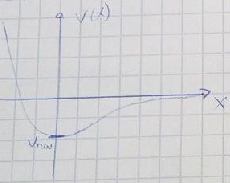
\includegraphics[width=0.3\textwidth]
		{images/contI.png}
		\caption{\label{fig:my-label}}}
\end{figure}

Ci troveremo a lavorare con tre casi:

	\begin{figure}[!htb]
	\center{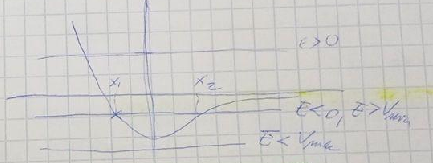
\includegraphics[width=0.3\textwidth]
		{images/contII.png}
		\caption{\label{fig:my-label}}}
\end{figure}

\begin{enumerate}
	\item $E<V_{min}$ 
	
	In questo caso tutto l'asse x  è una regione di tipo II e non sono ammessi autovalori.
	
	\item $V_{min}<E<0$ 
	
	In questo caso avremo solo autovalori discreti in una regione compresa tra due punti. Notiamo che per la forma del potenziale avremo la soluzione generale sarà della forma
	
	\begin{align}
	\alpha e^{\sqrt{sm|E|} \frac{x}{\hbar}} + \beta e^{-\sqrt{sm|E|} \frac{x}{\hbar}} \\
	\alpha, \beta \in \mathbb{C} \quad; \quad x\rightarrow +\infty
	\end{align}
	
	In questo caso, per $E$ fissato e scelta una soluzione che si annulla per $x\rightarrow -\infty$, di norma si ha una soluzione con entrambi i coefficienti $\neq 0$, ma è solo per quelle con $\alpha =0$ che si hanno soulzioni accettabili ed $E$ è autovalore di $H$.
	
	Il numero di autovalori dipende da $V(x)$. 
	
	In particolare \textbf{se $\lim_{x\rightarrow +\infty}V(x)\ll \lim_{x\rightarrow +\infty}x^{-2}$ e $V(x)$ limitata inferiormente allora  il numero di autovalori dell'energia sarà finito od eventualmente nullo}.
	
	\item $E>0$
	
	In questo caso per $x\ll 0$ avremo una regione di tipo II e per $x \gg 0$ saranno di tipo I. Sarà quindi possibile trovare una soluzione del tipo
	
	\begin{align}
	\alpha e^{i\sqrt{2mE} \frac{x}{\hbar}} + \beta e^{-i\sqrt{smE} \frac{x}{\hbar}} \\
	\alpha, \beta \in \mathbb{C} \quad; \quad x\rightarrow +\infty
	\end{align}
	
	E quindi sempre accetabile. Notiamo come al contrario dei casi precedentemente studiati non serve che la $\psi(x)$ si annulli per $x\rightarrow +\infty $, in quanto rimane comunque limitata. Abbiamo quindi che ogni $E>0$ è autovalore improprio di $H$ e ci troviamo in presenza di uno \textbf{spettro continuo}, in questo caso non degenere.
	\end{enumerate}

Un ultimo caso da considerare è il seguente:

\begin{align}
\lim V(x)=
\left\{
\begin{array}{cc}
V_1 \quad x\rightarrow -\infty \\
V_2 \quad x\rightarrow +\infty
\end{array}
\right. \quad ; \quad V_min<V_1<V_2
\end{align}

\begin{figure}[!htb]
	\center{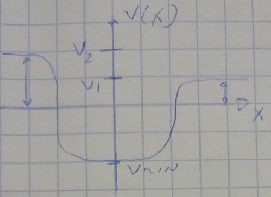
\includegraphics[width=0.5\textwidth]
		{images/contIII.png}
		\caption{\label{fig:my-label}}}
\end{figure}

Avremo qui 4 casi:

\begin{enumerate}
	\item $E<V_{min}$
	
	In questo caso non si hanno autovalori validi
	
	\item $V_{min}<E<V_1$
	
	Per $|x|\gg 0$ ho regioni di tipo II con in mezzo almeno una regione di tipo I, e quindi abbiamo solo autovalori discreti
	
	\item $V_1<E<V_2$
	
	Per $x \ll 0$ abbiamo una regione di tipo II, mentre per $x \gg 0$ ne avremo una di tipo I con tutti valori $E>0$, continui e non degeneri. È il caso speculare del caso 2 del precedente potenziale, e stavolta nella soluzione porremo $\beta=0$
	
	\item $E>V_2$
	
	Per $|x|\gg 0$ avremo regioni di tipo I, in mezzo dipende dalla forma di $V(x)$.
		Avremo 
	
	\begin{align}
	\psi(x)= \left\{
	\begin{array}{cc}
	\alpha e^{+i\frac{\sqrt{2m(E-V_2)}}{\hbar}}x + \beta e^{-i \frac{\sqrt{2m(E-V_2)}}{\hbar}x} \quad;\quad  x\rightarrow -\infty \\
	\gamma e^{+i \frac{\sqrt{2m(E-V_1)}}{\hbar}x} + \delta e^{-i \frac{\sqrt{2m(E-V_1)}}{\hbar}x} \quad;\quad  x\rightarrow +\infty \\
	\end{array}
	\right.
	\end{align}
	E tutte le soluzioni sono valide e per $E>V_2$ avremo uno spettro continuo 2 volte degenere, non essendo i coefficienti indipendenti.
\end{enumerate}

In generale si può dire che

\begin{enumerate}
	\item Tutto l'asse x di tipo II: no autovalori
	\item $x\rightarrow \pm \infty$ di tipo II: spettro discreto non degenere
	\item $x\rightarrow \pm \infty$ di tipo I $x\rightarrow \mp \infty$ di tipo II: spettro continuo non degenere
	\item $x\rightarrow \pm \infty$ di tipo I: spettro continuo 2 volte degenere
\end{enumerate}


\newpage
\section{L'oscillatore armonico (Caso 1D)}

L'oscillatore armonico viene descritto dall'Hamiltoniana:

\begin{align}
H = \frac{1}{2m} p^2  + \frac{1}{2} m \omega^2 q^2
\end{align}

Per la quale valgono le seguenti proprietà:

\begin{enumerate}
	\item i suoi autovalori sono tutti positivi, infatti, preso un $\ket{A}$ nomralizzato
	
	\begin{align}
	E=\overline{H}= \braket{A |H| A} \propto \braket{A |p^2| A}  + \braket{A |q^2| A} = |p \ket{A}|^2 +  |q\ket{A}|^2
	\end{align}
	
	essendo entrambi moduli sono entrambi $\geq 0$ per definizione, da cui segue che anche $\overline{H}$ lo è. Ma c'è un problema!
	
	\begin{align}
	E={}&\overline{H}=0 \rightarrow \braket{A |p^2| A}  + \braket{A |q^2| A} = 0 \nonumber \\
	&\downarrow\nonumber \\
	&\braket{A |p^2| A}  = -\braket{A |q^2| A} \nonumber \\
	&\downarrow\nonumber \\
	&\braket{A |p^2| A}  = \braket{A |q^2| A} = 0
	\end{align}
	
	Questo è impossibile, visto che $[q,p]=i\hbar$, questo implica che 
	
	\begin{align}
	E > 0
	\end{align}
	
	\item $\braket{A |q| A} = 0 = \braket{A |p| A}$
	
	 questo viene dimostrato dal fatto che
	 
	 \begin{align}
	 [V(q), q]=0 \rightarrow  [H,q]= \frac{1}{2m}[p^2,q]
	 \end{align}
	 ricordando le proprietà dei commutatori e la relazione di indeterminazione otteniamo
	 
	 \begin{align}
	 [p^2,q] = p[p,q] + [p,q]p= 2i\hbar p
	 \end{align}
	 
	 e quindi
	 \begin{align}
	 [H,q]= -\frac{i \hbar}{m}p
	 \end{align}
	 
	 calcolandone il valore medio su un autostato di H otteniamo
	 
	 \begin{align}
	 \braket{E_n|[H,q]|E_n} = \left\{
	 \begin{array}{cc}
		-\frac{i \hbar}{m}p \\
		\braket{E_n|Hq - qH|E_n}
	 \end{array}
	 \right.
	 \end{align}
	 
	 ma abbiamo anche che, ricordando che H è hermitiana,
	 \begin{align}
	{}&\braket{E_n|Hq - qH|E_n} = \braket{E_n|Hq|E_n} - \braket{E_n|qH|E_n} \\ 
	&\downarrow \nonumber \\
	&E_n\braket{E_n|q|E_n} - \braket{E_n|q|E_n}E_n=0
	 \end{align}

	da cui $\braket{E_n|p|E_n}=0$. Si dimostra allo stesso modo calcolando $[H,p]$ che anche $\braket{E_n|q|E_n}=0$.

\item $E_0 \geq \frac{1}{2} \hbar \omega$
	\begin{align}
	{}&\braket{E_0|E_0}=1 \\
	 &\downarrow \nonumber \\ 
	 &E_0= \braket{E_0|H|E_0}= \frac{1}{2m}\braket{E_0|p^2|E_0} + \frac{m\omega^2}{2}\braket{E_0|q^2|E_0} \\
	 &\downarrow \nonumber \\ 
	 &E_0=  \frac{1}{2m}(\Delta p)^2 + \frac{m\omega^2}{2}(\Delta q)^2 \geq \omega \Delta p \Delta q = \frac{1}{2}\hbar \omega
	 \end{align}
	 
	 l'ultimo passaggio è dovuto alla disuguaglianza triangolare e al principio d'indeterminazione.
\end{enumerate}

\subsection{Spettro e autovettori dell'oscillatore armonico}

Per descrivere lo spettro introduciamo gli operatori non hermitiani detti di \textbf{discesa} e \textbf{salita}:

\begin{align}
\eta = \frac{1}{\sqrt{2m\omega\hbar}}(p - im\omega q) \quad ; \quad \eta^\dagger =\frac{1}{\sqrt{2m\omega\hbar}}(p + im\omega q)
\end{align}

da cui ricaviamo

\begin{align}
q= -\i \sqrt{\frac{\hbar}{2m\omega}}(\eta^\dagger - \eta )  \quad ; \quad p = \sqrt{\frac{m\hbar\omega}{2}}(\eta^\dagger + \eta ) 
\end{align}

o, come si trova in altri testi come il Patrì-Testa (noi useremo la prima definizione, ma per completezza riportiamo anche questa):

\begin{align}
a= \sqrt{\frac{m\omega}{2\hbar}}(q+ \frac{i}{m\omega}p)\quad &; \quad a^\dagger = \sqrt{\frac{m\omega}{2\hbar}}(q- \frac{i}{m\omega}p) \\
q= \sqrt{\frac{\hbar}{2m\omega}}(a + a^\dagger) \quad &; \quad p= i\sqrt{\frac{m\omega \hbar}{2}}(a - a^\dagger)
\end{align}

Iniziamo calcolando quantità utili per le prossime dimostrazioni:

\begin{align}
\eta^\dagger \eta {}&= \frac{1}{2m\omega\hbar}[p^2 + (m\omega)^2 q^2 + im\omega(qp - pq)]= \nonumber \\
& = \frac{1}{2m\omega\hbar}(p^2 + (m\omega)^2 q^2 + im\omega[q,p])= \nonumber \\
&= \frac{1}{2m\omega\hbar}(p^2 + (m\omega)^2 q^2 + im\omega i\hbar)= \nonumber \\
&= \frac{1}{2m\omega\hbar}(p^2 + (m\omega)^2 q^2 - m\omega\hbar) = \nonumber \\
&= \frac{1}{\hbar\omega}\left(\frac{1}{2m}p^2 + \frac{m\omega^2}{2} q^2\right) - \frac{1}{2}= \frac{1}{\hbar\omega}H -\frac{1}{2} \\
\nonumber \\
\eta \eta^\dagger &= \frac{1}{\hbar\omega}H +\frac{1}{2}
\end{align}

\newpage 
Da cui otteniamo: 

\begin{align}
{}&H =\hbar\omega \, \eta^\dagger \eta + \frac{\hbar\omega}{2} \\
&[\eta,\eta^\dagger]=1 \\
&[H,\eta]= \hbar\omega [\eta^\dagger \eta, \eta]= -\hbar\omega \eta \\
&[H,\eta^\dagger]= \hbar\omega [\eta^\dagger \eta, \eta^\dagger]= \hbar\omega \eta
\end{align}

Vediamo ora perché il nome degli operatori introdotti. Iniziamo con quello di \textbf{discesa}:

\begin{align}
H\eta\ket{E_n} {}&= ([H,\eta] +\eta H)\ket{E_n}= (-\hbar\omega \eta + +\eta H)\ket{E_n}= \nonumber \\
&= -\hbar\omega \eta \ket{E_n} + \eta H \ket{E_n} = -\hbar\omega \eta \ket{E_n} + \eta E_n \ket{E_n}=\nonumber \\
&=  (E_n-\hbar \omega) \eta \ket{E_n}
\end{align}

Notiamo come $\eta \ket{E}$ sia ancora autovalore di H, ma di un livello ad energia più bassa!

considerando il terzo punto dello scorso paragrafo, dovremo avere un'energia minima, che troviamo nel seguente modo: 

\begin{align}
{}&E \geq 0 \rightarrow \exists E_0: \eta \ket{E_0}=0 \\
&\downarrow \nonumber \\
&0=\bra{E_0}\eta^\dagger\eta \ket{E_0} = \braket{E_0|\frac{1}{\hbar\omega}H -\frac{1}{2}|E_0}= \frac{1}{\hbar\omega}E_0 -\frac{1}{2} \nonumber\\
&\downarrow \nonumber \\
& E_0= \frac{1}{2}\hbar\omega
\end{align}

Mentre invece non c'è un valore massimo possibile, infatti

\begin{align}
{}&0=\bra{E_{max}}\eta\eta^\dagger \ket{E_{max}} = \braket{E_{max}|\frac{1}{\hbar\omega}H +\frac{1}{2}|E_{max}}= \frac{1}{\hbar\omega}E_{max}+\frac{1}{2} \nonumber\\
&\downarrow \nonumber \\
& E_{max}= -\frac{1}{2}\hbar\omega
\end{align}

che è impossibile. 
 
Possiamo quindi ricavare lo spettro, applicando n volte $\eta^\dagger$ a $E_0$, ottenendo

\begin{align}
E_n= \left(\frac{1}{2}+n\right)\hbar\omega
\end{align}

Notiamo anche che che

\begin{align}
E_n-\hbar \omega = \left(\frac{1}{2}+n - 1\right)\hbar\omega \\
E_n+\hbar \omega = \left(\frac{1}{2}+n + 1\right)\hbar\omega
\end{align}

\newpage
Da cui segue che, chiamati gli autovettori $\ket{n}$

\begin{align}
\eta \ket{n}=\sqrt{n}\ket{n- 1}\\
\eta^\dagger  \ket{n}= \sqrt{n+1}\ket{n+ 1}
\end{align}

Definiamo così gli autostati normalizzati

\begin{align}
\ket{n}= \frac{(\eta^\dagger)^n}{\sqrt{n!}}\ket{0}
\end{align}


\subsection{L'oscillatore armonico 1D in RS}

Come possiamo esprimere l'oscillatore armonico in uno spazio $L_2$?

Una via è la risoluzione dell'equazione di Schrödinger:

\begin{align}
-\frac{\hbar^2}{2m}\psi_n''(x)+\frac{m\omega^2x^2}{2}\psi_n(x)=E_n\psi_n(x) 
\end{align}

Ma c'è una via più semplice! Infatti abbiamo che

\begin{align}
{}&\ket{n}= \frac{(\eta^\dagger)^n}{\sqrt{n!}}\ket{0} \rightarrow \psi_n(x)= \braket{x|n}= \frac{(-1)^n}{\sqrt{n!}}\braket{x|\eta^\dagger|0} \\
\nonumber \\
&\eta^\dagger = \frac{1}{\sqrt{2m\omega\hbar}}(p + im\omega q) \rightarrow \eta^\dagger= \frac{1}{\sqrt{2m\omega\hbar}} \left( -i\hbar \frac{\partial}{\partial x} + im\omega x \right)
\end{align}

Da cui ricaviamo

\begin{align}
\psi_n(x)= \frac{(2m\omega \hbar)^{\frac{n}{2}}}{\sqrt{n!}}\left( -\hbar \frac{\partial}{\partial x} + m\omega x \right)^n \psi_0(x)
\end{align}


ma come troviamo $\psi_0(x)$?

Ricordando che $\ket{0}: \eta\ket{0}=0$ avremo

\begin{align}
\left( \hbar \frac{\partial}{\partial x} + m\omega x \right) \psi_0(x) =0
\end{align}

Che è un'eqauzione differenziale al primo ordine che possiamo risolvere senza problemi!

\begin{align}
{}&\hbar \psi'_0(x) + m\omega x \psi_0(x)=0 \nonumber \\
& \downarrow \nonumber \\
& \frac{\partial \psi_0(x)}{\psi_0(x)} = -\frac{m\omega}{\hbar} x \partial x  \nonumber \\
& \downarrow \nonumber \\
& \int_{\psi_0(0)}^{\psi_0(x)} \frac{\partial \psi_0(x)}{\psi_0(x)} = -\frac{m\omega}{\hbar} \int_{0}^{x} \partial x \; x  \nonumber \\
& \downarrow \nonumber \\
& \ln(\frac{\psi_0(x)}{\psi_0(0)}) = -\frac{m\omega}{2\hbar}x^2 \nonumber \\
& \downarrow \nonumber \\
& \psi_0(x) = \psi_0(0) e^{-\frac{m\omega}{2\hbar}x^2}
\end{align}

(nota: chiamare gli estremi di integrazione e la variabile di integrazione con lo stesso nome è un vizio di forma per non confondere il lettore introducendo troppe variabili).

Per trovare $\psi_0(0)$ ci basta normalizzare:

\begin{align}
{}&|\psi_0(x)|^2 = 1 = \int_{-\infty}^{+\infty} |\psi_0(0)|^2 e^{-\frac{m\omega}{\hbar}x^2} \nonumber \\
& \downarrow \nonumber \\
&1=|\psi_0(0)|^2 \int_{-\infty}^{+\infty}  e^{-\frac{m\omega}{\hbar}x^2} = |\psi_0(0)|^2 \sqrt{\frac{\hbar \pi}{m \omega}}\nonumber \\
& \downarrow \nonumber \\
&|\psi_0(0)|^2 \sqrt{\frac{\hbar \pi}{m \omega}}=1 \rightarrow \psi_0(0)= \sqrt[4]{\frac{\hbar \pi}{m \omega}}
\end{align}

E possiamo quindi scrivere

\begin{align}
\psi_0(x) = \sqrt[4]{\frac{\hbar \pi}{m \omega}} e^{-\frac{m\omega}{2\hbar}x^2}
\end{align}

In conclusione scriviamo quindi

\begin{align}
\psi_n(x)= \frac{(2m\omega \hbar)^{-\frac{n}{2}}}{\sqrt{n!}}\left( -\hbar \frac{\partial}{\partial x} + m\omega x \right)^n \sqrt[4]{\frac{\hbar \pi}{m \omega}} e^{-\frac{m\omega}{2\hbar}x^2}
\end{align}

Possiamo anche scrivere il tutto in modo più compatto introducendo i \textbf{polinomi di Hermite}:

\begin{align}
H_n(\xi) = e^{\frac{\xi^2}{2}} \left( -\frac{\partial}{\partial \xi} + \xi \right)^n e^{-\frac{\xi^2}{2}}
\end{align}

e ponendo $\xi = \sqrt{-\frac{m\omega}{2\hbar}}x$, ottenendo in conclusione:

\begin{align}
\psi_n(x)= \frac{1}{\sqrt{2^n n!}}\sqrt[4]{\frac{\hbar \pi}{m \omega}}H_n\left(\sqrt{-\frac{m\omega}{2\hbar}}x\right) e^{-\frac{m\omega}{2\hbar}x^2}
\end{align}

\newpage

\section{L'oscillatore armonico (Caso 3D)}

Nel caso 3D H assume la forma

\begin{align}
H= \frac{1}{2m}p^2 + \frac{m\omega^2}{2}q^2 \quad;\quad 
\left\{
\begin{array}{cc}
p^2= p_x^2 + p_y^2 + p_z^2 \\
q^2= x^2 + y^2 + z^2
\end{array}\right.
\end{align}

In questo caso V(q) fa parte della famiglia dei \textbf{potenziali centrali}, che studiamo nel prossimo capitolo, e quindi come vederemo gli autovettori ed autofunzuoni potranno essere espresse come
\begin{align}
\ket{E,l,m} \leftrightarrow \psi_{elm}(q)
\end{align}

Invece di risolvere l'equazione di Schrödinger, che richiederebbe numerosi conti, possiamo riscrivere H \textbf{separando le variabili}!

\begin{align}
H{}&=\left(\frac{1}{2m} p_x^2  + \frac{m \omega^2}{2}  x^2 \right) + \left(\frac{1}{2m} p_y^2  + \frac{m \omega^2}{2}  y^2 \right) + \left(\frac{1}{2m} p_z^2  + \frac{m \omega^2}{2}  z^2 \right) \nonumber = \\
&= H_x + H_y + H_z
\end{align}

Da cui segue che 

\begin{align}
E{}& = E_x + E_y + E_z = \left( \frac{1}{2}+ \frac{1}{2}+\frac{1}{2} + n_x + n_y + n_z \right) \hbar \omega=\nonumber \\
&= \left(\frac{3}{2} + n_{3D}\right)\hbar \omega
\end{align}

E quindi possiamo anche esprimere le autofunzioni come 

\begin{align}
\ket{n_x, n_y, n_z} \leftrightarrow \psi_{n_x, n_y, n_z}(x,y,z)
\end{align}

con

\begin{align}
\psi_{n_x, n_y, n_z}(x,y,z) {}&= \psi_{n_x}(x) \psi_{n_y}(y) \psi_{n_z}(z)= \nonumber \\ 
&=\tilde{H}_{n_x}(x)\tilde{H}_{n_y}(y)\tilde{H}_{n_z}(z)e^{-\frac{m\omega}{2\hbar}r^2}
\end{align}

\begin{align}
\tilde{H}_{n_{q_i}}(q_i) = H_{n_{q_i}}\left( \sqrt{\frac{m\omega}{\hbar}} q_i\right) \quad ; \quad r^2 = x^2 + y^2 + z^2
\end{align}

E avremo che la degenerazione di ogni stato sarà data da

\begin{align}
g_{n_{3D}}= \frac{(n_{3D} + 1)(n_{3D} + 2)}{2}
\end{align}

Ora dobbiamo però porci il problema di come si passa da$\left\{n_x, n_y, n_z\right\}$ a $\left\{E,l,m\right\}$.

\begin{enumerate}
	\item Lo stato fondamentale $n_{3D}=0$ 
	
	$\ket{0,0,0}$
	
	Questo sarà non degenere e per forza uno stato con $l=0$, essendo uno stato simmetrico privo di nodi, definito come (a meno di costanti)
	\begin{align}
	\psi_{000}(x,y,z)\propto e^{-\frac{m\omega}{2\hbar}r^2} \nonumber
	\end{align}
	
	\item Io stato eccitato $n_{3D}=1$ 
	
	$\ket{1,0,0}$, $\ket{0,1,0}$, $\ket{0,0,1}$
	
	È un livello 3 volte degenere, e o si ha tre volte $l=0$ o si ha $l=1$ con $l_z= 0,\pm 1$. Il primo si esclude perché, come abbiamo visto in precedenza, \textbf{essendo $n_{3D}=1$ dispari, non possiamo avere uno stato pari}.
	
	\newpage
	
	\item IIo stato eccitato $n_{3D}=2$ 
	
	$\ket{1,1,0}$, $\ket{1,0,1}$, $\ket{0,1,1}$
	
	$\ket{2,0,0}$, $\ket{0,2,0}$, $\ket{0,0,2}$
	
	In questo caso abbiamo degenerazione pari a 6. Abbiamo due opzioni:
	
	\begin{enumerate}
		\item $l=0$ sei volte, il che è impossibile, non essendo alcuno degli stati a simmetria sferica (minimo 1 nodo ognuna).
		
		\item 
		\begin{enumerate}
			\item $l_1=0 \quad ; \quad l_{z_1}=0$
			\item $l_2=2  \quad ; \quad l_{z_2}=0,\pm 1, \pm 2$
		\end{enumerate}
		Però c'è un problema: \textbf{qual è lo stato corrispondente a $l_1=0$?}
		
		I tre stati $\ket{1,1,0}$, $\ket{1,0,1}$, $\ket{0,1,1}$ sono tutti corrispondenti ad $l_2=2$, ortogonali a $Y^0_0$ con autofunzioni del tipo
		\begin{align}
		\psi_{110}(x,y,z)\propto xy e^{-\frac{m\omega}{2\hbar}r^2} \propto r^2 \sin^2{\theta} \sin{2\phi} \,e^{-\frac{m\omega}{2\hbar}r^2} \nonumber
		\end{align}
		
		Gli altri tre stati $\ket{2,0,0}$, $\ket{0,2,0}$, $\ket{0,0,2}$ sono invece combinazioni di stati tra $l_1=0$ e $l_2=2$, e dato che $\tilde{H}_2(x) \propto x^2 + a$ avremo
		
		\begin{align}
		\psi_{200} + \psi_{020} + \psi_{002} \propto (x^2 + y^2 + z^2 + 3a)e^{-\frac{m\omega}{2\hbar}r^2} \nonumber
		\end{align}
		
		Che è simmetria sferica, e quindi associabile a $l_1=0$, e quindi scriviamo
		\begin{align}
		\ket{E_2, l=0}= \ket{2,0,0} + \ket{0,2,0} + \ket{0,0,2} \nonumber
		\end{align}
		\end{enumerate}
\end{enumerate}

E così via salendo. In generale il livello $n$-esimo avrà $l=n,n-2,...$ fino a $0$ o $1$ a seconda di $n$ pari o dispari.
 
\newpage

\section{La buca di potenziale (caso 1D)}

 Si chiamano buche di potenziale i sistemi descritti da
 
 \begin{align}
  H= \frac{1}{2m} p^2 + V(x) \quad;\quad V(x)= \left\{
  \begin{array}{cc}
V_0 \quad x \notin [-a,a]\\
0 \quad \;\: x \in [-a,a]
 \end{array}
  \right.
 \end{align}
 
  \begin{figure}[!htb]
  	\center{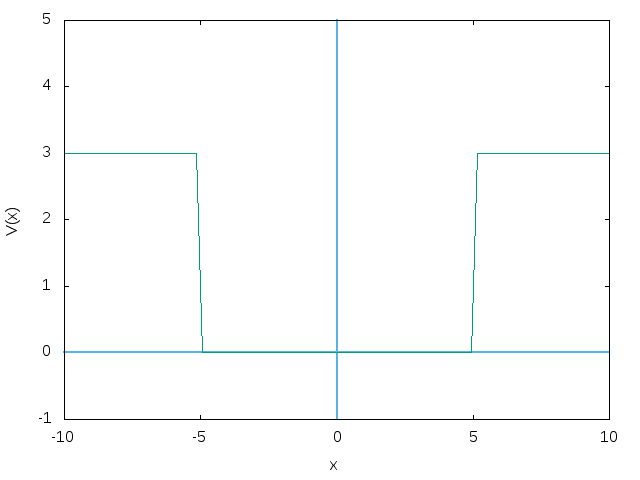
\includegraphics[width=0.7\textwidth]
  		{images/buca.png}
  		\caption{\label{fig:my-label2} esempio di buca simmetrica}}
  \end{figure}
 
 \textbf{Nota bene:} qui abbiamo posto gli estremi della buca simmetrici rispetto all'asse y e $V_0$ positivo, ma uno degli estremi potrebbe tranquillamente essere posto su $x=0$, cambierebbe solo il calcolo delle autofunzioni per questioni di simmetria, come vedremo più avanti. In casi diversi (ex. una buca con $V(x)\neq 0 \; \forall x \in[c,d]$ entrambi maggiori di 0) è sempre possibile applicare cambi di variabile per ricondursi ai primi due casi, decisamente più comodi da studiare.
  
 Che forma avranno le autofunzioni? Prima di risolvere l'equazione di Schrödinger, studiamo la continuità. Sappiamo che:
 
 \begin{align}
 \psi''(x)= \frac{2m}{\hbar^2}[V(x)-E]\psi(x) \\
 \downarrow \nonumber \\
 \psi'(\epsilon) - \psi'(0)= \frac{2m}{\hbar^2} \int_{0}^{\epsilon}dx [V(x)-E]\psi(x)
  \end{align}
 
 
 Siccome $V(x), \, \psi(x)$ sono limitate in $(0,\epsilon)$ avremo che il secondo termine $\rightarrow 0$ per $\epsilon \rightarrow 0$ da cui segue che
 
 \begin{align}
 \lim_{\epsilon \rightarrow 0}\psi'(\epsilon)= \psi'(0)
 \end{align}
 
 Quindi $\psi'(x)$ è continua ai bordi, e per conseguenza lo è anche $\psi(x)$.
\newpage 
 Studiamo ora l'eq. di Schrödinger nel caso di buca simmetrica:
 
 \begin{align}
 \psi''(x)=
 \left\{
\begin{array}{cc}
\frac{2mE}{\hbar}{}&\psi(x)\quad x\in [-a,a] \\
\frac{2m(V_0 - E)}{\hbar}&\psi(x) \quad x\notin [-a,a]
\end{array} 
 \right.
 \end{align}
 
per pulizia definiamo

\begin{align}
{}&k= \frac{\sqrt{2mE}}{\hbar} \\
&K= \frac{\sqrt{2m(V_0 - E)}}{\hbar}
\end{align}

Iniziamo studiando le \textbf{soluzioni pari}:

\begin{align}
 \psi_p(x)=
 \left\{
 \begin{array}{ccc}
 A\cos{kx}+ A'\sin{kx} \quad {}&x\in [-a,a] \\
 Be^{-Kx}+B'e^{+Kx} \quad &x>+a \\
 Ce^{+Kx}+C'e^{-Kx} \quad &x<-a
 \end{array} 
 \right.
\end{align}
 
Ricordando che $\psi(x)\in L_2$ abbiamo che
\begin{align}
B'= C'=0
\end{align}
e dal fatto che stiamo studiando le soluzioni pari ne segue che

\begin{align}
A'=0
\end{align}

E quindi in conclusione

\begin{align}
\psi_p(x)=
\left\{
\begin{array}{ccc}
A\cos{kx} \quad {}&x\in [-a,a] \\
Be^{-Kx} \quad &x>+a \\
Be^{-Kx} \quad &x<-a
\end{array} 
\right.
\end{align}

Siccome $\psi(x)$ è continua avremo anche che, per $x=a$ (discorso analogo per l'altro estremo):

\begin{align}
{}&\psi(a)\rightarrow A\cos{ka}= Be^{-Ka} \\
&\psi'(a)\rightarrow Ak\sin{ka}= KBe^{-Ka}
\end{align}

le cui soluzioni vengono da

\begin{align}
{}&A=B=0 \; \text{(soluzione banale)}\\
&k\tan{ka}=K
\end{align}


\newpage
Per le soluzioni dispari avremo invece

\begin{align}
\psi_d(x)=
\left\{
\begin{array}{ccc}
A\sin{kx} \quad {}&x\in [-a,a] \\
+Be^{-Kx} \quad &x>+a \\
-Be^{+Kx} \quad &x<-a
\end{array} 
\right.
\end{align}

con soluzioni

\begin{align}
{}&A=B=0 \; \text{(soluzione banale)}\\
&\frac{k}{\tan{ka}}=-K
\end{align}
 
di nuovo, per pulizia di notazione, definiamo

\begin{align}
\xi=ka \\
\eta= Ka
\end{align}

e possiamo ora scrivere che

\begin{align}
{}&\eta_p= \xi \tan{\xi} \quad \; \text{soluzioni pari} \\
&\eta_d= -\frac{\xi}{\tan{\xi}}  \quad \text{soluzioni dispari}
\end{align}

e possiamo infine ricavare le soluzioni degli stati legati, che ricaviamo dalle intersezioni di $\eta_p$ e $\eta_d$ con

\begin{align}
\xi^2 + \eta^2 = \frac{2mV_0a^2}{\hbar^2}
\end{align}

*INSERIRE GRAFICO*

si nota come il numero di stati legati sia finito. Ad esempio se

\begin{align}
\frac{2mV_0a^2}{\hbar^2} <\frac{\pi^2}{4}
\end{align}

avremo solo uno stato pari, e per averne almeno uno dispari bisogna andare oltre $\frac{\pi^2}{4}$.

\newpage

\subsection{Caso di buca infinita}

Si parla di buca infinita quando il potenziale ha forma

\begin{align}
V(x)= \left\{
\begin{array}{cc}
0 \quad {}&x \in [-a,a]\\
+\infty  &x \notin [-a,a]
\end{array}
\right.
\end{align}

In questo caso, guardando il grafico precedente, notiamo che

\begin{align}
ka \rightarrow \frac{\pi}{2}
\end{align}

da cui le soluzioni prendono la forma

\begin{align}
\psi(x)=
\left\{
\begin{array}{ccc}
A\cos{kx} \quad {}& x\in [-a,a] \\
+Be^{-K(x-a)} \quad &x>+a \\
-Be^{+K(x+a)} \quad &x<-a
\end{array} 
\right.
\end{align}

Ma $\cos{\frac{\pi}{2}}=0$, e quindi

\begin{align}
\psi(x)=
\left\{
\begin{array}{ccc}
A\cos{\frac{\pi x}{2a}} \quad {}& x\in [-a,a] \\
0 &x\notin [-a,a]
\end{array} 
\right.
\end{align}

Studiamo le soluzioni dentro la buca. Prendiamo una buca $[0,a]$ e imponiamo

\begin{align}
\left\{
\begin{array}{ccc}
\psi_n(a)= \psi_n(-a)=0\\
V_0=+\infty \qquad \qquad \;\,\\
|x|>a \quad \qquad \qquad \;\;
\end{array} 
\right.
\end{align}

Questo significa che presa

\begin{align}
\psi''(x)= \frac{2mE}{\hbar^2}\psi(x) \rightarrow \psi(x)= A\sin{kx}+B\cos{kx}
\end{align}

considerando le condizioni ai bordi, e al fatto che è buca antisimmetrica bisogna porre

\begin{align}
\psi(a)=\psi(0)=0 \quad ; \quad B=0
\end{align}

da cui

\begin{align}
A\sin{ka}=0 \rightarrow ka=n\pi \rightarrow k = \frac{n\pi}{a} \quad ; \quad n>0
\end{align}

e quindi per buche antisimmetriche si ottiene

\begin{align}
{}&\psi_n(x)= A\sin{\frac{n\pi x}{a}} \\
&ka=n\pi \rightarrow \frac{\sqrt{2mE_n}}{\hbar}a= n\pi \rightarrow \frac{2mE_n}{\hbar^2}a^2= n^2\pi^2 \nonumber \\
&\downarrow \nonumber\\
&E_n= \frac{\hbar^2 \pi^2}{2ma^2}n^2
\end{align}

Mentre per le simmetriche (del tipo $ [-a,a]$) basta sostituire il seno col coseno.

\newpage

\section{Barriera di potenziale ed effetto tunnel}

Si parla di barriera di potenziale quando si ha un sistema del tipo

\begin{align}
V(x)= \left\{
\begin{array}{ccc}
0 \quad {}&x\notin[0,L]\\
V_0\quad &x\in[0,L]
\end{array} 
\right.
\end{align}

\begin{figure}[!htb]
	\center{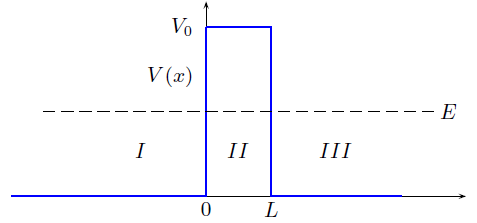
\includegraphics[width=0.6\textwidth]
		{images/BP.png}
		}
\end{figure}

Classicamente parlando, tutte le particelle con $E<V_0$ provenienti da ambo i lati verrebbero semplicemente riflesse indietro. Quantisticamente ciò non è detto, e si parla di \textbf{effetto tunnel}.

Questo perché le regioni ai lati della barriera sono di tipo I, e hanno quindi autovalori continui e discreti, da cui

\begin{align}
\psi(x)=\left\{
\begin{array}{cc}
Ae^{ikx} + A'e^{-ikx} 	\quad x\leq 0\\
Ce^{ikx} + C'e^{-ikx} 	\quad x\geq a
\end{array}
\right.
\end{align}

Siccome l'eq. di Schrödinger è di 2o grado, solo due dei coefficienti di $\psi(x)$ saranno linearmente indipendenti, a seconda della direzione della particella.

Studiamo il problema con una particella che arriva da sinistra. In questo caso, affinché la soluzione sia limitata deve essere

\begin{align}
A\neq 0 \quad;\quad C'=0
\end{align}

\begin{align}
\psi(x)=\left\{
\begin{array}{cc}
e^{ikx} + A'e^{-ikx} 	\quad {}&x\leq 0\\
Ce^{ikx}  \qquad \quad \; \; 	\quad &x\geq a
\end{array}
\right.
\end{align}


Deve essere $C\neq 0$ perché le soluzioni non poso annullarsi con la derivata in un punto, figuriamoci in un intervallo, mentre $A=1$ è dovuto all'omogeneità dell'equazione.

Come possiamo vedere \textbf{è possibile che la particella si trovi a destra della barriera, pur venendo da sinistra}.

Nell'ottica della barriera di potenziale possiamo dare i seguenti nomi ai coefficienti

\begin{align}
|A|^2=1 \qquad {}&\text{Coefficiente di incisione} \\
|A'|^2 \qquad \quad \;\; &\text{Coefficiente di riflessione} \\
|C|^2  \qquad \quad \;\;\, &\text{Coefficiente di trasmissione}
\end{align}

A' e C dipendono dal potenziale, ma vale sempre la relazione 

\begin{align}
|A'|^2+|C|^2=1
\end{align}

Per dimostrarlo partiamo dal caso 3D:

\begin{align}
-\frac{\hbar^2}{2m}\Delta \psi + V \psi= E \psi \quad;\quad \Delta = \nabla^2= \left(
\frac{\partial^2}{\partial x^2} + \frac{\partial^2}{\partial y^2} + \frac{\partial^2}{\partial z^2}
\right)
\end{align}

Considerata la coniugata:


\begin{align}
-\frac{\hbar^2}{2m}\Delta \psi^* + V \psi^*= E \psi^*
\end{align}

Moltiplichiamo prima l'una per l'altra e viceversa e sottraiamo i due risultati, ottenendo:

\begin{align}
\psi^*\Delta \psi - \psi \Delta \psi^*=0 \rightarrow \text{div}(\psi^*\Delta \psi - \psi \Delta \psi^*)=0
\end{align}

Definiamo la \textbf{corrente di probabilità} come:

\begin{align}
j = -\frac{i\hbar}{2m}(\psi^*\Delta \psi - \psi \Delta \psi^*)
\end{align}

da cui, se $\psi=\psi^*$ otteniamo l'\textbf{equazione di continuità}:

\begin{align}
\text{div} j = 0
\end{align}

Che ci porta ad avere, nel caso 1D:

\begin{align}
\frac{\partial}{\partial x}(\psi^*\Delta \psi - \psi \Delta \psi^*)= 0
\end{align}


Integrando su di un intervallo $[x_1,x_2]$ si ottiene

\begin{align}
\text{Im}(\psi^*(x_1)\psi'(x_1))=\text{Im}(\psi(x_2)\psi'x^*(x_2))
\end{align}

Qualora $x_1 <0 \, ,\, x_2>a$ risulta

\begin{align}
{}&\text{Im}[(e^{-ikx_1} + Ae^{-ikx_1})   (ike^{ikx_1} -ikA e^{-ikx_1})] = \text{Im}[Ce^{ikx_2}(-i)kCe^{-ikx_2}] \nonumber \\
&\downarrow \nonumber \\
&\text{Im}[ik - ikA e^{-2ikx_1} + ikA e^{-2ikx_1} -ik |A|^2 ] = \text{Im}[C(-i)kC] \nonumber \\
&\downarrow \nonumber \\
& \text{Im}[ik -ik |A|^2 ] = \text{Im}[-ik|C|^2]\nonumber \\
&\downarrow \nonumber \\
& \text{Im}[ik(1 -|A|^2) ] = \text{Im}[-ik|C|^2]\nonumber \\
&\downarrow \nonumber \\
& 1- |A|^2=|C|^2 \rightarrow |A|^2+|C|^2=1
\end{align}


Svolgendo conti che in queste dispense NON faremo perché mi rifiuto CATEGORICAMENTE è possibile ricavare il valore di $|C|^2$, che riportiamo di seguito:

\begin{align}
|C|^2 = \frac{4E(V_0 - E)}{4E(V_0 - E) - V_0^2 \sinh{Ka}} \quad;\quad K= \frac{\sqrt{2m(V_0 - E)}}{\hbar}
\end{align}



\chapter{Equazione di Schrödinger nel caso 3d e potenziali centrali}

\section{Equazione di Schrödinger nel caso 3d}

Trascurando eventuali dipendenze temporali, possiamo scrivere

\begin{equation}
\hat H \psi(\underline r)= \left(
\frac{\hat p^2}{2m} + V(\underline r)
\right)\psi(\underline r)= E\psi(\underline r)
\end{equation}

Essendo ora in 3d avremo che

\begin{align}
\hat{\underline p} = -i\hbar \left(
\frac{\partial}{\partial x}, \frac{\partial}{\partial y}, \frac{\partial}{\partial z}
\right) \rightarrow 
\hat{p^2} = -\hbar^2 \left(
\frac{\partial^2}{\partial x ^2} + \frac{\partial^2}{\partial y^2} + \frac{\partial^2}{\partial z^2}
\right) = - \hbar^2 \nabla^2
\end{align}

da cui otteniamo

\begin{align}
 \frac{\hbar^2}{2m} \nabla^2\psi(x,y,z) - [V(x,y,z) - E]\psi(x,y,z)=0
\end{align}

Ma come si studia questo problema? In alcuni casi è possibile studiare il problema nel caso 1d lungo gli assi per poi sommare i contributi, e in questo caso si parla di \textbf{metodo della separazione di variabili}:

\begin{equation}
H(x,y,z)= H(x) + H(y) + H(z)
\end{equation}


Esempi di sistemi che rientrano in questa categoria sono
\begin{enumerate}
	\item la buca di potenziale a parallelogramma (la "scatola")
	\item l'oscillatore armonico 3d (isoptropo e anisotropo)
\end{enumerate}

Qualora non sia possibile il problema si complica.

\newpage

\section{Potenziali centrali}

Si definiscono tali i potenziali tali che

\begin{equation}
V(r,\theta,\phi) \neq V(r)
\end{equation}

Per studiare questo genere di problemi ci conviene passare in coordinate sferiche. Scriviamo quindi:

\begin{align}
\nabla^2 {}&= \frac{\partial^2}{\partial x ^2} + \frac{\partial^2}{\partial y^2} + \frac{\partial^2}{\partial z^2}  \nonumber \\
&\downarrow \nonumber \\
\nabla^2 &=\frac{1}{r^2}\frac{\partial}{\partial r}\left(  r^2  \frac{\partial}{\partial r}  \right) + 
\frac{1}{r^2 \sin{\theta}}\, \frac{\partial}{\partial \theta}\left(  \sin{\theta} \; \frac{\partial}{\partial \theta}  \right) + 
\frac{1}{r^2 \sin^2{\theta}}\frac{\partial^2}{\partial \phi^2}
\end{align}

ricordando che

\begin{align}
L^2= - \hbar^2 \left[
\frac{1}{\sin{\theta}}\, \frac{\partial}{\partial \theta}\left(  \sin{\theta} \; \frac{\partial}{\partial \theta}  \right) +
\frac{1}{\sin^2{\theta}}\frac{\partial^2}{\partial \phi^2}
\right]
\end{align}

da cui

\begin{align}
\nabla^2 = \frac{1}{r^2}\frac{\partial}{\partial r}\left(  r^2  \frac{\partial}{\partial r}  \right) - \frac{1}{\hbar^2 r^2}L^2
\end{align}

Possiamo quindi riscrivere l'eq di Schrödinger come

\begin{equation}
\frac{\hbar^2}{2 m}
\left[
\frac{1}{r^2}\frac{\partial}{\partial r}\left(  r^2  \frac{\partial}{\partial r}  \right) - \frac{1}{\hbar^2 r^2}L^2
\right]\psi(r,\theta,\phi) - [V - E]\psi(r,\theta,\phi)=0
\end{equation}

Ricordiamo che il momento angolare non ha dipendenze legate alla distanza dalla sorgente del potenziale:

\begin{align}
\left\{
\begin{array}{ccc}
L_i \neq f(r) \\
L^2 \neq f(r)
\end{array}
\right. 
\rightarrow
\left\{
\begin{array}{ccc}
\left[L_i,V(r) \right]=0 \\
\left[L^2,V(r)\right]=0
\end{array}
\right. 
\end{align}

e inoltre sappiamo che

\begin{align}
\left\{
\begin{array}{ccc}
\left[L_i,H \right]=0 \\
\left[L^2,H\right]=0
\end{array}
\right.
\rightarrow
[H,V(r)]=0
\end{align}

Possiamo quindi scrivere le autofunzioni di H tramite quelle di $L^2$ e cercare soluzioni all'equazione di Schrödinger nella forma

\begin{equation}
\psi(r,\theta,\phi)= R_{El}(r)Y_l^m(\theta,\phi)
\end{equation}

Notiamo come la parte radiale dipenda da $E$ e da $l$ ma non da $m$. QUesto è dovuto dal fatto che nell'eq. di Schrödinger in $\nabla^2$ compaia $L^2$ ma non $L_z$. \newline
\newpage
Vediamo ora come si comporta l'hamiltoniana:


\begin{align}
{}&\left(-\frac{\hbar^2}{2 m}
\left[
\frac{1}{r^2}\frac{\partial}{\partial r}\left(  r^2  \frac{\partial}{\partial r}  \right) - \frac{1}{\hbar^2 r^2}L^2
\right]   + V \right) R_{El}(r)Y_l^m(\theta,\phi) = E R_{El}(r)Y_l^m(\theta,\phi) \nonumber \\
&\downarrow \nonumber \\
&\left(-\frac{\hbar^2}{2 m}
\left[
\frac{1}{r^2}\frac{\partial}{\partial r}\left(  r^2  \frac{\partial}{\partial r}  \right) - \frac{1}{\hbar^2 r^2}L^2
\right]   + V \right) R_{El}(r) = E R_{El}(r) \nonumber \\
&\downarrow \nonumber \\
& \left( -\frac{\hbar^2}{2 m} \frac{1}{r^2}\frac{\partial}{\partial r}\left(  r^2  \frac{\partial}{\partial r}  \right) + \left[ V(r) +  \frac{1}{2m r^2}L^2 \right] \right) R_{El}(r) = E R_{El}(r) \nonumber \\
&\downarrow \nonumber \\
&\left( -\frac{\hbar^2}{2 m} \frac{1}{r^2}\frac{\partial}{\partial r}\left(  r^2  \frac{\partial}{\partial r}  \right) + V_{\text{eff}}(r) \right) R_{El}(r) = E R_{El}(r)
\end{align}

Per risolvere questa equazione ci conviene definire:

\begin{equation}
u_{E l}(r)= r R_{E l}(r) \rightarrow R_{E l}(r)= \frac{u_{E l}(r)}{r}
\end{equation}

dalla quale avremmo

\begin{align}
\left\{
\begin{array}{cc}
\frac{d R_{E l}(r)}{dr} = \frac{1}{r}\frac{d u_{E l}(r)}{d r} - \frac{1}{r^2}u^2_{El}(r)  \qquad \qquad \quad \: \\
\frac{d^2 R_{E l}(r)}{dr^2} = \frac{1}{r^2}\frac{d^2 u_{E l}(r)}{dr^2} - \frac{2}{r^2}\frac{d u_{E l}(r)}{dr} + \frac{2}{r^3} u_{E l}(r)
\end{array}
\right.
\end{align}

da cui otteniamo infine

\begin{align}
\left\{
\begin{array}{cc}
-\frac{\hbar^2}{2 \mu} \frac{d^2 }{dr^2} u_{E l}(r) + V_{\text{eff}}(r)u_{E l}(r) = E u_{E l}(r) \\
V_{\text{eff}}= V(r) +  \frac{l(l+1)\hbar^2}{2m r^2} \qquad\qquad\qquad
\end{array}
\right.
\end{align}

Notiamo nel $V_{eff}$ come il momento angolare dia un contributo repulsivo.
\newpage
\section{Problemi a due corpi}
I problemi a due corpi possono essere studiati in due modi:

\subsection{Sistema di riferimento fisso esterno} 
	\begin{align}
	{}&H= -\frac{\hbar^2}{2 m_1}\nabla_1^2 -\frac{\hbar^2}{2 m_2}\nabla_2^2 + V(\underline{r}) \\ 
	&\underline{r}= \underline{r}_1 - \underline{r}_2
	\end{align}

\subsection{Nel sistema del centro di massa}
	
	
	\begin{align}
	{}&H= -\frac{\hbar^2}{2 M}\nabla_R^2 -\frac{\hbar^2}{2 \mu}\nabla_{\underline r}^2 +  V(\underline{r}) \\
	&\mu = \frac{m_1 m_2}{m_1 + m_2} \quad ; \quad R= \frac{m_1 r_1 + m_2 r_2}{m_1 + m_2}
	\end{align}

In questo caso si divide lo studio del problema in due parti:

\begin{enumerate}
	\item moto  \textbf{del centro di massa}, descritto dal primo termine
	\item moto \textbf{relativo}, descritto dal secondo termine 
\end{enumerate}

e conseguentemente la funzione d'onda può essere scomposta nel seguente modo

\begin{equation}
\psi(r,R)= f(r)g(R)
\end{equation}

La soluzione del \textbf{centro di massa} si ricava facilmente, dipendendo da R solo il primo dei tre termini di H:

\begin{align}
g(R)= \frac{1}{\sqrt{2\pi}} e^{i\frac{kR}{\hbar}} \quad ; \quad k = \sqrt{2mE}
\end{align}

Per quanto riguarda invece il \textbf{moto relativo} invece, passando in coordinate polari, il problema assume la forma

\begin{align}
H \psi(r,\theta,\phi)= \left[
-\frac{\hbar^2}{2 \mu}\frac{\partial^2}{\partial r^2} + V(r) +  \frac{\hbar^2 l(l+1)}{2 \mu r^2} \right] u_{E l}(r) = E \, u_{E l}(r)
\end{align}

Continuiamo lo studio del problema utilizzando il caso particolare dell'atomo d'idrogeno nel prossimo paragrafo.

\newpage

\section{L'atomo d'Idrogeno}

L'atomo d'Idrogeno è un sistema a due corpi composto da un nucleo a singolo protone e un elettrone orbitante. In questo caso il potenziale in gioco è di tipo coulombiano:

\begin{align}
V(r)= \frac{Z q^2}{4\pi \epsilon_0 r}
\end{align}

e quindi, ricordando che per l'idrogeno Z=1, l'Hamiltoniana del centro di massa assume la seguente forma:

\begin{align}
{}&H \psi(r,\theta,\phi)= \left[
-\frac{\hbar^2}{2 \mu}\frac{\partial^2}{\partial r^2} + \frac{q^2}{4\pi \epsilon_0 r} +  \frac{\hbar^2 l(l+1)}{2 \mu r^2} \right] u_{E l}(r) = E \, u_{E l}(r) \\
&\downarrow \nonumber \\ 
&\frac{\hbar^2}{2 \mu}\frac{\partial^2}{\partial r^2}u_{E l}(r)  + [E -V_{\text{eff}}] u_{E l}(r) = 0 \quad ; \quad
V_{\text{eff}}= \frac{q^2}{4\pi \epsilon_0 r} +  \frac{\hbar^2 l(l+1)}{2 \mu r^2} \end{align}

Abbiamo quindi un'equazione differeziale al 2o ordine a coefficienti non costanti. Dobbiamo quindi spezzare lo studio in due parti:

\begin{enumerate}
	\item $r \rightarrow 0$
	\item $r \rightarrow \infty$
\end{enumerate}


Nel primo caso si ha che $\frac{1}{r} \rightarrow \infty$. Considerando che quindi $\frac{1}{r^2} > \frac{1}{r}$ abbiamo che nel nel $V_{\text{eff}}$ il termine dominante è quello centrifugo repulsivo, e possiamo approssimare il problema a 

\begin{align}
\frac{\partial^2}{\partial r^2} u_{E l}(r) - \frac{\hbar^2 l(l+1)}{r^2} u_{E l}(r)=0
\end{align}

In questa approssimazione rientra nella famiglia delle \textbf{equazioni differenziali di Eulero} del tipo

\begin{equation}
x^2 y'', xy' +y=0
\end{equation}

con soluzioni nella forma 

\begin{equation}
y=x^m
\end{equation}

scriviamo quindi

\begin{align}
u_{E l}(r)= r^m \: ;\: \frac{\partial }{\partial r}u_{E l}(r) = m \, r^{m-1} \: ;\: \frac{\partial^2}{\partial r^2}u_{E l}(r) = m(m-1) \, r^{m-2}
\end{align}

Che inserite nella nostra equazione ci danno

\begin{align}
{}&m(m-1) \, r^{m-2} - \frac{\hbar^2 l(l+1)}{r^2}r^m= m(m-1) \, r^{m-2} -  \hbar^2 l(l+1)r^{m-2}=0 \nonumber\\
&\downarrow \nonumber \\
&[m(m-1) - l(l+1)]r^{m-2}=0
\end{align}


\newpage
cerchiamo quindi le soluzioni per $m^2 - m - l(l+1)=0$ che saranno della forma

\begin{align}
{}&m = \frac{1}{2}[1 \pm \sqrt{1 + 4l^2 + 4l}] = \frac{1}{2} [1 \pm \sqrt{(1 + 2l)^2}] = \frac{1}{2} [1 \pm (1 + 2l)]\\
&m_+ = l+1 \quad ; \quad m_-= -l
\end{align}

Questo significa che abbiamo due possibili soluzioni per la nostra equazione:

\begin{align}
u_{E l}(r) = \left\{
\begin{array}{cc}
r^{l+1}\\r^{-l}
\end{array}
\right.
\end{align}


Dobbiamo però tenere da conto che la nostra soluzione deve essere $\in L_2$, e deve perciò essere limitata. Questo esclude la seconda soluzione, che per $r=0$ esplode. Quindi in definitiva avremo che 
\begin{equation}
\lim_{r \rightarrow 0} u_{E l}(r)  \sim r^{l+1}
\end{equation}

Invece per $r \rightarrow +\infty$ il potenziale si annulla in toto, e scriviamo quindi:
\begin{align}
\frac{\partial^2}{\partial r^2} u_{E l}(r) + \frac{2 \mu E}{\hbar^2} u_{E l}(r) =0
\end{align}
Questa è una semplice equazione differenziale al 2o ordine a coefficienti costanti, la cui soluzione è della forma:
\begin{align}
u_{E l}(r) = Ae^{+kr} + Be^{-kr} \quad ; \quad k= \frac{\sqrt{-2 \mu E}}{\hbar}
\end{align}
per gli stessi motivi del paragrafo precedente escludiamo il primo termine, e quindi scriviamo che 
\begin{equation}
\lim_{r \rightarrow +\infty} u_{E l}(r)  \sim e^{-kr} \quad ; \quad k= \frac{\sqrt{-2 \mu E}}{\hbar}
\end{equation}
Torniamo ora al caso generale, e facendo le seguenti sostituzioni
\begin{align}
{}&k^2 = \frac{2 \mu E}{\hbar} \\
&\lambda = \frac{\mu q^2}{2 \pi \epsilon_0 \hbar^2}\frac{1}{k} \\
&\rho = kr \rightarrow \partial^2 \rho = k^2 \partial^2r
\end{align}
riscriviamo la nostra equazione:
\begin{align}
\frac{\partial^2}{\partial \rho^2} u_{E l}(\rho) + \left[  1 - \frac{\lambda}{\rho} - \frac{l(l+1)}{\rho^2} \right]u_{E l}(\rho)=0
\end{align}
Considerando quanto visto finora nei discorsi a limite, possiamo scrivere che
\begin{align}
 u_{E l}(\rho) = \rho^{l+1} e^{-\rho}V(\rho)
\end{align}
da cui
\begin{align}
\frac{\partial}{\partial \rho} u_{E l}(\rho) {}&= (l+1) \rho^l e^{-\rho}V(\rho) + \rho^{l+1}e^{-\rho}\frac{\partial}{\partial \rho} V(\rho) - \rho^{l+2} e^{-\rho}V(\rho)= \nonumber \\
&= \left[ (l+1-\rho)V(\rho) + \frac{\partial}{\partial \rho} V(\rho) \right] \rho^l e^{-\rho}
\end{align}
da cui segue
\begin{align}
\frac{\partial^2}{\partial \rho^2} u_{E l}(\rho) {}&= \left[
\left(-2l-2 + \rho + \frac{l(l+1)}{\rho} \right)V(\rho) + 2(l+1-\rho)\frac{\partial }{\partial \rho}V(\rho) + \rho \frac{\partial^2}{\partial \rho^2}V(\rho)
\right] \rho^l e^{-\rho}
\end{align} 
Questo ci porta ad avere l'eq di Schrödinger nella forma
\begin{align}
\rho  \frac{\partial^2}{\partial \rho^2}V(\rho) + 2(l+1-\rho)\frac{\partial }{\partial \rho}V(\rho) + (\lambda - 2l - 2)=0
\end{align}
Per equazioni differenziali di questo tipo la soluzione sarà del tipo
\begin{equation}
V(\rho)= \sum_{j=0}^\infty c_j \rho^j
\end{equation}
da cui
\begin{align}
{}&V'(\rho)= \sum_{j=1}^\infty c_j  j \rho^{j-1} \\
 &V''(\rho)= \sum_{j=2}^\infty c_j j(j-1) \rho^{j-2}
 \end{align}


Applicando i cambi di variabili
 \begin{align}
 	m=j-1 {}&\leftrightarrow j=m+1\\
 	k=j-2 &\leftrightarrow j=k+2
 \end{align} 
otteniamo
 \begin{align}
	&V'(\rho)= \sum_{m=0}^\infty c_{m+1} (m+1) \rho^{m} \\
 	&V''(\rho)= \sum_{k=0}^\infty c_{k+2} (k+2)(k+1)\rho^{k}
 \end{align}
Notiamo però che j,m,k sono dei cosidetti \textbf{indici muti}, e possiamo quindi scrivere tutto con j:
 \begin{align}
 	{}&V'(\rho)=  \sum_{j=0}^\infty c_{j+1} (j+1)\rho^j \\
 	&V''(\rho) =  \sum_{j=0}^\infty c_{j+2} (j+1)(j+2)\rho^j
 \end{align}
fatto ciò definiamo
 \begin{align}
 	a= 2(l+1-\rho) \\
 	b= \lambda - 2l - 2
 \end{align}
E possiamo quindi riscrivere l'eq di Shroedinger come
 \begin{align}
 	&\rho \sum_{j=0}^\infty c_{j+2} (j+1)(j+2)\rho^j + a\sum_{j=0}^\infty c_{j+1} (j+1)\rho^j + b\sum_{j=0}^\infty c_j \rho^j=0 \nonumber \\
 	& \downarrow  \nonumber \\
 	&\sum_{j=0}^\infty c_{j+2} (j+1)(j+2)\rho^j + \frac{a}{\rho}\sum_{j=0}^\infty c_{j+1} (j+1)\rho^j + \frac{b}{\rho}\sum_{j=0}^\infty c_j \rho^j=0
 \end{align}
 
 studiamo singolarmente i tre contributi:
 
 \begin{align}
\sum_{j=0}^\infty c_{j+2} (j+1)(j+2)\rho^j = \sum_{j=0}^\infty c_{j+2} j(j+1)\rho^{j-1} 
 \end{align}
 
 \begin{align}
\frac{a}{\rho}\sum_{j=0}^\infty c_{j+1} (j+1)\rho^j {}&= 
\frac{2l + 2}{\rho}\sum_{j=0}^\infty c_{j+1} (j+1)\rho^j - 2 \sum_{j=0}^\infty c_{j+1} (j+1)\rho^j = \nonumber \\
&= (2l + 2)\sum_{j=0}^\infty c_{j+1} (j+1)\rho^{j-1} - 2 \sum_{j=0}^\infty c_{j} j\rho^{j-1}
 \end{align}
 
 \begin{align}
	 \frac{b}{\rho}\sum_{j=0}^\infty c_j \rho^j= b\sum_{j=0}^\infty c_j \rho^{j-1}
 \end{align}
 da cui
 \begin{align}
	  \sum_{j=0}^\infty [ (2l+2+j)(j+1)c_{j+1}  + (\lambda - 2l - 2 - 2j)c_j ] \rho^{j-1}=0
 \end{align}

 le soluzioni non banali si trovano per
  \begin{align}
  (2l+2+j)(j+1)c_{j+1}  + (\lambda - 2l - 2 - 2j)c_j =0
 \end{align}
  e troviamo quindi
  \begin{align}
 c_{j+1}  = \frac{2l + 2 + 2j - \lambda}{(2l+2+j)(j+1)}c_j 
 \end{align}
 
 Questa è però un'espressione \textbf{ricorsiva}! Possiamo usarla per ricavare tutti i $c_j$. Iniziamo notando che per $j \rightarrow \infty$ :
 \begin{align}
 c_j |_{j \rightarrow \infty} \simeq \frac{2j}{j(j+1)}c_j = \frac{2}{j+1}c_j \simeq \frac{2}{j}c_j
 \end{align}
 questo significa che
 \begin{align}
c_1= \frac{2}{1}c_o = 2c_0 \rightarrow c_2= \frac{2}{2}c_1= \frac{2}{2}\frac{2}{1}c_o \rightarrow \dots
\end{align}
e per induzione
\begin{align}
c_j = \frac{2^j}{j!}c_0
\end{align}
da cui troviamo che
\begin{align}
V(\rho)= \sum_{j=0}^\infty \frac{2^j}{j!}c_0 \rho^j = \sum_{j=0}^\infty \frac{(2\rho)^j}{j!}c_0
\end{align}
Ricordando che
\begin{align}
\sum_{j=0}^\infty \frac{x^n}{n!} = e^x
\end{align}
ponendo $x= 2\rho$ ottiano infine
\begin{align}
V(\rho)= c_o e^{2\rho} \rightarrow  u_{E l}(\rho)= \rho^{l+1}e^{-\rho}V(\rho)= c_0 \rho^{l+1} e^\rho
\end{align}

C'è però un problema: per $\rho \rightarrow \infty$ la serie diverge! Questo implica che, affinché il tutto abbia un significato fisico, deve esistere un limite superiore. Presa l'espressione ricorsiva, avremo quindi un $j_{max}$ tale che
\begin{align}
2(l + j_{max} +1) - \lambda=0
\end{align}

definiamo il \textbf{numero quantico principale} come
\begin{equation}
n= j_{max} + l + 1 \qquad \rightarrow \qquad \lambda = 2n
\end{equation}

ricordiamo che $\lambda$ è definito come:
\begin{align}
\lambda = \frac{\mu q^2}{4 \pi \epsilon_0} \frac{1}{\sqrt{smE}}\frac{1}{\hbar}
\end{align}
ribaltando l'espressione otteniamo che
\begin{align}
2mE= \left( \frac{\mu q^2}{4 \pi \epsilon_0 \hbar} \frac{1}{\lambda} \right)^2 
\end{align}

da cui, ricordando che in questo caso $\mu \sim m$, ricaviamo infine i \textbf{livelli dell'energia dell'atomo di Idrogeno}, ossia gli autovalori dell'hamiltoniana:
\begin{align}
E_n= \left( \frac{\mu q^2}{8 \pi \epsilon_0 \hbar} \right)^2 \frac{1}{n^2}
\end{align}

Notiamo che lo stato fondamentale si ha per $n_{min}=1$ e che 
\begin{align}
E_1= -13.6 \; eV
\end{align}

\begin{align}
j_{max}= n-l-1 = 1-l -1=-l
\end{align}

ma $j_{max} \geq 0$ affinché $V(\rho) \neq 0$, quindi 

\begin{align}
j_{max}=l=0
\end{align}

Questo significa che l'autofunzione associata allo stato fondamentale sarà, nella forma $\psi_{nlm}$
\begin{align}
\psi_{100}= R_{10}(r)Y_0^0(\theta, \phi) 
\end{align}
presa la ricorsiva, avremo che, per $j_{max} = 0 \, , \, l=0\, , \, n=1 \, , \, \lambda=2$:
\begin{align}
 c_1 = \frac{2-2}{2}c_0=0 \rightarrow c_n=0 \quad \forall x \geq 1
\end{align}
Da cui troviamo che
\begin{align}
V(\rho)= \sum_0^{j_{max}} c_j\rho^j = c_0
\end{align}
Questo ci porta a scrivere che
\begin{align}
R_{1 0}= \frac{1}{2}\rho e^{-rho}c_0
\end{align}

Definiamo ora il \textbf{raggio di Bohr} come
\begin{align}
a= \frac{4\pi\epsilon_0 \hbar^2}{m q^2}= 5.28 \cdot 10^{-11} \, m
\end{align}
e definiamo
\begin{align}
\rho= \frac{r}{an}
\end{align}
per riscrivere quindi
\begin{align}
R_{10}(r)= \frac{c_0}{a}e^{-\frac{r}{a}}
\end{align}

Possiamo finalmente ricavare $c_0$, grazie alla normalizzazione delle funzioni d'onda e integrando per parti:
\begin{align}
\int_o^\infty dr |R_{10}(r)|^2r^2= \frac{|c_0|^2}{a^2} \int_o^\infty dr r^2 e^{-\frac{r}{a}}= \frac{|c_0|^2}{a^2}\frac{a^3}{4}= \frac{a|c_0|^2}{4}=1 
\end{align}
da cui ricaviamo quindi
\begin{align}
c_0= \frac{2}{\sqrt{a}}
\end{align}

ricordando che $Y_0^0 = \frac{1}{\sqrt{4\pi}}$ possiamo quindi scrivere l'autofunzione dello stato fondamentale come
\begin{align}
\psi_{100}= \frac{1}{\sqrt{\pi a^3}}e^{-\frac{r}{a}}
\end{align}

La situazione si complica per gli stati eccitati, vediamo ad esempio il primo stato, $n=2$:
\begin{align}
E_2 = \frac{E_1}{n^2} = \frac{E_1}{4}= -3.4 eV
\end{align}
\begin{align}
n=2 \rightarrow j_{max}= 1 - l \rightarrow \left\{
\begin{array}{cc}
j_{max} =0 \, , \, l=1 \, , \, m=0,\pm 1 \\
j_{max}=1 \, , \, l=0 \, , \, m=0 \quad \;\;\:
\end{array}
\right.
\end{align}
e quindi lo stato è 4 volte degenere, con autofunzioni
\begin{align}
&\psi_{200}(r,\theta, \phi)= R_{20}(r)Y_0^0 (\theta, \phi) \, ;\, \left\{
\begin{array}{ccc}
\psi_{21+1}(r,\theta, \phi)=R_{21}(r)Y_1^{+1}(\theta, \phi) \\
\psi_{21 0}(r,\theta, \phi)=R_{21}(r)Y_1^0 (\theta, \phi)\quad\\
\psi_{21-1}(r,\theta, \phi)=R_{21}(r)Y_1^{-1}(\theta, \phi) \\
\end{array}
\right. \\
&\nonumber \\
&\nonumber \\
&j_{max} =1 \, , \, l=0 \rightarrow c_1= \frac{2-4}{2}c_0=-c_0 \rightarrow V(\rho)= c_o(1 -\rho) \\
&R_{20}= \frac{c_0}{2a}e^{-\frac{r}{2a}} \\
&\nonumber \\
&\nonumber \\
&j_{max} =0 \, , \, l=1 \rightarrow c_1= \frac{4-4}{2}c_0=-0 \rightarrow V(\rho)= c_o\\
&R_{21}= \frac{c_0 r}{4a^2}e^{-\frac{r}{2a}}
\end{align}
\newpage
Per i casi successivi il problema può essere scritto in modo più elegante e compatto tramite i \textbf{polinomi di Laguerre}:

\begin{align}
{}&L_q(x)= \frac{e^x}{n!}\frac{\partial^n}{\partial x^n}(e^{-x}x^n)\\
&L_{q-p}^p=(-1)^p \left( \frac{\partial}{\partial x} \right)^p L_q(x) \\
&V(\rho)= L_{n-l-1}^{2l+1}(2\rho)
\end{align}
\chapter{Sistemi composti e principio di Pauli}

\section{Prodotto tensoriale di spazi di Hilbert}

Affrontiamo per semplicità il discorso in RS.

immaginiamo di trovarci con due particelle, 1 e 2. Ci troveremo con:

\begin{enumerate}
	\item $H_1$, spazio delle autofunzioni $\phi(x_1)$ di 1 
	\item $H_2$, spazio delle autofunzioni $\chi(x_2)$ di 2 
	\item $H$, spazio delle autofunzioni $\psi(x_1,x_2)$ del sistema complessivo
\end{enumerate}
 
 In che modo possiamo legare le tre? 
 
 Siano $\left\{ \phi_m(x_1) \right\}$ e $\left\{ \chi_n(x_2) \right\}$ basi ortonormali nei rispettivi spazi. Possiamo definire  $\left\{ \phi_m(x_1) \chi_n(x_2) \right\}$ come base ortonormale di $H$, defindendolo quindi come prodotto tensoriale dei due spazi
 \begin{align}
 H= H_1 \otimes H_2
 \end{align}
 e definendo le sue autofunzioni come
 \begin{align}
 \psi(x_1,x_2) = \sum_{m,n} \phi_m(x_1) \chi_n(x_2) \quad \forall \psi(x_1,x_2)\in H
 \end{align}
in notazione braket avremo
\begin{align}
&\begin{array}{cc}
\ket{m}_1 \\
\ket{n}_2
\end{array}
\rightarrow 
\left\{ \ket{m}_1 , \ket{n}_2 \right\}=\ket{m}_1 \ket{n}_2 =\ket{m,n} \neq \ket{n,m} \\
&\ket{m,n} \rightarrow \bra{n,m}
\end{align}

Il prodotto scalare in questo spazio sarà quello indotto dai prodotti sui due spazi:
\begin{align}
\braket{k,l|m,n}= (\bra{k}\bra{l})(\ket{m}\ket{n})= \braket{l|m}\braket{k|n}= \delta_{lm}\delta_{kn}
\end{align}

\subsection{Tipologie di stati}

Su uno spazio $H$ come quello appena descritto gli stati si dividono in due famiglie:

\begin{enumerate}
	\item \textbf{Stati fattorizzati:} 
	\begin{align}
	\ket{X}= \sum_{m,n} a_m b_n \ket{m,n}= (\sum_{m} a_m\ket{m})(\sum_{n}b_n \ket{n})
	\end{align}
	 In questo caso le due particelle si trovano ognuna in un "sottosistema" ben definito e possono essere ben identificate singolarmente.
    \item \textbf{Stati entangled:} 
	\begin{align}
	\ket{Y}= \sum_{m,n} c_{mn} \ket{m,n}
	\end{align}
	In questo caso non è possibile studiare le due particelle come sistemi isolati, ma si può solo considerare l'intero sistema.
\end{enumerate}

\newpage

\section{Momento di spin dell'elettrone}

Da evidenze sperimentali sappiamo che gli elettroni sono dotati di un momento magnetico intrinseco $\underline{\mu}_{\,s}$, e che quindi \textbf{non sono totalmente descritti dalla coppia (q,p)}. Definiamo tale momento nel seguente modo:
\begin{align}
\underline{\mu}_{\,s} = -g\frac{e}{2mc} \underline{s} \quad;\quad \underline{s}=\underline{s}^\dagger
\end{align}

$g$ è un fattore numerico sperimentale $\neq 1$, ma cos'è $\underline{s}$?  
Le $\underline{s}$ sono le nostre nuove variabili dinamiche, che chiamiamo \textbf{momento di spin}. Rappresentando esse un momento angolare, devono rispettare le seguenti regole di commutazione:
\begin{align}
&[s_i,s_j]=i\hbar \epsilon_{ijk}s_k\\
&[s_i,q_j]=[s_i,p_j]=0
\end{align}

Per adattarci alle evidenze sperimentali dobbiamo imporre nel seguente modo che le componenti $\underline{s}$ abbia solo due autovalori:
\begin{align}
s_i \ket{s} = \pm \frac{\hbar}{2} \ket{s}
\end{align}
Da cui, dopo aver posto $s_i = s $
\begin{align}
s^2 = s_x^2 + s_y^2 + s_z^2 = \frac{3}{4}\hbar^2 = \frac{1}{2} \left(\frac{1}{2} + 1\right) \hbar^2 = s(s+1)\hbar^2
\end{align}

Notiamo delle forti somiglianze tra il \textbf{momento di spin} $\underline{s}$ e il \textbf{momento angolare orbitale} $\underline{L}$, ma ci sono anche delle forti differenze:

\begin{enumerate}
	\item $L_2$ ha infiniti autovalori, $s^2$ solo 1 
	\item gli autovalori di $L_i$ sono interi, quelli di $s_i$ sono invece semidispari 
\end{enumerate}

Possiamo ora introdurre anche il \textbf{momento angolare totale}:
\begin{align}
{}&\underline{J}= \underline{L} + \underline{s} \\
&J^2 = J(J+1)\hbar^2 \\
&J_i = (l_i + s_i)\hbar
\end{align}

A cui si associa il seguente operatore di rotazione:
\begin{align}
U(\underline{n}, \phi) =  e^{-i \frac{\underline{J} \cdot \underline{n}}{\hbar}\phi} = e^{-i \frac{(\underline{L} + \underline{s}) \cdot \underline{n}}{\hbar}\phi} = e^{-i \frac{\underline{L} \cdot \underline{n}}{\hbar}\phi} + e^{-i \frac{\underline{s} \cdot \underline{n}}{\hbar}\phi}
\end{align}


L'ultimo passaggio è possibile grazie al fatto che i due prodotti scalari negli esponenti commutano.
		
\subsection{Rappresentazioni matriciali dello spin}

Iniziamo da  $s_z$.

Cerchiamo una rappresentazione in cui sia diagonale, ponendo

\begin{align}
s_z\ket{+} = \frac{\hbar}{2} \ket{+} \quad {}&; \quad s_z\ket{-} = -\frac{\hbar}{2} \ket{-} \\
\ket{+}= \left(
\begin{array}{cc}
1 \\
0
\end{array}
\right)  \quad &; \quad 
\ket{-}= \left(
\begin{array}{cc}
0 \\
1
\end{array}
\right)
\end{align}

avremo che

\begin{align}
s_z\ket{+}= \left(
\begin{array}{ccc}
a & b \\
c & d
\end{array}
\right)
\left(
\begin{array}{cc}
1 \\
0
\end{array}
\right) =
\left(
\begin{array}{cc}
a \\
c
\end{array}
\right) =
+\frac{\hbar}{2} \left(
\begin{array}{cc}
1 \\
0
\end{array}
\right) \rightarrow a= +\frac{\hbar}{2} \, ; \, c=0 \\
s_z\ket{-}= \left(
\begin{array}{ccc}
a & b \\
c & d
\end{array}
\right)
\left(
\begin{array}{cc}
0 \\
1
\end{array}
\right) =
\left(
\begin{array}{cc}
b \\
d
\end{array}
\right) =
-\frac{\hbar}{2} \left(
\begin{array}{cc}
0 \\
1
\end{array}
\right) \rightarrow  b=0 \, ; \, d=-\frac{\hbar}{2}
\end{align}

Mettendo tutto insieme si ottiene

\begin{align}
s_z = \frac{\hbar}{2}\left(
\begin{array}{ccc}
+1 & 0 \\
0 & -1
\end{array}
\right)
\end{align}
\newpage
Troviamo ora $s_x$. Ricordando che deve essere hermitiana scriviamo

\begin{align}
s_x = \left(
\begin{array}{ccc}
a & b \\
b^* & c
\end{array}
\right)
\end{align}

Iniziamo notando che

\begin{align}
[s_y^2, s_z]=0 \rightarrow s_y[s_y,s_z] + [s_y,s_z]s_y = i\hbar (s_ys_x + s_xs_y)=0
\end{align}

deifiniamo ora l'\textbf{anticommutatore} nel seguente modo:

\begin{align}
\left\{\xi,\eta\right\}= \xi\eta + \eta\xi
\end{align}
e possiamo quindi scrivere

\begin{align}
\left\{s_y,s_x\right\}=0 \\
\left\{s_y,s_z\right\}=0 \\
\left\{s_z,s_x\right\}=0
\end{align}

Dall'ultimo segue che

\begin{align}
{}&\frac{\hbar}{2}\left(
\begin{array}{ccc}
+1 & 0 \\
0 & -1
\end{array}
\right)
\left(
\begin{array}{ccc}
a & b \\
b^* & c
\end{array}
\right) + 
\left(
\begin{array}{ccc}
a & b \\
b^* & c
\end{array}
\right)
\frac{\hbar}{2}\left(
\begin{array}{ccc}
+1 & 0 \\
0 & -1
\end{array}
\right)=0 \nonumber \\
&\downarrow \nonumber \\
&\left(
\begin{array}{ccc}
a + 0 & b+0 \\
0-b & 0-c
\end{array}
\right) + 
\left(
\begin{array}{ccc}
a + 0 & 0-b \\
b+0 & 0-c
\end{array}
\right)=0 \nonumber \\
&\downarrow \nonumber \\
& \left(
\begin{array}{ccc}
+a  & +b \\
-b & -c
\end{array}
\right) = 
\left(
\begin{array}{ccc}
-a  & +b \\
-b & +c
\end{array}
\right)
\end{align}
da cui segue
\begin{align}
a= - a =0 \quad ; \quad c=-c=0
\end{align}
e quindi la matrice si riduce a 
\begin{align}
s_x = \left(
\begin{array}{ccc}
0 & b \\
b^* & 0
\end{array}
\right)
\end{align}

Essendo $s_x^2= \frac{\hbar^2}{4}$ ne segue che 
\begin{align}
b= \frac{\hbar}{2} e^{i\phi} \quad ; \quad \forall \phi \in R
\end{align}
Ed essendo quindi la fase arbitraria la poniamo nulla, ottenendo infine
\begin{align}
s_x = \frac{\hbar}{2}\left(
\begin{array}{ccc}
0 & 1 \\
1 & 0
\end{array}
\right)
\end{align}

Per quanto riguarda l'ultima rimasta, sappiamo che
\begin{align}
[s_z,s_x]=i\hbar s_y=s_zs_x-s_xs_z
\end{align}
da cui
\begin{align}
s_y{}&=\left(
\begin{array}{ccc}
a & b \\
b^* & c
\end{array}
\right) = -\frac{i}{\hbar} \left[
\frac{\hbar^2}{4}
\left(
\begin{array}{ccc}
+1 & 0 \\
0 & -1
\end{array}
\right)
\left(
\begin{array}{ccc}
0 & 1 \\
1 & 0
\end{array}
\right)
-\frac{\hbar^2}{4}
\left(
\begin{array}{ccc}
0 & 1 \\
1 & 0
\end{array}
\right)
\left(
\begin{array}{ccc}
+1 & 0 \\
0 & -1
\end{array}
\right)
\right]= \nonumber \\
&=-i\frac{\hbar}{4} \left[
\left(
\begin{array}{ccc}
0 & +1 \\
-1 & 0
\end{array}
\right)
- 
\left(
\begin{array}{ccc}
0 & -1 \\
+1 & 0
\end{array}
\right)
\right] = \nonumber \\
&= -i\frac{\hbar}{4}
\left(
\begin{array}{ccc}
0 & +2 \\
-2 & 0
\end{array}
\right) = \nonumber \\
&= -i\frac{\hbar}{2}
\left(
\begin{array}{ccc}
0 & +1 \\
-1 & 0
\end{array}
\right)= \nonumber \\
&= \frac{\hbar}{2}
\left(
\begin{array}{ccc}
0 & -i \\
+i & 0
\end{array}
\right)
\end{align}

Quanto ricavato finora può essere scritto in modo più compatto introducendo le \textbf{matrici di pauli}:
\begin{align}
{}&\sigma_x = \left(
\begin{array}{ccc}
0 & +1 \\
-1 & 0
\end{array}
\right) \; ; \;
\sigma_y = \left(
\begin{array}{ccc}
0 & -i \\
+i & 0
\end{array}
\right) \; ; \;
\sigma_z = \left(
\begin{array}{ccc}
+1 & 0 \\
0 & -1
\end{array}
\right) \\
&s_i= \frac{\hbar}{2}\sigma_i
\end{align}

\section{Composizione dei momenti angolari}

Affrontiamo il problema considerando un sistema di due elettroni, di momento $l_1$ e $l_2$. Introduciamo il \textbf{momento angolare orbitale totale}:
\begin{align}
{}&\underline{L}=\underline{L}_{\, 1} + \underline{L}_{\, 2} \\
&L^2\ket{L} = L(L+1)\hbar^2\ket{L}
\end{align}

Fissati i singoli momenti angolari avremo che il numero di stati indipendenti è dato da:
\begin{align}
N=(2l_1 + 1)(2l_2 + 1)
\end{align}

La prima domanda che dobbiamo porci è: in quali basi possiamo lavorare? L'ideale è sceglierle in modo tale da avere variabili che descrivono sia il sistema sia i due elettroni, e che commutino tra di loro. Ad esempio:
\begin{align}
{}&\ket{l_1,m_1}\ket{l_2,m_2}=\ket{l_1,m_1; l_2,m_2} \\
&\ket{l_1,l_2}\ket{L,M}= \ket{l_1,l_2; L,M}
\end{align}

Nota: non tutti gli autostati della prima base saranno autostati anche di $L^2$, in quanto
\begin{align}
{}&[L,L_1^2]=0=[L,L_2^2] \rightarrow [L^2,L_1^2]=0=[L^2,L_2^2] \\
\nonumber \\
&\text{ma abbiamo anche che} \nonumber \\
\nonumber \\
&L^2= L_1^2 + L_2^2 + 2(L_{1_x}L_{2_x} + L_{1_y}L_{2_y} + L_{1_z}L_{2_z})\nonumber \\
\downarrow \nonumber \\
&[L_{1_z},L^2]=0=[L_{2_z},L^2]
\end{align}

Ora ci chiediamo però: Quali autovalori avrà $L$, una volta fissati $l_1$ ed $l_2$? 

Iniziamo ricordando il seguente teorema:
\begin{align}
[\xi, \eta]=0 \rightarrow \xi(\eta\ket{\xi'})=\xi'(\eta\ket{\xi'})
\end{align}
E definendo
\begin{align}
M= m_1 + m_2
\end{align}
e studiamo in ordine discendente i valori che può assumere

\begin{enumerate}
	\item $M= l_1 + l_2$
	
	A questo valore corrisponderà solo 
	\begin{align}
	\ket{l_1,m_1=l_1; l_2,m_2=l_2}
	\end{align}
	che sarà autostato di $L^2$, essendo $[M,L^2]=0$
	
	La terna $\ket{l_1,l_2,M}$ è non degenere, commuta con $L^2$
	
	\item $M=l_1 + l_2-1$
	
	Sia 
	\begin{align}
	\ket{l_1,m_1= l_1 -1; l_2,m_2= l_2} \\
	\ket{l_1,m_1=l_1; l_2,m_2=l_2-1}
	\end{align}
	Sono entrambi autostati, e quindi una loro combinazione sarà
	\begin{align}
	\ket{l_1,l_2;L=l_1+l_2,M=l_1+l_2-1}
	\end{align}
	ma abbiamo anche
	\begin{align}
	\ket{L= l_1 + l_2 -1, M=L}
	\end{align}
	a cui corrisponde un'altra combinazione ortogonale tra
	\begin{align}
	\ket{l_1-1,m_1= l_1 -1; l_2,m_2= l_2} \\
	\ket{l_1,m_1=l_1; l_2-1,m_2=l_2-1}
	\end{align}

	\newpage

	Quindi questo autovalore di $M$ sarà autostato sia di 
	\begin{enumerate}
		\item $L=l_1 + l_2$ 
		\item $L=l_1 + l_2-1$
		
	\end{enumerate}
	\item $M=l_1 + l_2 - 2$
	
	Procedendo analogamente vediamo come a questo autovalore corrispondano:
	\begin{enumerate}
		\item $L=l_1 + l_2$ 
		\item $L=l_1 + l_2-1$ 
		\begin{enumerate}
			\item $l_1 - 1 \,;\,l_2$
			\item $l_1 \,;\,l_2 - 1$
		\end{enumerate}
		\item $L=l_1 + l_2-2$
		\begin{enumerate}
			\item $l_1 - 1 \,;\,l_2 - 1$
			\item $l_1 - 2 \,;\,l_2$
			\item $l_1 \,;\,l_2 - 2$
		\end{enumerate}
	\end{enumerate} 
	\end{enumerate}
	
Dove ci fermiamo con questa catena? Poniamo $l_1 \leq l_2$.

Sappiamo per certo che dato un valore di $M \in [l_1-l_2, l_2 - l_1]$ il numero di stati indipendenti non varia.

Preso uno dei valori possibili avremo $(2l_1 + 1)$ modi diversi di ottenerlo, presi tutti $m_1=-l_1,\dots,+l_1$ ed $m_2= M-m_1$, che sono tutti valori permessi per esso, infatti: $m_2 \leq M+l_1 \leq l_2 \; ; \; m_2\geq M-l_1 \geq l_2$.

Ne segue quindi che \textbf{il procedimento si arresta quando il numero di stati con un certo $M$ cessa di crescere al diminuire di M}, ovvero per $L=l_2-l_1$.

È immediato controllare che 
\begin{align}
\sum_{L= l_2-l_1}^{L=l_2+l_1}(2L+1)= (2l_1+1)(2l_2+1)
\end{align}

Questo vuol dire che, fissati $l_1$ ed $l_2$ avremo valori del momento angolare totale
\begin{align}
{}&|l_1 - l_2|\leq L \leq l_1+l_2\\
&-L \leq M \leq +L
\end{align}

La domanda da porci ora è: in che modo si passa da una base all'altra? La risposta giace nell'espressione
\begin{align}
\ket{l_1,l_2;L,M}=\sum_{m_1,m_2}C_{l_1 \, m_1\,;\,l_2 \, m_2}^{L \, M}\ket{l_1,m_1;l_2,m_2}
\end{align}

I coefficienti vengono chiamati \textbf{di Clebsh-Gordan}, e sono raccolti nelle omonime tabelle, nella pagina successiva.
\newpage
\begin{figure}[!htb]
	\center{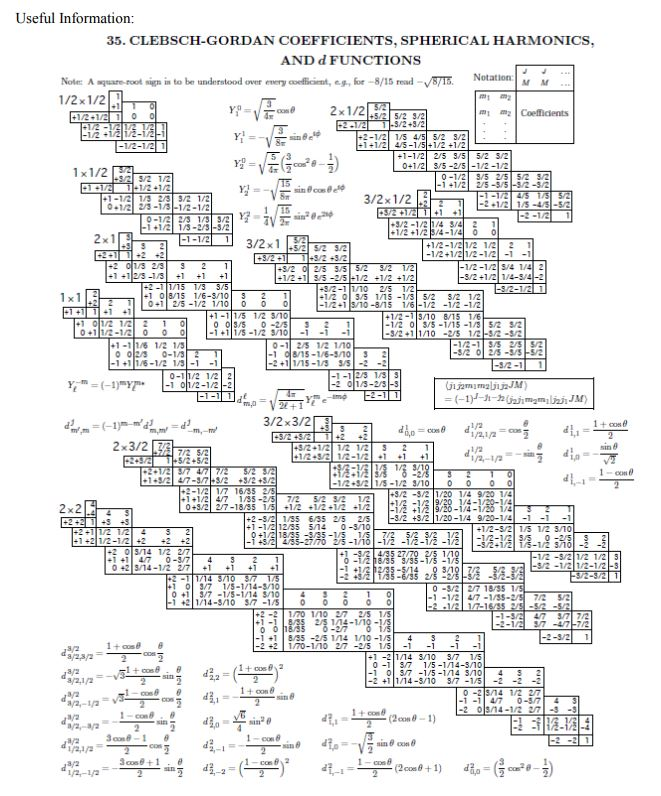
\includegraphics[width=\textwidth]
		{images/TCG.png}
		\caption{\label{fig:my-label} Tavole di C-G con annesse armoniche sferiche}}
\end{figure}


Ovviamente tutto questo discorso ci permette di ricavare informazioni per ogni momento angolare composto, che sia esso orbitale $L=l_1+l_2$, di spin $S=s_1+s_2$ o totale $J= L+S$


\newpage

\subsection{Stati di singoletto e tripletto}

Un caso molto interessante di composizione dei momenti riguarda quello degli spin degli elettroni.

Presi due elettroni con
\begin{align}
&s_1=\frac{1}{2}=s_2 \\
&s_z=\pm \frac{1}{2}
\end{align}

Nella base $\ket{s_{z_1},s_{z_2}}$ avremo quattro possibilità:
\begin{align}
\ket{+,+} \quad;\quad \ket{+,-} \quad;\quad \ket{-,+} \quad;\quad \ket{-,-}
\end{align}

Invece nella base $\ket{S_T,S_{T_z}}$ avremo che
\begin{align}
{}& s_1-s_2 \leq S_T \leq s_1+s_2 \rightarrow S_T=0,1 \; ;\; S_{T_z}=0,\pm 1 \\
& \ket{1,+1} \quad;\quad \ket{1,0} \quad;\quad \ket{1,-1} \quad;\quad \ket{0,0}
\end{align}

dove avremo gli stati simmetrici rispetto allo scambio di elettroni
\begin{align}
{}&\ket{1,+1} = \ket{+,+} \\
&\ket{1,-1} = \ket{-,-} \\
\end{align}

Come troviamo $\ket{1,0}$? Immaginiamo di applicare a $\ket{1,+1}$ l'operatore di discesa $S_-= S_x - iS_y$. 

Lo stato $\ket{1,+1= }\ket{+,+}$ è però \textbf{simmetrico allo scambio di elettroni} e anche l'operatore $S_-=s_{1_-}+s_{2_-}$ lo è, quindi anche $S_-\ket{+,+}$ lo sarà. Questo vuol dire che la combinazione di $\ket{+,-}$ e di $\ket{-,+}$ dovrà esserlo, e l'unica possible sarà
\begin{align}
&\ket{1,0} = \frac{1}{\sqrt{2}}(\ket{+,-} + \ket{-,+})
\end{align}

E abbiamo così trovato gli stati simmetrici detti di \textbf{tripletto}, mentre quello di \textbf{singoletto} sarà l'unica combinazione ortogonale rimasta, ovvero l'antisimmetrica:
\begin{align}
&\ket{0,0} = \frac{1}{\sqrt{2}}(\ket{+,-} - \ket{-,+})
\end{align}

\newpage

\section{L'operatore di scambio e il principio di Pauli}

Il discorso del P.d.P. nasce dal fatto che, presi due elettroni, se il problema si studia solo spazialmente essi sono indistinguibili.

Prendiamo un sistema composto dai suddetti:
\begin{align}
\ket{q,p,s}_1 \quad;\quad \ket{q,p,s}_2
\end{align}

Se queste sono davvero identiche deve essere per forza che \textbf{le funzioni associate devono essere simmetriche per scambio di particelle}, altrimenti avremmo un assurdo.

Introduciamo quindi l'\textbf{operatore di scambio} $\Pi$:
\begin{align}
\left\{
\begin{array}{cc}
\Pi q_1\Pi^{-1}=q_2 \\
\Pi q_2\Pi^{-1}=q_1
\end{array}
\right.
\quad ; \quad
\left\{
\begin{array}{cc}
\Pi p_1\Pi^{-1}=p_2 \\
\Pi p_2\Pi^{-1}=p_1
\end{array}
\right.
\quad ; \quad
\left\{
\begin{array}{cc}
\Pi s_1\Pi^{-1}=s_2 \\
\Pi s_2\Pi^{-1}=s_1
\end{array}
\right.
\end{align}

Si può anche dire che l'indistinguibilità delle particelle si traduce nel fatto che tutte le osservabili del sistema commutano con $\Pi$.

Per il \textbf{th. di Von Neumann} sappiamo che l'operatore associato a $\Pi$ è unico e unitario, e quindi
\begin{align}
\Pi\ket{A,B}=e^{i\phi}\ket{B,A}
\end{align}
poniamo
\begin{align}
{}&\Pi^2=1\\
&\Pi^{-1}=\Pi^\dagger=\Pi
\end{align}

Da cui segue che, chiamati gli stati \textbf{simmetrici} $\ket{S}$ e quelli \textbf{antisimmetrici} $\ket{A}$ gli unici autovalori possibili sono
\begin{align}
{}&\Pi\ket{S} = +1\ket{S} \\
&\Pi\ket{A} = -1\ket{A}
\end{align}

Una volta definiti questi due tipi di stati possiamo riscrivere tutti gli stati come combinazione di questi due tipi. In altre parole tutti gli stati vivono in uno spazio dato da
\begin{align}
H=H_S \otimes H_A
\end{align}

Qualora uno stato viva solo in uno dei due vi rimane per sempre.

\subsection{Principio di Pauli}

Se consideriamo l'atomo di elio e ci concentriamo sull'orbitale, sappiamo sperimentalmente che tale sistema è desritto dallo stato
\begin{align}
\ket{1s^2;S=0}
\end{align}
mentre è impossibile avere
\begin{align}
\ket{1s^2;S=1}
\end{align}

che in teoria sarebbe uno stato possibile. Questa evidenza sperimentale ci porta a due conseguenze:

\begin{enumerate}
	\item non tutti gli stati di $H$ rappresentano stati fisici 
	\item preso un sistema di due elettroni, l'unico stato possibile è quello antisimmetrico.
\end{enumerate}

Definite ora le famiglie di particelle

\begin{enumerate}
	\item \textbf{Fermioni}: particelle a spin semintero (elettroni, protoni, neutroni,...)
	\item \textbf{Bosoni}: particelle a spin intero (mesoni $\pi$,...)
\end{enumerate}

possiamo enunciare il \textbf{Principio di Pauli per il caso fermionico}:

\textit{Preso un sistema di due o più fermioni, gli unici stati possibili sono quelli rappresentati da vettori antisimmetrici rispetto allo scambio di una qualunque coppia di fermioni.}

Per il \textbf{caso bosonico} il discorso è analogo, ma gli stati sono invece \textbf{simmetrici}.

\newpage

Notiamo come per il princio di Pauli il numero di stati per un sistema a particelle identiche sia minore di quello per un sistema a particelle indistinguibili, infatti

\begin{enumerate}
	\item $e^+ \quad;\quad e^-$
	\begin{enumerate}
		\item $\ket{A}_+ \ket{B}_-$
		\item $\ket{B}_+ \ket{A}_-$
	\end{enumerate}
	
	\item $e^- \quad;\quad e^-$
	\begin{enumerate}
		\item $\ket{A}_-\ket{B}_- - \ket{B}_-\ket{A}_-$
	\end{enumerate}
\end{enumerate}

Il che si traduce anche nel dire che \textbf{un sistema a particelle identiche non è mai a variabili separabili e i suoi stati non sono mai fattorizzati}.

Il P.d.P. spiega anche perché gli orbitali possono ospitare al massimo due elettroni, in quanto \textbf{è impossibile creare uno stato di spin di tre o più elettroni antisimmetrico rispetto allo scambio dei numeri di spin di ogni coppia}:

\begin{enumerate}
	\item $\ket{+,+,+} \quad;\quad \ket{-,-,-}$
	
	Questi stati sono totalmente simmetrici
	
	\item $\ket{+,+,-} \quad;\quad \ket{+,-,+} \quad;\quad \ket{-,+,+}\quad;\quad \ket{-,-,+}\quad;\quad \ket{-,+,-}\quad;\quad \ket{+,-,-}$
	
	Questi stati sono simmetrici rispetto ad uno scambio e nessuna combinazione sarà mai completamente antisimmetrica
\end{enumerate}

Un'altra interessante questione deriva dal fatto che \textbf{tutte le informazioni relative alle proprietà di uno stato sono contenute nella collezione dei valori medi delle osservabili}

\begin{enumerate}
	\item \textbf{Particelle distinguibili:} $\ket{X}=\ket{A_1,B_2}$
	\begin{align}
	\braket{X|\xi|X}= \braket{A_1,B_2|\xi|A_1,B_2}
	\end{align}
	
	\item \textbf{Particelle indistinguibili:} $\ket{Y}=\frac{1}{\sqrt{2}}(\ket{A_1,B_2} \pm \ket{B_1,A_2})$	
		\begin{align}
		\braket{Y|\xi|Y} {}&= \frac{1}{2}(\bra{A_1,B_2} \pm \bra{B_1,A_2})\xi(\ket{A_1,B_2} \pm \ket{B_1,A_2}) = \nonumber \\
		&= \frac{1}{2}(\braket{A_1,B_2 |\xi| A_1,B_2} + \braket{B_1,A_2 |\xi| B_1,A_2}) + \nonumber \\
		&\quad + \frac{1}{2}(\pm \braket{A_1,B_2 |\xi| B_1,A_2} \pm \braket{B_1,A_2 |\xi| A_1,B_2})
		\end{align}
		ma dato che 
		\begin{align}
		\left\{
		\begin{array}{cc}
		\Pi=\Pi^{-1} \\
		\Pi\ket{A,B}=\ket{B,A}
		\end{array}		
		\right. 
		\end{align}
		avremo 
		\begin{align}	
		\braket{B_1,A_2|\xi|B_1,A_2}=\braket{B_1,A_2|\Pi^\dagger\xi\Pi|B_1,A_2}= \braket{A_1,B_2|\xi|A_1,B_2} \\
		\braket{B_1,A_2|\xi|A_1,B_2}= \braket{B_1,A_2|\Pi^\dagger\xi\Pi|A_1,B_2}= \braket{A_1,B_2|\xi|B_1,A_2}
		\end{align}
		da cui
		\begin{align}
		\braket{Y|\xi|Y} = \braket{A_1,B_2 |\xi| A_1,B_2} \pm \braket{A_1,B_2 |\xi| B_1,A_2}
		\end{align}
				
		Il secondo termine viene detto \textbf{di interferenza}, e il segno dipende dal tipo di particella (fermioni o bosoni).
\end{enumerate}

Notiamo che un sistema di particelle identiche con termine di interferenza nullo si tratta esattamente come un sistema di particelle indistinguibili. Questo spiega perché quando si studia un singolo atomo (per esempio H) non è necessario considerare gli altri elettroni nel sistema universo. 

Infatti se due sistemi descritti dagli stati $\ket{A}$ e $\ket{B}$ \textbf{sono lontani e localizzati} e quindi le loro funzioni d'onda $\psi_A(x)$ e $\psi_B(x)$ hanno \textbf{supporti disgiunti}, il termine di interferenza si annulla e si possono studiare i sottosistemi indipendentemente.

Il discorso è lo stesso anche  in caso di rappresentazione degli impulsi, in quanto
\begin{align}
p=-i \hbar \frac{\partial}{\partial x}
\end{align}

E i supporti delle derivate sono gli stessi delle funzioni di partenza. 
\chapter{Teoria delle perturbazioni}

La teoria delle perturbazioni è uno strumento molto potente nello studio di sistemi complessi. Il procedimento si basa sullo scomporre il sistema studiato in un caso noto (ex. l'Oscillatore Armonico) per poi aggiungere mano a mano piccoli contributi fino ad approssimare quanto si vuole il sistema da studiare.

\section{Perturbazioni indipendenti dal tempo}

Supponiamo di avere
\begin{align}
H^0\psi_n^0=E_n^0\psi_n^0 \quad ; \quad \braket{\psi_m^0|\psi_n^0}=\delta_{mn}
\end{align}
Immaginiamo ora di sommare un piccolo contributo. Avremo
\begin{align}
H\psi_n=E_n\psi_n 
\end{align}
con
\begin{align}
{}&H= H^0 + \lambda H'\\
&\lim_{\lambda \rightarrow 0}H= H^0
\end{align}

Espandiamo in serie le funzioni d'onda e gli autovalori dell'energia in funzione di $\lambda$:
\begin{align}
{}&\psi_n= \psi^0_n + \lambda \psi_n^1+ \lambda^2 \psi_n^2+\dots \\
&E_n= E_n^0 + \lambda E_n^1+ \lambda^2 E_n^2+\dots
\end{align}

Questo ci porta a riscrivere, 
\begin{align}
{}&H^0\psi^0_n=E^0_0n\psi^0_n	\qquad \text{eq. imperturbata}\\
&\lambda(H^0\psi'_n + H'\psi^0_n)=\lambda(E'_n \psi^0_n + E^0_n\psi'_n) \qquad\qquad\qquad\qquad\qquad\,\, \text{I ordine}\\
&\lambda^2 (H^0\psi^2_n + H'\psi'_n)=\lambda^2 (E^0_n \psi^2_n + E^0_n \psi_n^2 + E_n^2\psi_n^0 + E_n'\psi_n')\qquad \text{II ordine} \\
\vdots \nonumber
\end{align}

\subsection{Perturbazione al I ordine}

\begin{align}
H^0\psi_n' + H'\psi_n^0= E_n'\psi_n^0 + E_n^0\psi_n' 
\end{align}

Moltiplicando entrambi i lati per il complesso coniugato di $\psi_n^0$ possiamo scrivere, passando in notazione di Dirac:
\begin{align}
\braket{\psi_n^0 |H^0|\psi_n'} + \braket{\psi_n^0 |H'|\psi_n^0} = E_n'\braket{\psi_n^0|\psi_n^0} + E_n^0 \braket{\psi_n^0|\psi_n'}
\end{align}

Siccome non sappiamo nulla delle $\psi_n'$ possiamo supporre che essa sia ortogonale a $\psi_n^0$, e quindi, ricordando che H è hermitiano:
\begin{align}
E_n^0 \, \cancel{\braket{\psi_n^0 |\psi_n'}}+ \braket{\psi_n^0 |H'|\psi_n^0}= E_n' + E_n^0 \, \cancel{\braket{\psi_n^0 |\psi_n'}}
\end{align}
ossia
\begin{align}
E_n'=\braket{\psi_n^0 |H'|\psi_n^0}
\end{align}

ed abbiamo così trovato la correzione dell'energia  al primo ordine.

Che forma avranno invece le correzioni alle autofunzioni?

Ricordiamo che se le $\psi_n^0$ formano un set di autofunzioni completo possiamo riscrivere le $\psi_n'$ come combinazioni lineari di queste:
\begin{align}
\psi_n'= \sum_{m\neq n}c_m^{(n)}\psi_m^0
\end{align}

La condizione $m\neq n$ è necessaria in quanto se $\psi_n'$ è soluzione dell'equazione sicuramente lo sarà la combinazione $\psi_n' + \alpha \psi_n^0$ con $\alpha=cost.$

\newpage

Questo ci porta ad avere l'eq.di Schrödinger nella forma
\begin{align}
(H^0 - E^0_n)\ket{\psi_n'} = (H^0 - E^0_n)\sum_{m\neq n}c_m^{(n)}\ket{\psi_m^0} = -(H'-E')\ket{\psi_n^0}
\end{align}
che possiamo riscrivere
\begin{align}
\sum_{m\neq n}c_m^{(n)} (E_m^0 - E^0_n) \ket{\psi_m^0} = -(H'-E')\ket{\psi_n^0}
\end{align}
Se ora moltiplichiamo per una generica $\ket{\psi_k^0}$ otteniamo
\begin{align}
\sum_{m\neq n}c_m^{(n)} (E_m^0 - E^0_n) \braket{\psi_k^0|\psi_m^0} = -(H'-E')\braket{\psi_k^0|\psi_n^0}
\end{align}
Notiamo che se $k=n$ il termine a sinistra si annulla, quindi deve essere $k\neq n$, da cui
\begin{align}
\sum_{m\neq n}c_m^{(n)} (E_m^0 - E^0_n)\delta_{km} = -\braket{\psi_k^0|H'|\psi_n^0} +E'\, \cancel{\braket{\psi_k^0|\psi_n^0}}
\end{align}
che diventa
\begin{align}
{}&c_m^{(n)} (E_m^0 - E^0_n) = -\braket{\psi_k^0|H'|\psi_n^0}\\
&\downarrow \nonumber \\
\label{eq:eq0}
& c_m^{(n)}  = \frac{\braket{\psi_k^0|H'|\psi_n^0}}{E_n^0 - E^0_m}
\end{align}
da cui otteniamo infine
\begin{align}
\psi_n'= \sum_{m\neq n} \frac{\braket{\psi_k^0|H'|\psi_n^0}}{E_n^0 - E^0_m} \psi_m^0
\end{align}

\subsection{Perturbazione al II ordine}

Ricordiamo che al II ordine abbiamo:
\begin{align}
         \label{eq:eq1}
H^0\psi^2_n + H'\psi'_n=E^0_n \psi^2_n + E^2_n \psi_n^0 + E_n^2\psi_n^0 + E_n'\psi_n'
\end{align}

Avremo di nuovo:
\begin{align}
\label{eq:eq2}
\psi_n'= \sum_{m\neq n}c_m^{(n)}\psi_m^0
\end{align}

ma stavolta dobbiamo tenere da conto anche $\psi_n^2$, di cui non sappiamo nulla.

Partiamo di nuovo dalle correzioni sull'energia. Passiamo in notazione di Dirac per comodità e moltiplichiamo da entrambi i lati per $\bra{\psi_n^0}$ la $\eqref{eq:eq1}$. Ricordando le considerazioni del paragrafo scorso otteniamo 
\begin{align}
\label{eq:eq3}
{}& \braket{\psi_n^0|H^0|\psi^2_n} + \braket{\psi_n^0|H'|\psi'_n}=E^0_n\cancel{\braket{\psi_n^0|\psi^2_n}} + E^2_n\braket{\psi_n^0|\psi_n^0} + E_n'\cancel{\braket{\psi_n^0|\psi_n'}}\nonumber \\
& \downarrow \\
& E_n^0\cancel{\braket{\psi_n^0|\psi^2_n}} + \braket{\psi_n^0|H'|\psi'_n}= E^2_n\braket{\psi_n^0|\psi_n^0}\nonumber \\
& \downarrow \\
& E^2_n=\braket{\psi_n^0|H'|\psi'_n}
\end{align}

Vista la $\eqref{eq:eq2}$ e la $\eqref{eq:eq0}$ possiamo scrivere
\begin{align}
E^2_n{}&=\sum_{m\neq n} c_m\braket{\psi_n^0|H'|\psi^0_m} \\
&= \sum_{m\neq n}\frac{\braket{\psi_m^0|H'|\psi_n^0} \braket{\psi_n^0|H'|\psi^0_m}}{E_n^0 - E^0_m}
\end{align}

Notiamo come il denominatore non crei problemi fintantoché lo spettro energetico degli stati imperturbati è non degenere.

Siccome $|x^2|= x^* x$ e $\braket{\psi_m^0|H'|\psi_n^0}= (\braket{\psi_n^0|H'|\psi^0_m})^*$ possiamo scrivere in modo più compatto
\begin{align}
E^2_n= \sum_{m\neq n}\frac{|\braket{\psi_m^0|H'|\psi_n^0}|^2}{E_n^0 - E^0_m}
\end{align}

\newpage

\subsection{Caso degenere}

Affrontiamo ora il problema della degenerazione.
Avremo, dato un livello dell'energia imperturbata
\begin{align}
E_d^0 \; t.c. \left\{\begin{array}{cc}
H^0\ket{\psi^0_a}= E_d^0\ket{\psi^0_a} \\
H^0\ket{\psi^0_b}= E_d^0\ket{\psi^0_b}
\end{array}
\right. \quad ; \quad \braket{\psi_a^0 | \psi_b^0}=0
\end{align}

Sappiamo già che anche $\ket{\psi^0}= \alpha \ket{\psi^0_a} + \beta \ket{\psi^0_b}$ sarà autofunzione di $H$ tale che $H^0\ket{\psi^0}=E_d^0\ket{\psi^0}$.

Cosa accade quando si perturba l'energia?

Nel migliore dei casi si ha una rimozione della degenerazione, e che quando "spegniamo" la perturbazione $H'$ (cioè si ha $\lambda \rightarrow 0$)avremo che
\begin{enumerate}
	\item lo stato ad energia più alta cadrà in una combinazione $\ket{\psi_1}$ tra $\ket{\psi^0_a}$ e $\ket{\psi^0_b}$
	\item lo stato ad energia più bassa cadrà in una combinazione
	$\ket{\psi_2}\neq \ket{\psi_1}$
\end{enumerate} 

Iniziamo dal punto di partenza del caso non degenere. Al I ordine avremo
\begin{align}
H^0\ket{\psi'} + H'\ket{\psi^0}=E^0\ket{\psi'} + E'\ket{\psi^0}
\end{align}

moltiplichiamo tutto per $\bra{\psi_a^0}$ e otteniamo
\begin{align}
{}&\braket{\psi_a^0|H^0|\psi^1} + \braket{\psi_a^0|H'|\psi^0} = E^0 \cancel{\braket{\psi_a^0|\psi'}} + E'\braket{\psi_a^0|\psi^0}\\
&\downarrow \nonumber \\
&E^0\cancel{\braket{\psi_a^0|\psi^1}} + \braket{\psi_a^0|H'|\psi^0} =  E'\braket{\psi_a^0|\psi^0}\\
&\downarrow \nonumber \\
&\braket{\psi_a^0|H'|\psi^0} =  E'\braket{\psi_a^0|\psi^0}\\
&\downarrow \nonumber \\
&\bra{\psi_a^0}H'(\alpha \ket{\psi^0_a} + \beta \ket{\psi^0_b})= E'\bra{\psi_a^0}(\alpha \ket{\psi^0_a} + \beta \ket{\psi^0_b}) \\
&\downarrow \nonumber \\
&\alpha \braket{\psi_a^0 |H'|\psi_a^0} + \beta\braket{\psi_a^0 |H'|\psi_b^0} = E' ( \alpha \braket{\psi_a^0|\psi_a^0} + \beta \cancel{\braket{\psi_a^0|\psi_b^0}} )
\end{align}
chiamiamo
\begin{align}
W_{aa}= \braket{\psi_a^0 |H'|\psi_a^0} \\
W_{ab}= \braket{\psi_a^0 |H'|\psi_b^0}
\end{align}
e riscriviamo così
\begin{align}
\alpha E' = \alpha W_{aa} + \beta W_{ab}
\end{align}
svolgendo gli stessi conti con $\bra{\psi_b^0}$
\begin{align}
{}&W_{ba}= \braket{\psi_b^0 |H'|\psi_a^0} \\
&W_{bb}= \braket{\psi_b^0 |H'|\psi_b^0}\\
&\beta E' = \alpha W_{ba} + \beta W_{bb}
\end{align}
moltiplichiamo $E'$ nella seconda per $W_{ab}$ ottenendo
\begin{align}
{}&\beta E' W_{a_b} = \alpha W_{ba}W_{a_b} + \beta W_{bb}W_{a_b} \\
&\downarrow \nonumber \\
&E' \beta  W_{a_b} = \alpha W_{ba}W_{a_b} + \beta W_{bb}W_{a_b}
\end{align}
e sostituiamo, ricavandolo dall'altra, $\beta W_{ab}= \alpha E' - \alpha W_{aa}$ ottenendo
\begin{align}
{}&E' \alpha E' - E'\alpha W_{aa} = \alpha W_{a_b}W_{ba} + \beta W_{a_b}W_{bb} \\
&\downarrow \nonumber \\
&\alpha W_{a_b}W_{ba} + W_{bb}[\alpha E' - \alpha W_{aa}] - E'[\alpha E' - \alpha W_{aa}]=0 \\
&\downarrow \nonumber \\
& \alpha [W_{a_b}W_{ba} - (E'-W_{bb})(E' - W_{aa})] =0
\end{align}

\newpage

\textbf{Qualora $\alpha \neq 0$}:
\begin{align}
(E')^2 - E'(W_{aa} + W_{bb}) - (W_{aa}W_{bb} - W_{ab}W_{ba})=0
\end{align}
Abbiamo così un'equazione lineare al II ordine, le cui soluzioni saranno
\begin{align}
E'_\pm = \frac{1}{2} [W_{aa} + W_{bb} \pm \sqrt{(W_{aa}-W_{bb})^2 + 4|W_{ab}|^2}]
\end{align}
Abbiamo così trovato le correzioni all'energia.

Cosa succede se uno dei due coefficienti è nullo? Semplicemente ci si riconduce al caso non degenere.

\section{Perturbazioni dipendenti dal tempo (incomplete)}

Studiamo il problema nel caso di un \textbf{sistema a due livelli}. Avremo solo due livelli energetici possibili per l'hamiltoniana imperturbata:
\begin{align}
{}&\left\{\begin{array}{cc}
H^0\ket{\psi^0_a}= E_a^0\ket{\psi^0_a} \\
H^0\ket{\psi^0_b}= E_b^0\ket{\psi^0_b}
\end{array}
\right. \quad;\quad \braket{\psi_a^0 |\psi_b^0}= \delta_{ab} \\
\nonumber \\
&\ket{\psi^0}= c_a\ket{\psi^0_a} + c_b\ket{\psi^0_b}
\end{align}
In assenza di perturbazioni, in caso di evoluzione temporale essi evolvono indipendentemente:
\begin{align}
{}&\ket{\psi^0}= c_a e^{-i \frac{E_a}{\hbar}t} \ket{\psi^0_a} + c_b e^{-i \frac{E_b}{\hbar}t} \ket{\psi^0_b} \\
&|\psi^0|^2= |c_a|^2 + |c_b|^2=1
\end{align}
Aggiungiamo una perturbazione $H'(t)$ dipendente dal tempo. Le autofunzioni dovranno rimanere uguali, correzioni permettendo, ma avremo dei coefficienti dipendenti dal tempo, dato che se scriviamo $\psi(r,t) = \psi(r)e^{-i \frac{E}{\hbar}t}$ nell'equazione di Schroedinger $V(r,t)$ agirà solo su $\psi(r)$, e il risultato di tale applicazione saranno proprio i coefficienti.

Cerchiamo quindi una soluzione del tipo
\begin{align}
\ket{\psi^0}= c_a(t) e^{-i \frac{E_a}{\hbar}t} \ket{\psi^0_a} + c_b(t) e^{-i \frac{E_b}{\hbar}t} \ket{\psi^0_b}
\end{align}
Ricordando che
\begin{align}
&H= H^0 + H'(t) \\
&H\psi = i \hbar \frac{\partial}{\partial t} \psi
\end{align}
Possiamo riscrivere
\begin{align}
&(H^0 + H'(t))(c_a(t) e^{-i \frac{E_a}{\hbar}t} \psi^0_a + c_b(t) e^{-i \frac{E_b}{\hbar}t} \psi^0_b)=  i \hbar \frac{\partial}{\partial t} \psi^0\\
\downarrow \nonumber \\
& c_a(t) e^{-i \frac{E_a}{\hbar}t} H^0\psi^0_a + c_a(t) e^{-i \frac{E_a}{\hbar}t}H'(t)\psi^0_a +  c_b(t) e^{-i \frac{E_b}{\hbar}t} H^0\psi^0_b + c_b(t) e^{-i \frac{E_b}{\hbar}t}H'(t)\psi^0_b=  \nonumber \\
&=i\hbar \left[ \dot{c_a}\psi^0_a e^{-i \frac{E_a}{\hbar}t} -i\frac{E_a}{\hbar}c_a\psi^0_a e^{-i \frac{E_a}{\hbar}t} + 
\dot{c_b}\psi^0_b e^{-i \frac{E_b}{\hbar}t} -i\frac{E_b}{\hbar}c_a\psi^0_b e^{-i \frac{E_b}{\hbar}t}
\right]\\
&c_a(t) e^{-i \frac{E_a}{\hbar}t} E_a^0\psi^0_a + c_a(t) e^{-i \frac{E_a}{\hbar}t}H'(t)\psi^0_a +  c_b(t) e^{-i \frac{E_b}{\hbar}t} E_b^0\psi^0_b + c_b(t) e^{-i \frac{E_b}{\hbar}t}H'(t)\psi^0_b=  \nonumber \\
&= i\hbar \left[
\dot{c_a}\psi^0_a e^{-i \frac{E_a}{\hbar}t} + \dot{c_b}\psi^0_b e^{-i \frac{E_b}{\hbar}t}
\right]
+ c_a(t) e^{-i \frac{E_a}{\hbar}t} E_a^0\psi^0_a +  c_b(t) e^{-i \frac{E_b}{\hbar}t} E_b^0\psi^0_b \nonumber \\
&\downarrow \nonumber \\
&c_a(t) e^{-i \frac{E_a}{\hbar}t}H'(t)\psi^0_a + c_b(t) e^{-i \frac{E_b}{\hbar}t}H'(t)\psi^0_b= i\hbar \left[
\dot{c_a}\psi^0_a e^{-i \frac{E_a}{\hbar}t} + \dot{c_b}\psi^0_b e^{-i \frac{E_b}{\hbar}t}
\right]
\end{align}

Proviamo ora ad isolare i due coefficienti.

Iniziamo passando in notazione di Dirac e prima moltiplicando per $\bra{\psi_a^0}$:
\begin{align}
c_a e^{-i \frac{E_a}{\hbar}t} \braket{\psi_a^0|H'|\psi_a^0} + 
c_b e^{-i \frac{E_b}{\hbar}t} \braket{\psi_a^0|H'|\psi_b^0} = i \hbar \dot{c_a} e^{-i \frac{E_a}{\hbar}t}
\end{align}

definiamo ora per pulizia $H'_{ij} = \braket{\psi_i|H'|\psi_j}$ e $\omega_{ij}=E_i - E_j$. 

Ci rendiamo conto di essere di fronte ad un'equazione differenziale:
\begin{align}
\dot{c_a} = -\frac{i}{\hbar}[H'_{aa} c_a + H'_{ab} e^{i\frac{\omega_{ab}}{\hbar}t} c_b]
\end{align}
In modo più compatto per casi più generali:
\begin{align}
\dot{c_m}(t)= -\frac{i}{\hbar}\sum_n H'_{mn} e^{i\frac{\omega_{mn}}{\hbar}t}c_n
\end{align}

ROBA DA CHIEDERE POCO CHIARA, APPUNTI PERSI

\subsection{Oscillazioni armoniche (mancanti)}

Supponiamo di avere una dipendenza temporale della forma

\begin{align}
H'(r,t)= V(r) \cos{\omega t} \rightarrow H'_{ab}= \braket{\psi_a|V|\psi_b} \cos{\omega t} = V_{ab}\cos{\omega t}
\end{align}

Supponiamo che gli elementi diagonali siano nulli.

*APPUNTI PERSI*

\backmatter
% bibliography, glossary and index would go here.

\end{document}